\def\printmanual{true}
% arara: makeindex

% Template for IEEE papers
%% bare_conf.tex
%% V1.4b
%% 2015/08/26
%% by Michael Shell
%% See:
%% http://www.michaelshell.org/
%% for current contact information.
%%
%% This is a skeleton file demonstrating the use of IEEEtran.cls
%% (requires IEEEtran.cls version 1.8b or later) with an IEEE
%% conference paper.
%%
%% Support sites:
%% http://www.michaelshell.org/tex/ieeetran/
%% http://www.ctan.org/pkg/ieeetran
%% and
%% http://www.ieee.org/

%%*************************************************************************
%% Legal Notice:
%% This code is offered as-is without any warranty either expressed or
%% implied; without even the implied warranty of MERCHANTABILITY or
%% FITNESS FOR A PARTICULAR PURPOSE!
%% User assumes all risk.
%% In no event shall the IEEE or any contributor to this code be liable for
%% any damages or losses, including, but not limited to, incidental,
%% consequential, or any other damages, resulting from the use or misuse
%% of any information contained here.
%%
%% All comments are the opinions of their respective authors and are not
%% necessarily endorsed by the IEEE.
%%
%% This work is distributed under the LaTeX Project Public License (LPPL)
%% ( http://www.latex-project.org/ ) version 1.3, and may be freely used,
%% distributed and modified. A copy of the LPPL, version 1.3, is included
%% in the base LaTeX documentation of all distributions of LaTeX released
%% 2003/12/01 or later.
%% Retain all contribution notices and credits.
%% ** Modified files should be clearly indicated as such, including  **
%% ** renaming them and changing author support contact information. **
%%*************************************************************************


% *** Authors should verify (and, if needed, correct) their LaTeX system  ***
% *** with the testflow diagnostic prior to trusting their LaTeX platform ***
% *** with production work. The IEEE's font choices and paper sizes can   ***
% *** trigger bugs that do not appear when using other class files.       ***                          ***
% The testflow support page is at:
% http://www.michaelshell.org/tex/testflow/

\documentclass{book}
\usepackage[quiet]{fontspec}
\usepackage[table,xcdraw,dvipsnames]{xcolor} % Used by spritegrid and others.
\usepackage[obeyspaces,spaces]{url}
\usepackage{longtable}
\usepackage{arydshln}
\usepackage{booktabs}
\usepackage{afterpage}
\usepackage{flushend}
\usepackage{titletoc}
\usepackage[toc]{appendix}
\usepackage{parskip}
\usepackage{graphicx,wrapfig}
\usepackage{float}
\usepackage{caption}
\usepackage{pdfpages}
\usepackage{tikzpagenodes}
\usepackage{imakeidx}
\usepackage[pagestyles,raggedright]{titlesec}
\usepackage[all]{nowidow}
\usepackage[bookmarks=true]{hyperref}
\usepackage{aeb-minitoc}
\usepackage{fix-cm}
\usepackage{textpos}
\usepackage{enumitem}
\usepackage{tcolorbox}
\tcbuselibrary{breakable,listings,skins,xparse}
%\usepackage{wrapfig}
\usepackage{needspace}
\usepackage{verbatim}
\usepackage{ean13isbn}
\usepackage{setspace}

% Use CHAPTER-PAGE page numbering to make it easier to modify chapters
% later, without messing up page number of the rest of the book.
\usepackage[auto]{chappg}

% Allow cross-references between the various books to the big The MEGA65 Book
\usepackage{xr}
\usepackage{varioref}
\usepackage{xparse}
\externaldocument[M65Book-]{mega65-book}
% And a \ref alternative that checks if it needs to be a cross-reference to the
% MEGA65 Book instead.
\makeatletter
\newcommand{\bookref}[1]{%
    \@ifundefined{r@#1}{%
      {\em the MEGA65 Book}, \nameref{M65Book-#1} (\autoref{M65Book-#1})}{\autoref{#1}}%
}
\newcommand{\bookvref}[1]{%
    \@ifundefined{r@#1}{%
      {\em the MEGA65 Book}, \nameref{M65Book-#1} (\autoref{M65Book-#1})}{Chapter/Appendix \vref{#1}}%
}
\makeatother

% For fixed-width columns in register maps
\usepackage{array}

% Makes tables with double-ruled lines look better
\usepackage{hhline}

% Makes better use of space for reference tables in appendix
\usepackage{multicol}

% Shaded tables with alternate rows colored for better legibility
% Best used with larger tables rather than small tables
\usepackage{colortbl}
\usepackage{adjustbox}
\usepackage[strict]{changepage}

% \makecell command for forcing line breaks in table cells
\usepackage{makecell}

\newcolumntype{L}[1]{>{\raggedright\let\newline\\\arraybackslash\hspace{0pt}}m{#1}}
\newcolumntype{C}[1]{>{\centering\let\newline\\\arraybackslash\hspace{0pt}}m{#1}}
\newcolumntype{R}[1]{>{\raggedleft\let\newline\\\arraybackslash\hspace{0pt}}m{#1}}

% For displaying Letter keys and the MEGA key
% This is a `keys' element for displaying a Mega65 keyboard key
% using a black filled label with rounded edges.
% In order to display a key as a title, use:
%
%     \megakey[title]{Run/Stop}
%
% For displaying a key as a part of the normal document flow, simply use:
%
%    \specialkey{SHIFT}
%
%
% If you get warnings on special characters, mathematical characters etc, use $, eg:
%
%    \megakey{$\leftarrow$}
%
% Other sizes are supported, as part of tcolorbox:
% http://mirror.aarnet.edu.au/pub/CTAN/macros/latex/contrib/tcolorbox/tcolorbox.pdf#subsubsection.4.7.5 however, only `title' and the default: `small' are proposed for use in this manual.
%
% The second macro available here is the megasymbolkey.
% This will display the MEGA symbol as white on a black key box. Simply use:
%
%		 \megasymbolkey
%
% Some MEGA65 keys contain two lines of text like "RUN/STOP"
% You can use the specialkey macro for this:
%
%    \specialkey{SHIFT LOCK}%

\usepackage{tcolorbox}

\newtcbox{\megakeyinner}[1][small]{colback=black, coltext=white, size=#1, fontupper=\bfseries, nobeforeafter,box align=bottom,baseline=3pt,text height=7pt}
\newcommand{\megakey}[2][small]{\megakeyinner[#1]{\uppercase{#2}}}

% Previous version of megasymbolkey
%\newtcbox{\megasymbolkeyinner}{colback=black, coltext=white, clip title=false. fontupper=\symbolfont, box align=bottom,baseline=3pt,text height=7pt}
%\newcommand{\megasymbolkey}{\megakeyinner{\megasymbol[white]}\ }

\newtcolorbox{megasymbolkeyinner}
{colback=black,coltext=white,size=small,fontupper=\small\bfseries,
width=0.65cm, height=0.55cm, box align=base,
nobeforeafter, halign=flush left, left=0mm,top=0.3mm,bottom=0mm,right=0mm
,boxsep=0.5mm,baseline=4pt, enlarge right by = 1mm
}
\newcommand{\megasymbolkey}{
\begin{megasymbolkeyinner}%
\megasymbol[white]%
\end{megasymbolkeyinner}%
}

\newtcolorbox{specialkeyinner}
{colback=black,coltext=white,size=small,fontupper=\tiny\bfseries,
width=0.80cm, height=0.55cm, box align=base,
nobeforeafter, halign=flush left, left=0mm,top=0.3mm,bottom=0mm,right=0mm
,boxsep=0.5mm,baseline=4pt
}
\newcommand{\specialkey}[1]{
\begin{specialkeyinner}%
#1%
\end{specialkeyinner}%
}

\newtcolorbox{widekeyinner}
{colback=black,coltext=white,size=small,fontupper=\tiny\bfseries,
width=0.9cm, height=0.55cm, box align=base,
nobeforeafter, halign=flush left, left=0mm,top=0.3mm,bottom=0mm,right=0mm
,boxsep=0.5mm,baseline=4pt
}
\newcommand{\widekey}[1]{
\begin{widekeyinner}%
#1%
\end{widekeyinner}%
}




% For displaying print versions petscii character symbols
% This is a collection of symbol macros element for displaying a printed version of the
% MEGA65 graphic characters, as opposed to the bitmap versions in the mega40/80.ttf fonts files.
% You can display characters using the graphicsymbol macro:
%
%    \graphicsymbol{\textcolor{red}{qQ} wWUcbdhjI \textcolor{blue}{JK}}
%
% Or you can, simply use the font itself:
%
%    \begin{symbolfont}%
%	   qQwWeErRtTyYuUiIoOpP\\
%		 aAsSdDfFgGhHjJkKlL\\
%		 zZxXcCvVbBnNmM%
%		 \end{symbolfont}%
%
%
% You can display the MEGA symbol using:
%
%    \megasymbol
%
% This will display the symbol in black. Other colours can be specified by passing them in, for example:
%
% 	 \megasymbol[black]
%		 \megasymbol[white]
%		 \megasymbol[orange]
%		 \megasymbol[blue]
%
% NOTE:
% For using the MEGA symbol in a key, see the \megasymbolkey macro in the keys.txt file.

\usepackage{tcolorbox}

\newcommand{\graphicsymbol}[1]{\begin{symbolfont}#1\end{symbolfont}}

\newcommand{\megasymbol}[1][black]{\begin{symbolfont}\textcolor{#1}{`}\end{symbolfont}}


% For Mega65 display of code, listings and screen activity
\input{elements/screenoutput}

% For MEGA65 screen shots with text flow
\input{elements/screenshots}

% For displaying sprite data in a grid
% This is an element for displaying a sprite in a grid, just like page 70 of the
% commodore manual. This version can be easily expanded. For now it will suffice.
% In order to display a hi-res mono sprite grid use:
%
%	\spritegrid{
%	\hline
%	\spritecells{---------ooooo----------}
%	\spritecells{-------ooooooooo--------}
%	\spritecells{------ooooooooooo-------}
%	\spritecells{------ooo--o---oo-------}
%	\spritecells{-----ooo-ooo-ooooo------}
%	\spritecells{-----ooo-ooo-ooooo------}
%	\spritecells{-----ooo---o---ooo------}
%	\spritecells{-----ooo-o-ooo-ooo------}
%	\spritecells{-----ooo-o-ooo-ooo------}
%	\spritecells{-----ooo---o--oooo------}
%	\spritecells{------ooooooooooo-------}
%	\spritecells{------ooooooooooo-------}
%	\spritecells{-------ooooooooo--------}
%	\spritecells{-------o-ooooo-o--------}
%	\spritecells{--------o-o-o-o---------}
%	\spritecells{--------o--o--o---------}
%	\spritecells{---------o-o-o----------}
%	\spritecells{---------o-o-o----------}
%	\spritecells{---------ooooo----------}
%	\spritecells{---------ooooo----------}
%	\spritecells{----------ooo-----------}
%	}
%
% For a multicolour sprite:
%
%	\spritegrid{
%	\hline
%	\spritecells{------------------------}
%	\spritecells{------------------------}
%	\spritecells{------------------------}
%	\spritecells{------------------------}
%	\spritecells{llllllllllllllllllllllll}
%	\spritecells{llllllllllllllllllllllll}
%	\spritecells{lllllleeeeeelleeeeeeeell}
%	\spritecells{lllloooooooollooooooooll}
%	\spritecells{llllooggggggllooggggggll}
%	\spritecells{lllloolllllllloollllllll}
%	\spritecells{llllooeeeellllooeeeellll}
%	\spritecells{lllloooooooollooooooooll}
%	\spritecells{llllooggggoollggggggooll}
%	\spritecells{lllloolllloollllllllooll}
%	\spritecells{llllooeeeeoolleeeeeeooll}
%	\spritecells{llllggooooggllooooooggll}
%	\spritecells{llllllggggllllggggggllll}
%	\spritecells{llllllllllllllllllllllll}
%	\spritecells{------------------------}
%	\spritecells{------------------------}
%	\spritecells{------------------------}
%	}

\usepackage{tabulary} %Removes spacing from tabulars
\usepackage{xstring} % for string substitution
\usepackage{xparse} % used for unpacking the sprite characters
% \renewcommand{\familydefault}{\sfdefault} % default sans font

%\usepackage{graphicx} % for resizing the tabular used by spritegrid
\usepackage{subcaption} % used for the left hand subtable of row numbers
\usepackage{multirow} % used for the ``Row'' column
\usepackage{rotating} % used by the rotating ``Row'' word

\newcommand{\spritebytecolumn}[1]{
   %\framebox[4mm]{#1}
   \makebox[4mm]{#1}
}

\setlength\tabcolsep{0.3mm} % the indivdual cell width and height


% Cell colour list. Can be expanded for other colours in the sprite grid
\def\blk{\cellcolor{black}}
\def\wht{\cellcolor{white}}
\def\grn{\cellcolor{ForestGreen}}
\def\lgrn{\cellcolor{YellowGreen}}
\def\gry{\cellcolor{Gray}}

\newcounter{lettercounter} % counter for detecting the last cell

% Collect the spritecell list and send it to \ProcessSpriteCell for turning into cells
\NewDocumentCommand{\spritecells}{%
>{\SplitList{}} m }{%
  \ProcessList{#1}{\ProcessSpriteCell}%
}

\NewDocumentCommand{\ProcessSpriteCell}{m}{%
  \stepcounter{lettercounter}%
    \IfStrEqCase{#1}{
	{o}{\blk}
	{-}{\wht}
	{g}{\grn}
	{l}{\lgrn}
	{e}{\gry}
   }%
   \IfStrEq{\thelettercounter}{24}{\setcounter{lettercounter}{0} \\ \hline}{&}%
}

% Start of the actual spritegrid definition
\newcommand{\spritegrid}[1]{
\begin{table}[h!]
\centering
\begin{subtable}{28mm}
\vspace{8mm}
\scalebox{0.76}{
\begin{center}
\begin{tabular}{p{25mm} p{4mm} c}
\multirow{21}{*}{ } &
\multirow{21}{*}{%
\begin{turn}{90}%
\bfseries\uppercase{Row}%
\end{turn}} &
 1\\
& & 2\\
& & 3\\
& & 4\\
& & 5\\
& & 6\\
& & 7\\
& & 8\\
& & 9\\
& & 10\\
& & 11\\
& & 12\\
& & 13\\
& & 14\\
& & 15\\
& & 16\\
& & 17\\
& & 18\\
& & 19\\
& & 20\\
& & 21
\end{tabular}
\end{center}
}
\end{subtable}%
\begin{subtable}{.8\textwidth}

\setlength{\arrayrulewidth}{1pt}
\scalebox{0.7}{
\begin{center}
\begin{tabular}{  *{3}{p{30mm} }  }
  \center\uppercase{Series\\1} &
  \center\uppercase{Series\\2} &
  \center\uppercase{Series\\3}
\end{tabular}
\end{center}
}

\scalebox{0.7}{
\begin{center}
\begin{tabular}{p{5.8mm} *{11}{C{7.3mm}}}
   128 & 32 & 8 & 2 & 128 & 32 & 8 & 2 & 128 & 32 & 8 & 2
\end{tabular}
\end{center}
}
\\[-1.5mm]
\scalebox{0.7}{
\begin{center}
\begin{tabular}{p{1.7mm} *{12}{C{7.3mm}}}
  & 64 & 16 & 4 & 1 & 64 & 16 & 4 & 1 & 64 & 16 & 4 & 1
\end{tabular}
\end{center}
}

\scalebox{0.7}{
\begin{center}
\begin{tabular}{ | *{24}{p{3mm} |}  }
#1
\end{tabular}
\end{center}
}

\scalebox{0.7}{
\begin{center}
\begin{tabular}{ *{24}{p{3.35mm}}  }
	\spritebytecolumn{1} & & & &
	\spritebytecolumn{5} & & & & &
	\spritebytecolumn{10} & & & & &
	\spritebytecolumn{15} & & & & &
	\spritebytecolumn{20} & & & &
	\spritebytecolumn{24} \\
	\multicolumn{24}{c}{\bfseries\uppercase{Column}}
\end{tabular}
\end{center}
}
\end{subtable}
\end{table}
}

% End of the actual spritegrid definition



% Don't number sections
\setcounter{secnumdepth}{0}

\renewcommand{\indexname}{INDEX}
\renewcommand{\appendixtocname}{APPENDICES}
\renewcommand{\appendixpagename}{APPENDICES}
\renewcommand{\appendixpage}{%
  \clearpage\thispagestyle{empty}
    \pagecolor{blue}
     \begin{center}
       {
         \large
         % Put a nice amount of vertical space before the title
         \vspace*{2cm}
               {\large\Huge\textcolor{white}{\bf{APPENDICES}}}\\
             \vspace{\fill}
       }
     \end{center}
     \newpage\pagecolor{white}\clearpage
}

\makeatletter\chardef\pdf@shellescape=\@ne\makeatother

\setcounter{tocdepth}{5}

% 1.0 cm is the distance from left of page to bullet point.
% 2.8 cm is a fudge-factor to make multi-line section names be correctly lined up.
% \@B{〈length〉} is the amount to indent prior to〈sec-num >
% \@F{〈fmt〉} is the formatting for the title heading
% \@P{〈fmt〉} is the formatting for the page number (〈pg-num〉).

\TOCLevels{chapter}{section}
\begin{minitocfmt}{\chapmtoc}
\declaretocfmt{section}{\@F{\color{white}\hspace{1.0cm}\textbullet\hspace{0.25cm}\Large\bfseries}\@B{2.8cm}\@P{\mtocgobble}}
\declaretocfmt{section*}{\@F{\color{white}\hspace{1.0cm}\textbullet\hspace{0.25cm}\Large\bfseries}\@B{2.8cm}\@P{\mtocgobble}}
\end{minitocfmt}

\input{fonts}

% Set margins for inner and outer pages in A5 book format
\ifdefined\printmanual
\usepackage[a5paper,nomarginpar,includemp,bottom=2cm,top=1cm,inner=1.8cm,outer=0.8cm, footskip = 1cm]{geometry}
\else
\usepackage[a5paper,nomarginpar,includemp,bottom=2cm,top=1cm,inner=1.0cm,outer=1.0cm, footskip = 1cm]{geometry}
\fi

% Some Computer Society conferences also require the compsoc mode option,
% but others use the standard conference format.
%
% If IEEEtran.cls has not been installed into the LaTeX system files,
% manually specify the path to it like:
% \documentclass[conference]{../sty/IEEEtran}

%% \input{setup}

% correct bad hyphenation here
\hyphenation{op-tical net-works semi-conduc-tor}

\makeindex[intoc]

\pagestyle{empty}

\begin{document}
\raggedbottom

% relax word wrapping with sloppy
\sloppy
% reduce overfull \hbox warnings
\hfuzz=5pt

% macro for changing the verbatim font
\makeatletter
\newcommand{\verbatimfont}[1]{\def\verbatim@font{#1}}%
\makeatother


%\pagecolor{blue}
%\clearpage\thispagestyle{empty}
%\begin{center}
%\includegraphics[width=\textwidth]{frontcover/MEGA65_logo_shadow}
%
%{\textcolor{white}{\large\Huge{\bf{USER'S GUIDE}}}}
%
%\vspace{\fill}
%\end{center}
%
\newcommand\titlestreq[3]{%
  \IfStrEq{#1}{\detokenize{#2}}{\includegraphics[height=210mm,width=149mm]{\detokenize{#3}}}{}%
}

\newcommand\titlepic[1]{%
  \titlestreq{#1}{mega65-book}{frontcover/m65book\_title}%
  \titlestreq{#1}{mega65-userguide}{frontcover/manual\_title}%
  \titlestreq{#1}{mega65-developer-guide}{frontcover/developer\_title}%
  \titlestreq{#1}{mega65-chipset-reference}{frontcover/chipset\_title}%
  \titlestreq{#1}{mega65-basic65-reference}{frontcover/basic65\_title}%
}

\begin{tikzpicture}[remember picture,overlay,shift={(current page.north east)}]
\node[anchor=north east,xshift=0.2cm,yshift=0.1cm]{\titlepic{\jobname}};
\end{tikzpicture}

%\newpage
%\pagecolor{white}

%\vspace*{-2cm}\chapter*{MEGA65 TEAM}
\newpage
{\huge MEGA65 TEAM}\vspace{1cm}

\setlength{\tabcolsep}{1mm}
\begin{tabular}{ll}

{\large\bf Dr. Paul Gardner-Stephen}    & {\large\bf Detlef Hastik} \\
\textit{(highlander)}                   & \textit{(deft)} \\
Founder                                 & Co-Founder \\
Software and Virtual Hardware Architect & General Manager \\
Spokesman and Lead Scientist            & Marketing \& Sales \\
& \\
{\large\bf Martin Streit}               & {\large\bf Anton Schneider-Michallek} \\
 \textit{(seriously)}                   & \textit{(adtbm)} \\
Video and Photo Production              & Hardware Pool Management \\
Tax and Organization                    & Soft-, Hard- and V-Hardware Testing \\
Social Media                            & Forum Administration \\
& \\
{\large\bf Falk Rehwagen}               & {\large\bf Antti Lukats} \\
 \textit{(bluewaysw)}                   & \textit{(antti-brain)} \\
Jenkins Build Automation                & Host Hardware Design and Production \\
GEOS, Hardware Quality Management       & \\
& \\
{\large\bf Dieter Penner}               & {\large\bf Dr. Edilbert Kirk} \\
 \textit{(doubleflash)}                 & \textit{(Bit Shifter)} \\
Host Hardware Review and Testing        & MEGA65.ROM \\
File Hosting                            & Manual and Tools \\
& \\
{\large\bf Gábor Lénárt}                & {\large\bf Mirko H.} \\
 \textit{(LGB)}                         & \textit{(sy2002)} \\
Emulator                                & Additional Hardware and Platforms \\
& \\
{\large\bf Farai Aschwanden}            & {\large\bf Gürçe Işıkyıldız} \\
 \textit{(Tayger)}                      & \textit{(gurce)} \\
File Base, Tools                        & Tools and Enhancements \\
Financial Advisory                      & Sound            \\
& \\
{\large\bf Oliver Graf}                 & {\large\bf Daniel England} \\
 \textit{(lydon)}                       & \textit{(Mew Pokémon)} \\
VHDL, Manual and Tests                  & Additional Code and Tools \\
& \\
{\large\bf Roman Standzikowski}         & {\large\bf Hernán Di Pietro} \\
 \textit{(FeralChild)}                  & \textit{(indiocolifa)} \\
Open ROMs                               & Additional Emulation \\
\end{tabular}


\chapter*{Reporting Errors and Omissions}

This book is being continuously refined and improved upon by the MEGA65 community.
The version of this edition is:

\input{gitinfo}

We want this book to be the best that it possibly can. So if you see any errors,
find anything that is missing, or would like more information,
please report them using the MEGA65 User's Guide issue tracker:

\url{https://github.com/mega65/mega65-user-guide/issues}

You can also check there to see if anyone else has reported a similar problem,
while you wait for this book to be updated.

Finally, you can always download the latest versions of our suite of books from these locations:

\begin{itemize}
\item \url{https://mega65.org/mega65-book}
\item \url{https://mega65.org/user-guide}
\item \url{https://mega65.org/developer-guide}
\item \url{https://mega65.org/basic65-ref}
\item \url{https://mega65.org/chipset-ref}
\item \url{https://files.mega65.org/manuals-upload}
\end{itemize}


\setstretch{0.9}

% paper title
% Titles are generally capitalised except for words such as a, an, and, as,
% at, but, by, for, in, nor, of, on, or, the, to and up, which are usually
% not capitalised unless they are the first or last word of the title.
% Linebreaks \\ can be used within to get better formatting as desired.
% Do not put math or special symbols in the title.

\cleardoublepage

\pagenumbering{roman}

 \begin{titlepage}
 \pagecolor{blue}
 \begin{center}
 {
    \large
    \vspace*{2cm}
    {\Huge\textcolor{white}{\bf{MEGA65 USER'S GUIDE}}}\\
    \vspace{\fill}
    {\textcolor{white}
    {Published by \\ the MEGA Museum of Electronic Games \& Art e.V., Germany.}}
 }
 \end{center}
 \end{titlepage}

% Then the copyright notice page
  \pagecolor{white}\textcolor{black}
  \vfill
  1st Edition

  %\index{copyright}
  Copyright \copyright 2019 -- 2021 by Paul Gardner-Stephen,
  the MEGA Museum of Electronic Games \& Art e.V.,
  and contributors.

  This user guide is made available under the GNU Free Documentation
  License v1.3, or later, if desired. This means that you are free to
  modify, reproduce  and redistribute this user guide, subject to
  certain conditions. The full text of the GNU Free Documentation
  License v1.3 can be found at
  \url{https://www.gnu.org/licenses/fdl-1.3.en.html}.

  Implicit in this copyright license, is the permission to duplicate
  and/or redistribute this document in whole or in part for use in
  education environments. We want to support the education of future
  generations, so if you have any worries or concerns, please contact us.

   \par\today

\newpagestyle{onlynumber}{\setfoot[][{\bf\small\thepage}][]
                                  {} {\bf\small\thepage} {}}
\pagestyle{onlynumber}
\pagecolor{white}

%\tableofcontents

%% big numbers are not in bold, because latex gets confused
\newcommand*{\justifyheading}{\raggedleft}
\definecolor{headingblue}{rgb}{0.5,0.5,1}

% \titleformat{command}[shape]
%   {format}
%   {label}
%   {sep}
%   {before}
%   [after]

% ***************
% PART title page
% ***************

\titleclass{\part}{top}
\titleformat{\part}[display]
   {\thispagestyle{empty}\pagecolor{blue}\normalfont\huge\bfseries\justifyheading}
   {\textcolor{white}{\fontsize{50}{65}\selectfont\bf{PART}\quad{\fontsize{100}{130}\selectfont \bf{\serifed\thepart}}}}
   {20pt}
   {\Huge\textcolor{white}}
   [\newpage\pagecolor{white}\textcolor{black}]

% ******************
% CHAPTER title page
% ******************

\titleformat{\chapter}[display]
   {\thispagestyle{empty}\pagecolor{blue}\normalfont\huge\bfseries\justifyheading}
   {\textcolor{white}{\MakeUppercase{\chaptertitlename}\quad{\fontsize{100}{130}\selectfont \bf\thechapter}}}
   {20pt}
   {\Huge\textcolor{white}}
   [{\chapmtoc\insertminitoc}\newpage\pagecolor{white}\textcolor{black}\cleardoublepage]

% ******************
% SECTION title page
% ******************

\titleformat{\section}[display]
   {\raggedright}
   {\thesection}
   {20pt}
   {\huge\bf\color{headingblue}\uppercase}
   [\color{black}]

% **********
% SUBSECTION
% **********

\titleformat{\subsection}[display]
   {\raggedright}
   {\thesection}
   {20pt}
   {\Large\bf\color{blue}\uppercase}
   [\color{black}]

\tableofcontents

%\part{PREFACE}

\chapter{Introduction}


\section{Welcome to the MEGA65!}

Congratulations on your purchase of one of the most long-awaited computers in the history of computing! The MEGA65 is community designed, and based on the never-released Commodore{\textregistered} 65\footnote{Commodore is a trademark of C= Holdings} computer; a computer designed in 1989 and intended for public release in 1990. Decades have passed, and we have endeavoured to invoke memories of an earlier time when computers were simple and friendly. They were not only simple to operate and understand, but friendly and approachable for new users.

These 1980s computers inspired many of their owners to pursue the exciting and rewarding technology careers they have today. Just imagine the exhilaration these early computing pioneers experienced, as they learned they could use their new computer to solve problems, write a letter, prepare taxes, invent new things, discover how the universe works, and perhaps even play an exciting game or two! We want to re-awaken that same level of excitement (which alas, is no longer found in modern computing), so we have created the {\bf MEGA65}.

The MEGA65 team believes that owning a computer is like owning a home. You don't just use a home; you change things, big and small, to make it your own custom living space. After a while, when you settle in, you may decide to renovate or expand your home to make it more comfortable, or provide more utility. Think of the MEGA65 as your very own ``computing home''.

This guide will teach you how to do more than just hang pictures on a wall; it will show you how to build your dream home. While you read this user's guide, you will learn how to operate the MEGA65, write programs, add additional software, and extend hardware capabilities. What won't be immediately obvious is that along the journey, you will also learn about the history of computing as you explore the many facets of BASIC version 65 and operating system commands.

Computer graphics and music make computing more fun, and we designed the MEGA65 to be fun! In this user's guide, you will learn how to write programs using the MEGA65's built-in {\bf graphics} and {\bf sound} capabilities. But you don't need to be a programmer to have fun with the MEGA65. Because the MEGA65 includes a complete Commodore{\textregistered} 64{\texttrademark}\footnote{Commodore 64 is a trademark of C= Holdings}, it can also run thousands of existing games, utilities, and business software packages, as well as new programs being written today by Commodore computer enthusiasts. Excitement for the MEGA65 will grow as we all witness the programming marvels our MEGA65 community create, as they (and you!) discover and master the powerful capabilities of this modern Commodore computer recreation. Together, we can build a new ``homebrew'' community, teeming with software and projects that push the MEGA65's capabilities far beyond what anyone thought would be possible.

We welcome you on this journey! Thank you for becoming a part of the MEGA65
community of users, programmers, and enthusiasts!

\section{Other Books in this series}

This book is one of several within the MEGA65 documentation suite. The series includes:

\begin{itemize}
  \item {\bf The MEGA65 User's Guide} \newline
      Provides an introduction to the MEGA65, and a condensed BASIC 65 command reference
    \item {\bf The MEGA65 BASIC 65 Reference Guide} \newline
      Comprehensive documentation of all BASIC 65 commands, functions and operators
    \item {\bf The MEGA65 Chipset Reference} \newline
      Detailed documentation about the MEGA65 and C65's custom chips
    \item {\bf The MEGA65 Developer Guide} \newline
      Information for developers who wish to write programs for the MEGA65
    \item {\bf The MEGA65 Book}
      All volumes in a single huge PDF for easy searching. 1080 pages and growing!
\end{itemize}

\section{Come Join Us!}
Get involved, learn more about your MEGA65, and join us online at:

\begin{itemize}
    \item \url{https://mega65.org/chat}
    \item \url{https://mega65.org/forum}
\end{itemize}


\cleardoublepage
\pagenumbering{arabic}

%\part{GETTING TO KNOW YOUR MEGA65}

\chapter{Setup}
\phantomsection
\section{Unpacking and Connecting the MEGA65}

It is time to set up your MEGA65 home computer! The box contains the following:

\begin{itemize}
\setlength\itemsep{-0.75mm}
\item MEGA65 computer
\item Power supply (black box with socket for mains supply)
\item This book, the MEGA65 User's Guide
\item Your personal registration code, on a piece of paper (possibly tucked into the User's Guide)
\end{itemize}

In addition, to be able to use your MEGA65 computer you will need:

\begin{itemize}
\item A television or computer monitor with a VGA or digital video input, capable of displaying an image at 480p (720x480) at 60Hz or 576p (720x576) at 50Hz
\item An appropriate video cable for your display, either VGA or digital video
\end{itemize}

You may also like to use the following to get the most out of your MEGA65:

\begin{itemize}
\item A digital video display with built-in audio, or powered speakers and an appropriate audio cable with 3.5mm audio jack connector
\item A microSD card, type SDHC, between 4GB and 32GB in size
\item An RJ45 Ethernet cable and a network router or switch
\item A fresh CR2032 battery, for the Real-Time Clock
\item A Phillips-head screwdriver, to access the inside of the case
\item A joystick or gamepad compatible with Commodore computers, with a nine-pin (DE-9) connector
\item A Commodore 1351 mouse, an Amiga mouse, or a modern replacement such as a \href{https://retrohax.net/shop/amiga/mouster/}{mouSTer} USB mouse adapter
\end{itemize}

\newpage
\section{Rear Connections}
\index{Display!Connecting}

\includegraphics[width=\linewidth]{images/illustrations/mega65-rear.pdf}
\index{Disk Drives!Connecting}
\begin{center}
\setlength{\def\arraystretch{1.5}\tabcolsep}{6pt}
\begin{longtable}{ c | l}
	1	& 	3.5mm Audio Jack \\
	2	& 	External microSD Card Slot\\
	3	& 	Network LAN Port \\
	4	& 	Digital Video Connector (including sound) \\
	5	& 	VGA Video Connector \\
	6	& 	IEC Serial Bus Connector for Disk Drives and Printers \\
	7	& 	Cartridge Expansion Port \\
	8	& 	Power Supply Socket \\
\end{longtable}
\end{center}

%\newpage
\vspace{-1cm}

\section{Side Connections}

\includegraphics[width=\linewidth]{images/illustrations/mega65-side.pdf}

\begin{center}
\setlength{\def\arraystretch{1.5}\tabcolsep}{6pt}
\begin{longtable}{ c | l}
	1	& 	Power Switch \\
	2	& 	Controller Port 2 \\
	3	& 	Controller Port 1 \\
	4	& 	Reset Button \\
\end{longtable}
\end{center}

Various peripherals can be connected to Controller Ports 1 and 2 such as
joysticks, paddles or mouse devices.

\newpage

\section{MEGA65 Screen and Peripherals}

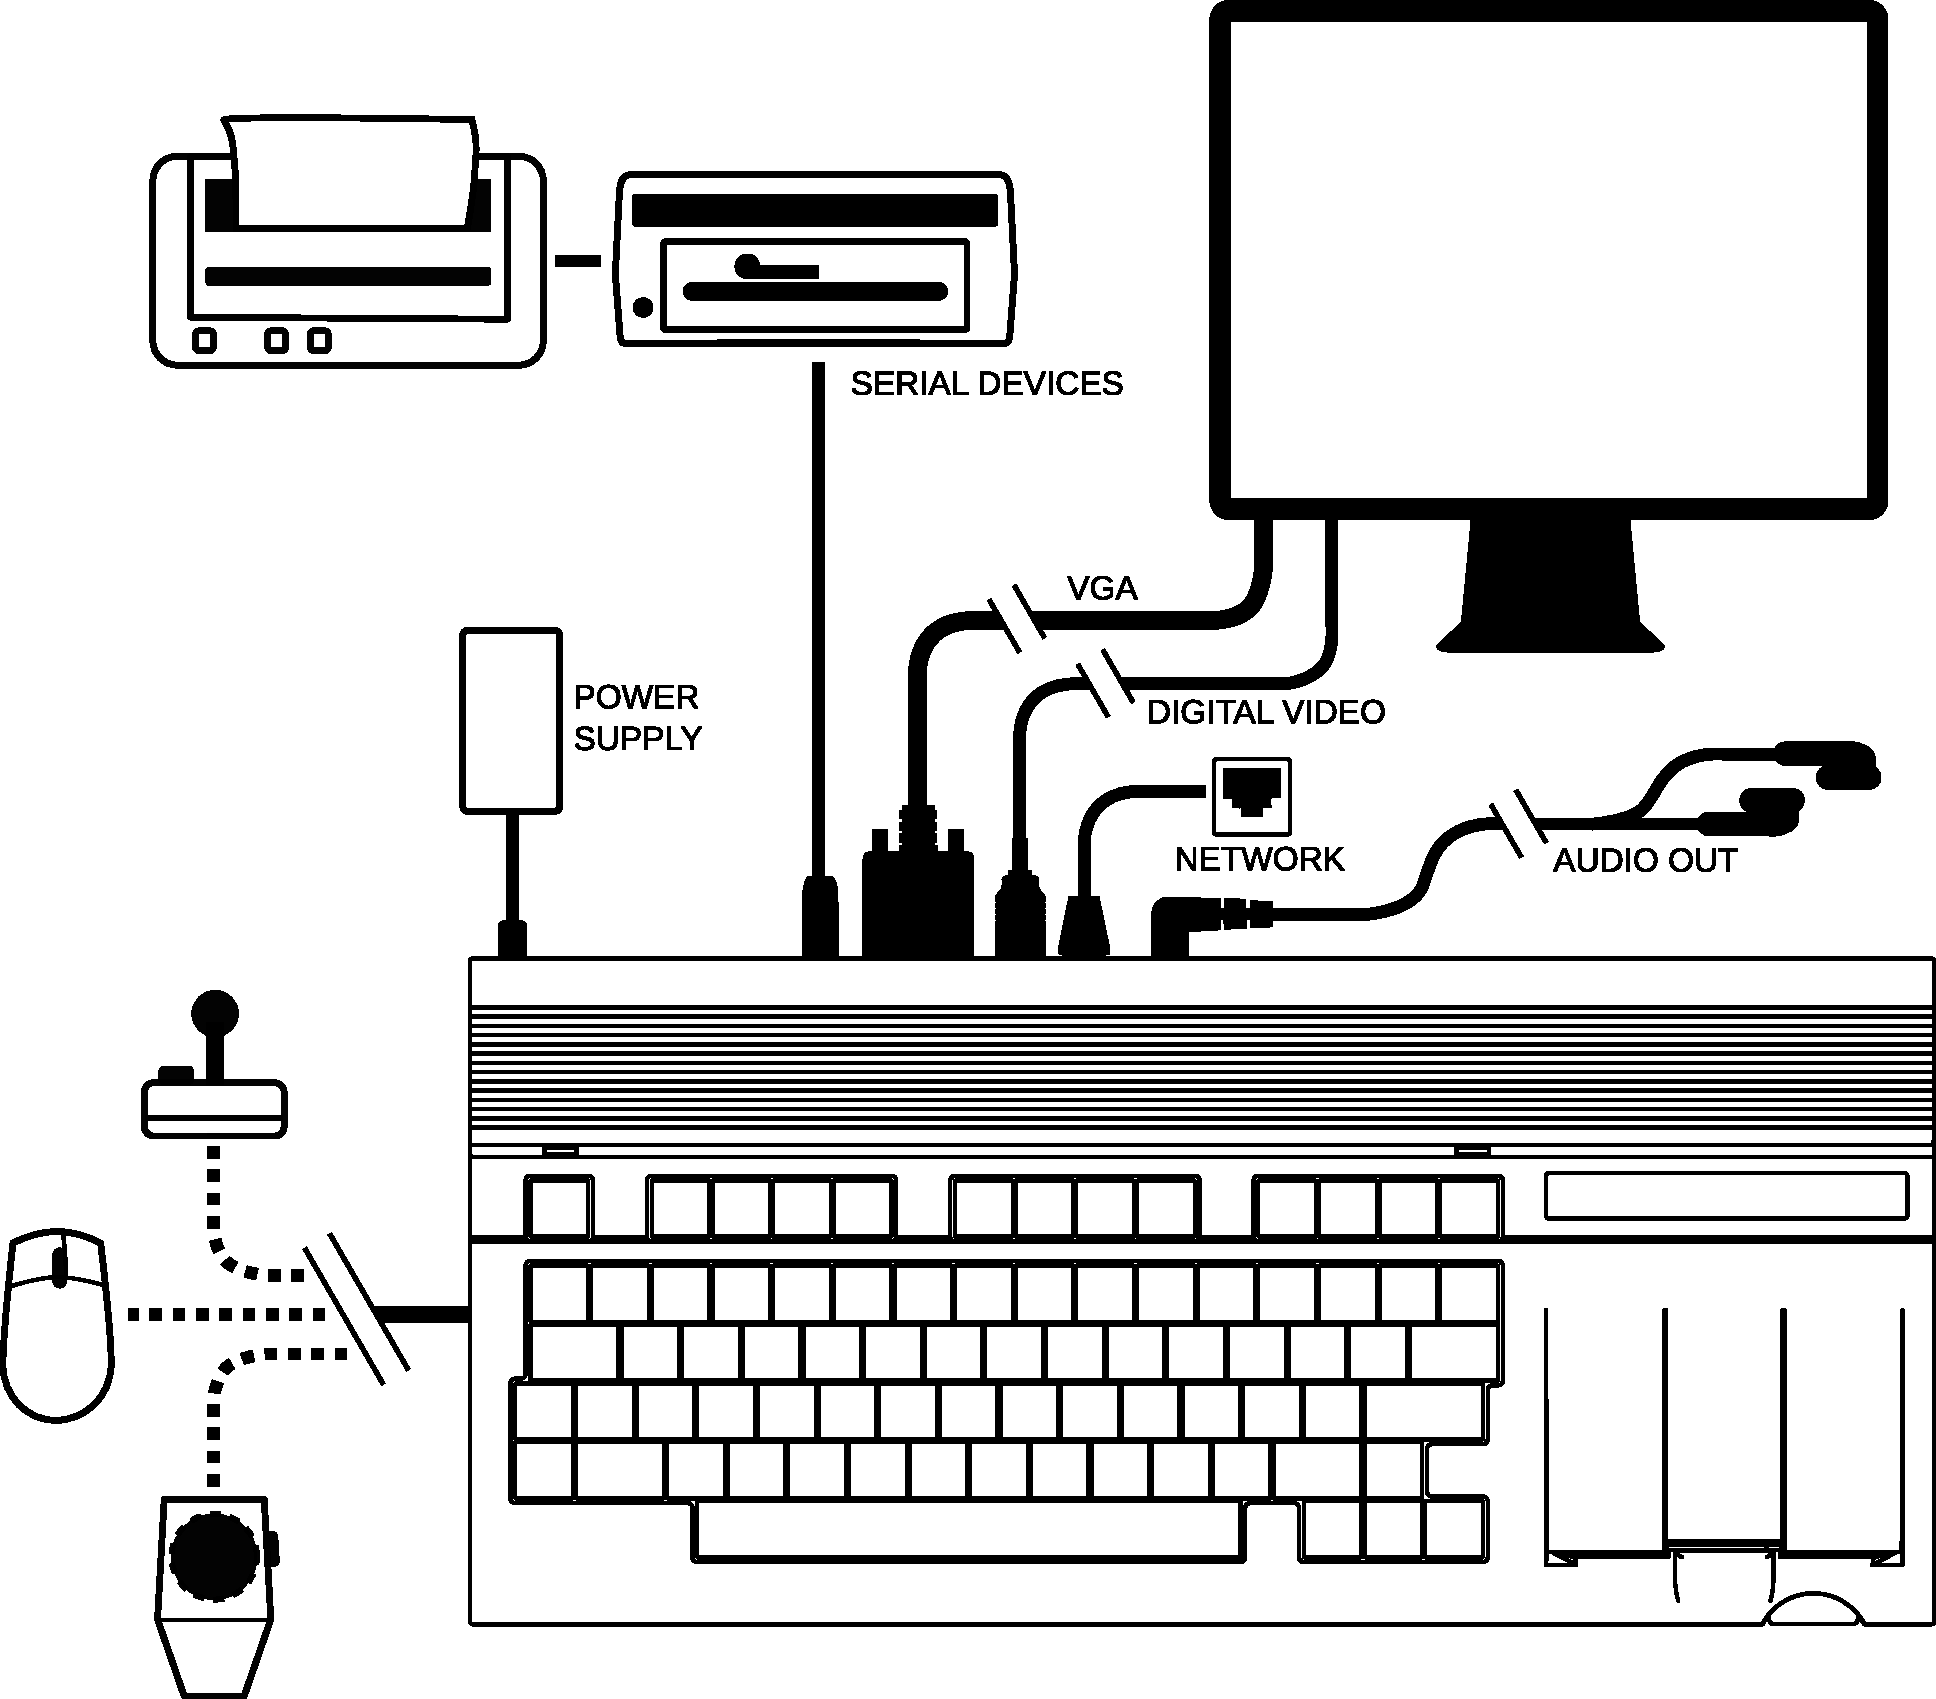
\includegraphics[width=\linewidth]{images/illustrations/mega65-top.pdf}

To connect your MEGA65 to a display:

\begin{enumerate}
	\item Connect the power supply to the power supply socket of the MEGA65.
	\item If you have a VGA monitor and a VGA cable, connect one end to the VGA port of the MEGA65 and the other end into your VGA monitor.
	\item If you have a TV or monitor with a compatible Digital Video connector, connect one end of your cable to the Digital Video port of the MEGA65, and the other into the Digital Video port of your monitor. If you own a monitor with a DVI socket, you can use a Digital Video to DVI adapter.
\end{enumerate}

\newpage
\section{Optional Connections}
\index{Connections!IEC}
\index{SD Cards!Locations}
\begin{enumerate}
	\item The MEGA65 includes an internal 3.5" floppy disk drive. You can also connect older Commodore{\textregistered} IEC serial floppy drives to the MEGA65, such as the Commodore 1541, 1571 or 1581. To use these drives, connect one end of an IEC cable to the Commodore floppy disk drive and the other end to the Disk Drive socket of the MEGA65. You can also connect SD2IEC devices and Pi1541's. It is also possible to daisy-chain additional floppy disk drives or Commodore compatible printers.
	\item You can connect your MEGA65 to an Ethernet network using a standard Ethernet cable.
	\item For enjoying audio from your MEGA65, you can connect a 3.5mm audio jack cable to an audio amplifier or speaker system. If your system has RCA connectors you will need a 3.5mm audio jack to twin RCA adapter cable. The MEGA65 also has a built-in amplifier to allow the use of headphones.
	\item A microSD card, type SDHC between 4GB and 32GB, can be inserted into the external microSD card slot at the rear of the MEGA65. For more information on using the microSD card slot, see ``Introducing SD Cards'' on page \pageref{sec:introducing-sd-cards}.
\end{enumerate}

\index{Real-Time Clock!Installing the Battery}
\subsection{Installing the Real-Time Clock Battery}

The MEGA65 includes a Real-Time Clock, which is used to display the time and date on the startup screen, to add timestamps to files that the MEGA65 writes to your SD cards, and by the {\bf DT\$} and {\bf TI\$} BASIC65 variables. This clock utilises a CR2032 coin-cell battery\footnote{Early models of MEGA65 with the "R3A" board revision used a battery of type CR1220 for the Real-Time Clock. Revisions "R5" and later, which began shipping in late 2023, use a CR2032 battery.} to keep time when the MEGA65 isn't switched on. The MEGA65 does not include a battery in order to avoid issues related to shipping batteries internationally.

To install the battery, use a Phillips-head screwdriver to open the case, exposing the motherboard. The case is held together with three screws, all of which are along the bottom of the front side of the case. Once the screws have been removed, carefully lift the top half of the case. Note the orientation of the keyboard connector, then disconnect it.

The battery is located between the controller ports and the keyboard connector.

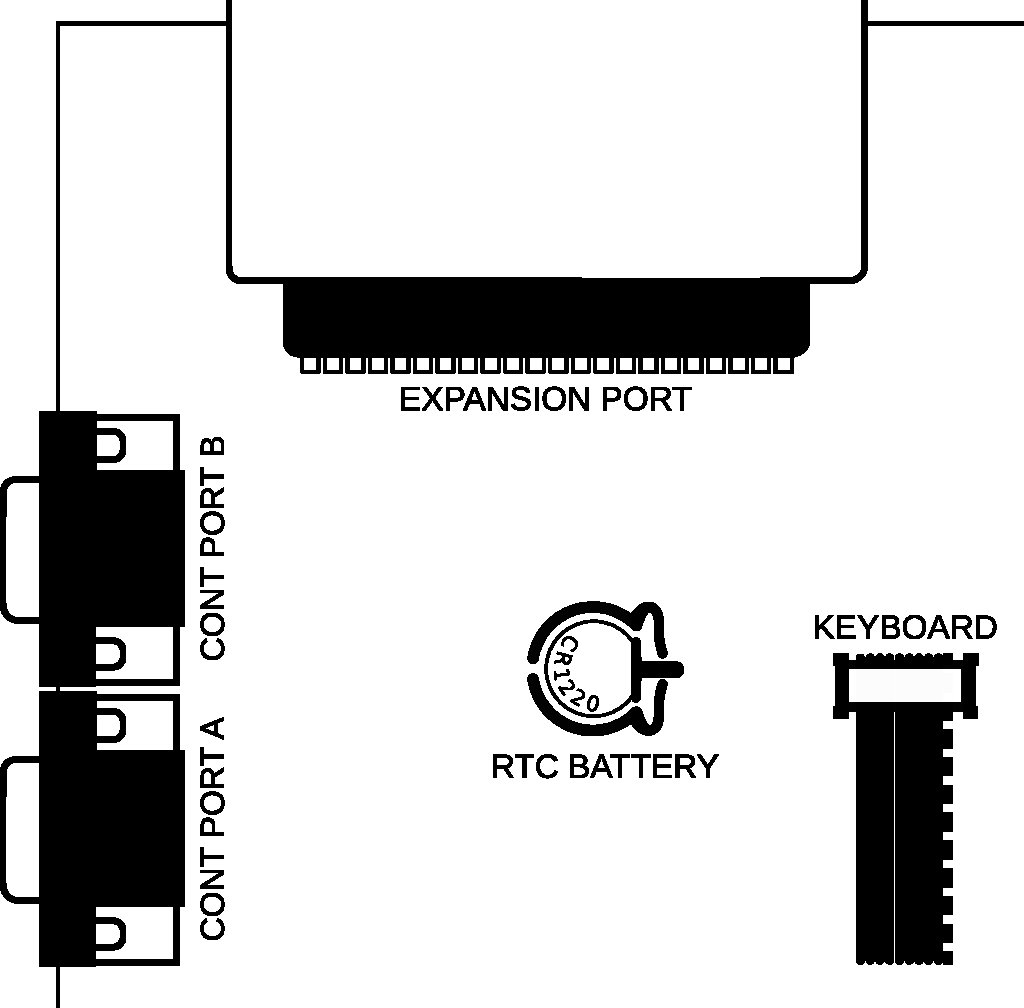
\includegraphics[width=10cm]{images/illustrations/rtc-battery-location.pdf}

If you are removing an existing battery, push the battery release lever on the bottom (flat-sided) side of the battery socket away from the battery to remove it. Insert the new battery with the side labelled {\bf +} facing up, and press it into place.

Once you have re-assembled your MEGA65, you can set the time in the Configure menu. For more information on how to set the Real-Time Clock, refer to the Configuration Utility section on page \pageref{sec:configuration-utility}.


\newpage

\section{Switching the MEGA65 on for the First Time}
\label{onboarding}

Switch the MEGA65 on using the power switch on the left-hand side of the computer.

When you switch your MEGA65 on for the first time, it displays the initial configuration (``on-boarding'') screen. You can use this screen to set the time and date on the Real-Time Clock (if you have installed the CR2032 battery), change the video display mode, and test the audio. All of these settings can be changed later.

\begin{center}
  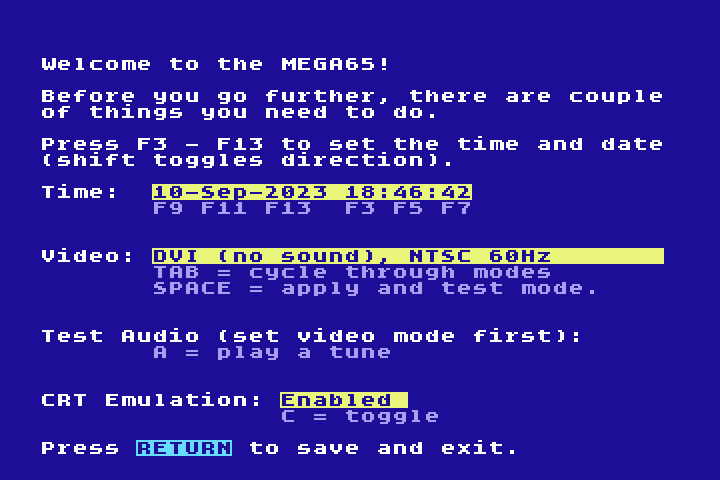
\includegraphics[trim= 10mm 15mm 10mm 10mm,clip,width=0.7\linewidth]{images/img011_final_boot_01.png}
\end{center}

For video display modes, you can select between PAL or NTSC emulation, and you can select whether your DVI display supports sound. If you are using the VGA video output, the DVI sound mode has no effect.

\underline{Note}: A DVI display that does not support sound will not work with the ``enhanced'' sound mode. With such a display, you must select a video mode with ``no sound,'' and connect a speaker to the 3.5 mm audio jack.

PAL and NTSC are analog video signal formats that affect the the resolution and vertical sync speed of the video output, even when using a modern digital display. Your display may support either mode, or it may only support one or the other. You can use this screen to test the modes with your display.

Select and test you video configuration. For example, press \specialkey{TAB} to switch to the ``PAL 50HZ'' mode.
\index{Display!Setting PAL/NTSC}
\begin{center}
  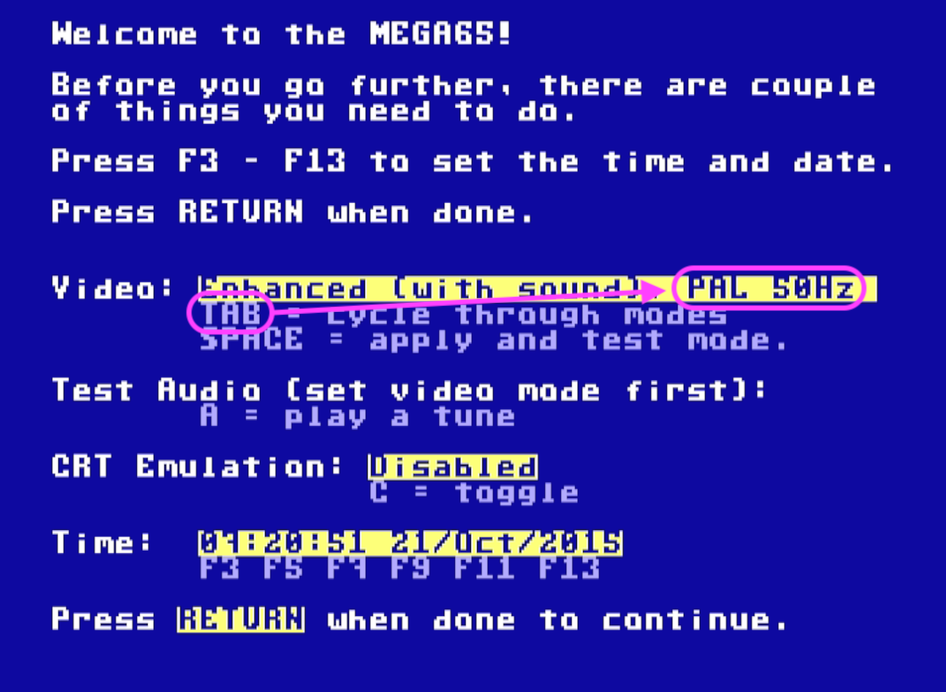
\includegraphics[width=0.7\linewidth]{images/img011_final_boot_02.png}
\end{center}

Press \megakey{SPACE} followed by \megakey{Y} to test the new video mode.

\begin{center}
  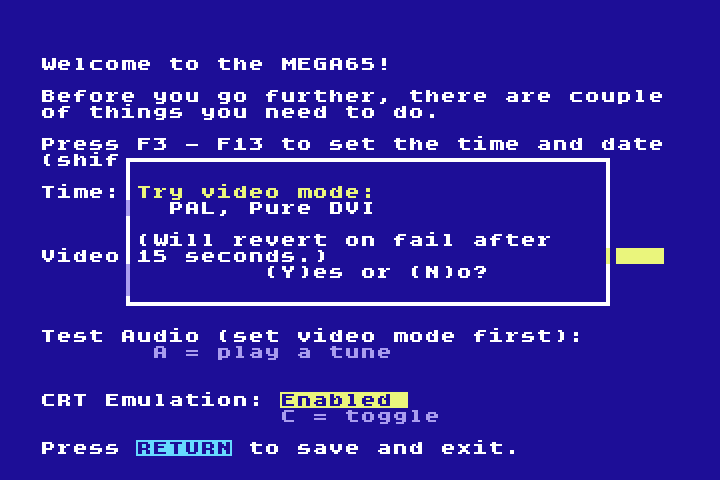
\includegraphics[trim= 15mm 10mm 10mm 15mm,clip,width=0.7\linewidth]{images/img011_final_boot_03.png}
\end{center}

Press \megakey{K} to keep the new video mode.

\begin{center}
  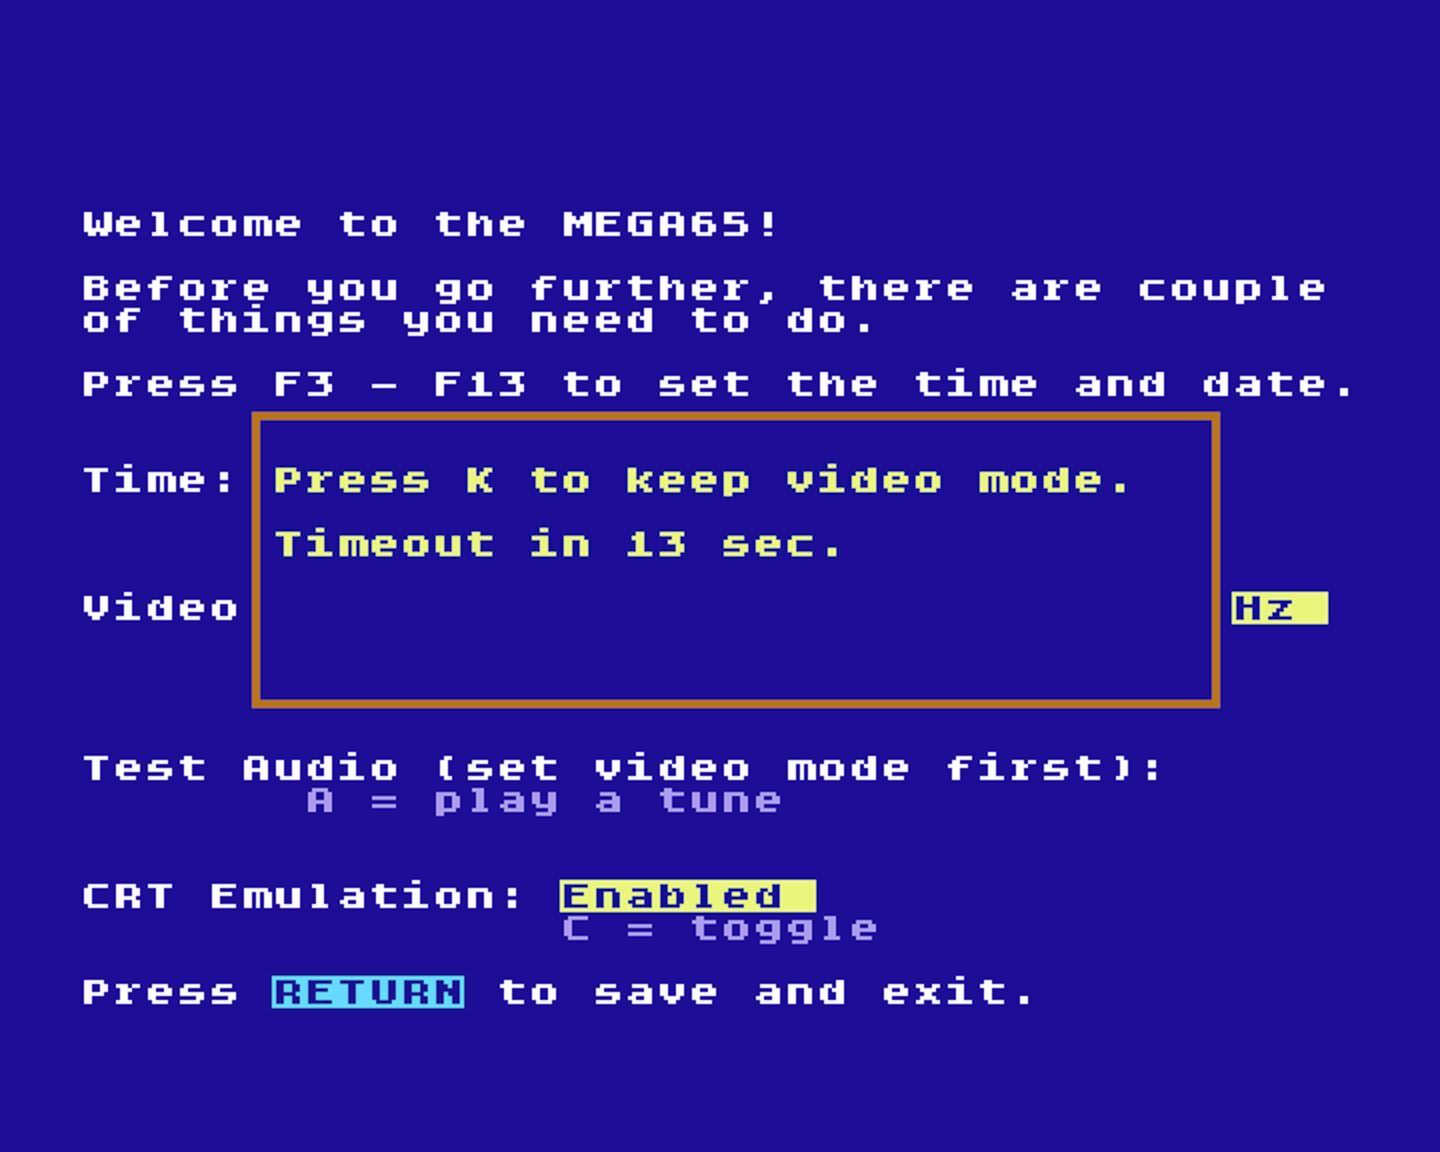
\includegraphics[trim= 20mm 20mm 10mm 25mm,clip,width=0.7\linewidth]{images/img011_final_boot_04.png}
\end{center}

Take this opportunity to test your sound set-up. Press \megakey{A} to play a sound.

The ``CRT emulation'' option is a fun choice when using a modern flat panel display. It adds vertical gaps between pixels to simulate the CRT raster line. Try it to see if you like it: press the \megakey{C} key to toggle it on and off.

Finally, press \specialkey{RETURN} to complete the configuration.

For more information about configuring your MEGA65, see chapter \vref{cha:configuringyourmega}.

\section{The Intro Disk}

After completing the on-boarding configuration, your MEGA65 starts the Intro Disk menu. The Intro Disk is a collection of software made by the MEGA65 community that demonstrates some of the capabilities of the computer. Take some time to browse the menus and try some of the demos. After each demo, press the reset button on the left-hand side of the computer to return to the Intro Disk menu.

\begin{center}
  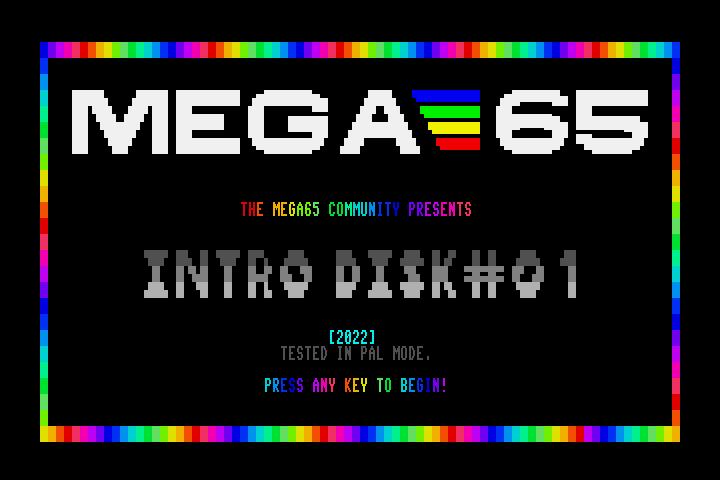
\includegraphics[width=0.7\linewidth]{images/demo_title.jpg}
\end{center}

By default, the Intro Disk menu opens each time you switch on the computer. Once you are more familiar with the MEGA65, you may wish to disable this. Press \megakey{D} at the Intro Disk menu to disable its auto-boot feature.

Press \megakey{X} to exit the Intro Disk menu and access BASIC 65. With the Intro Disk auto-boot feature disabled, the MEGA65 goes directly to BASIC 65 when you switch it on.

\begin{center}
  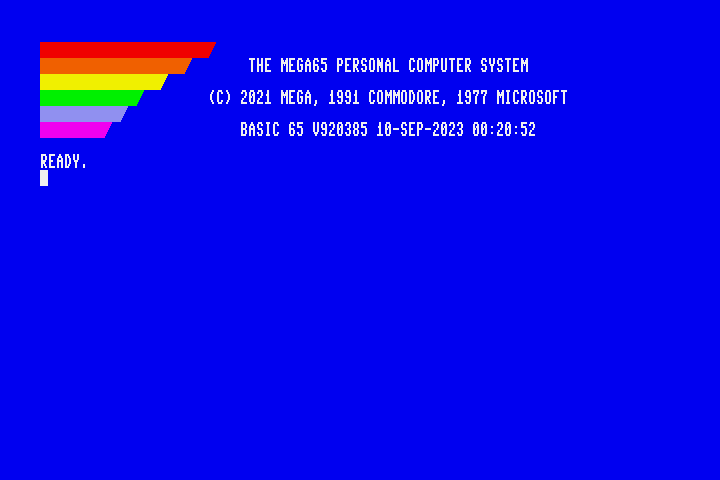
\includegraphics[trim=0 2cm 0 0,clip,width=0.7\linewidth]{images/img011_final_boot_06.png}
\end{center}

\subsection{The Cursor}

The flashing square underneath the \screentext{READY} prompt is called the cursor. The cursor indicates that the computer is ready to accept input. Pressing keys on the keyboard will print their respective characters onto the screen. The characters will be printed at the current cursor position, and the cursor will advance to the next position after every key press.

Here you can type commands, that can do things such as loading a program. You can also start entering program code!

\chapter{Getting Started}
\phantomsection
\section{Keyboard}
\label{cha:getting-started}

Now that everything is connected, it's time to get familiar with the MEGA65 keyboard.

You may notice that the keyboard is a little different from the keyboards used on computers today. While most keys will be in familiar positions, there are some specialised keys, and some with special graphic symbols marked on the front.

Here's a brief description of how some of these special keys function.

\subsection{Command Keys}

The Command Keys are: \specialkey{RETURN}, \specialkey{SHIFT}, \specialkey{CTRL}, \megasymbolkey, and \widekey{RESTORE}.

\subsubsection{RETURN}

Pressing \specialkey{RETURN} enters the information you have typed into the MEGA65's memory. The computer will either act on a command, store some information, or display an error message if you made a mistake.

\subsubsection{SHIFT}

The two \specialkey{SHIFT} keys are located on the left and the right. They work very much like the Shift key on a regular keyboard, however they also perform some special functions as well.

In upper case mode, holding down \specialkey{SHIFT} and pressing any key with two graphic symbols on the front prints the right-most graphic symbol to the screen. For example, \specialkey{SHIFT} and \megakey{J} prints the \graphicsymbol{J} character.

In lower case mode, pressing \specialkey{SHIFT} and a letter key prints the upper case letter on that key.

Finally, holding \specialkey{SHIFT} down and pressing a Function key accesses the function shown on the front of that key. For example: \specialkey{SHIFT} and \megakey{F1} activates \textbf{F2}.


\subsubsection{SHIFT LOCK}

In addition to \specialkey{SHIFT} is \specialkey{SHIFT\\LOCK}. Press this key to lock down the Shift function. Now any key you press while \specialkey{SHIFT\\LOCK} is illuminated prints the character to the screen as if you were holding down \specialkey{SHIFT}. This includes special graphic characters.

\subsubsection{CTRL}

\specialkey{CTRL} is the Control key. Holding down \specialkey{CTRL} and pressing another key allows you to perform Control Functions. For example, holding down \specialkey{CTRL} and one of the number keys allows you to change text colours. The colour that is printed at the top row on the front of the number key will be used.

There are some examples of this in \bookvref{sec:screen-editor}, and all of the Control Functions are listed in \bookvref{appendix:controlcodes}.

If a program is being LISTed to the screen, holding down \specialkey{CTRL} slows down the display of each line.

Holding \specialkey{CTRL} and pressing \megakey{*} enters the Matrix Mode Debugger (refer to the {\bf MEGA65 Book} for more details).

\subsubsection{RUN STOP}

Normally, pressing \specialkey{RUN STOP} stops the execution of a program. Holding \specialkey{SHIFT} while pressing \specialkey{RUN STOP} loads the first program from disk.

Programs are able to disable \specialkey{RUN STOP}.

You can boot your MEGA65 into the Machine Code Monitor by holding down \specialkey{RUN STOP} and pressing reset on the left-hand side.

\subsubsection{RESTORE}

The computer screen can be restored to a clean state without clearing the memory by holding down \specialkey{RUN STOP} and pressing \widekey{RESTORE}. This combination also resets operating system vectors and re-initialises the screen editor, which makes it a handy combination if the computer has become a little confused.

Programs are able to disable this key combination.

You can also enter the Freeze Menu by holding \widekey{RESTORE} down for more than one second. From there you can access the Machine Code Monitor.

\newpage

\subsubsection{THE CURSOR KEYS}

At the bottom right-hand side of the keyboard are the cursor keys. These four directional keys allow you move the cursor to any position for on-screen editing.

The cursor moves in the direction indicated on the keys: \megakey{$\leftarrow$} \megakey{$\uparrow$} \megakey{$\rightarrow$} \megakey{$\downarrow$}.

However, it is also possible to move the cursor up by using \specialkey{SHIFT} and \megakey{$\downarrow$}. In the same way you can move the cursor left by using \specialkey{SHIFT} and \megakey{$\rightarrow$}.

You don't have to keep pressing a cursor key over and over. If you need to move the cursor a long way, you can keep the key pressed down. When you are finished, simply release the key.

\subsubsection{INSerT/DELete}

This is the INSERT / DELETE key. When pressing \specialkey{INST\\DEL}, the character to the left is deleted, and all characters to the right are shifted one position to the left.

To insert a character, hold \specialkey{SHIFT} and press \specialkey{INST\\DEL}. All the characters to the right of the cursor are shifted to the right. This allows you to type a letter, number or any other character at the newly inserted space.


\subsubsection{CLeaR/HOME}

Pressing \specialkey{CLR\\HOME} places the cursor at the top left-most position of the screen.

Holding down \specialkey{SHIFT} and pressing \specialkey{CLR\\HOME} clears the entire screen {\it and} places the cursor at the top left-most position of the screen.

\subsubsection{MEGA KEY}

\megasymbolkey or the MEGA key provides a number of different functions and can be used to launch special utilities.

Holding \specialkey{SHIFT} and pressing \megasymbolkey switches between lower and uppercase character modes.

Holding \megasymbolkey and pressing any key with two graphic symbols on the front prints the left-most graphic symbol to the screen.

Holding \megasymbolkey and pressing any key that shows a single graphic symbol on the front prints that graphic symbol to the screen.

Holding \megasymbolkey and pressing a number key switches to one of the colours in the second range, i.e., the colour that is printed at the bottom row on the front of the number key will be used.

Holding \megasymbolkey and pressing \specialkey{TAB} enters the Matrix Mode Debugger (refer to the {\bf MEGA65 Book} for more details).

Switching on the MEGA65 or pressing the reset button on the left-hand side while holding down \megasymbolkey switches the MEGA65 into C64-mode.

\subsubsection{NO SCROLL}
If a program is being LISTed to the screen, pressing \specialkey{NO\\SCROLL} freezes the screen output. This feature is not available in C64-mode.


\subsection{Function Keys}

There are seven Function keys available for use by software applications. \megakey{F1} \megakey{F3} \megakey{F5} \megakey{F7} \megakey{F9} \megakey{F11} and \megakey{F13} can be used to perform specific functions with a single press.

Hold \specialkey{SHIFT} to access \megakey{F2} through to \megakey{F14} as shown on the front of each Function key.

Only Function keys \megakey{F1} to \megakey{F8} are available in C64-mode.

\subsubsection{HELP}

\specialkey{HELP} can be used by software and also acts as \megakey{F15} / \megakey{F16}.

\subsubsection{ALT}

Holding \specialkey{ALT} down while pressing other keys can be used by software to perform specific functions. Not available in C64-mode.

Holding \specialkey{ALT} down while switching the MEGA65 on activates the Utility Menu. You can format an SD card, or enter the MEGA65 Configuration Utility to select the default video mode and change other settings, or to test your keyboard.

\subsubsection{CAPS LOCK}

\specialkey{CAPS\\LOCK} works similarly to \specialkey{SHIFT\\LOCK} in C65 and MEGA65-modes, but only modifies the letter keys.
Also, holding \specialkey{CAPS\\LOCK} down forces the processor to run at the maximum speed. This can be used, for example,
to speed up loading from the internal disk drive or SD card, or to greatly speed up the de-packing process after a program is run.
This can reduce the loading and de-packing time from many seconds to as little as a fraction of a second.

\section{The Screen Editor}
\label{sec:screen-editor}

When your turn on your MEGA65 or reset it, the following screen will appear:

\begin{center}
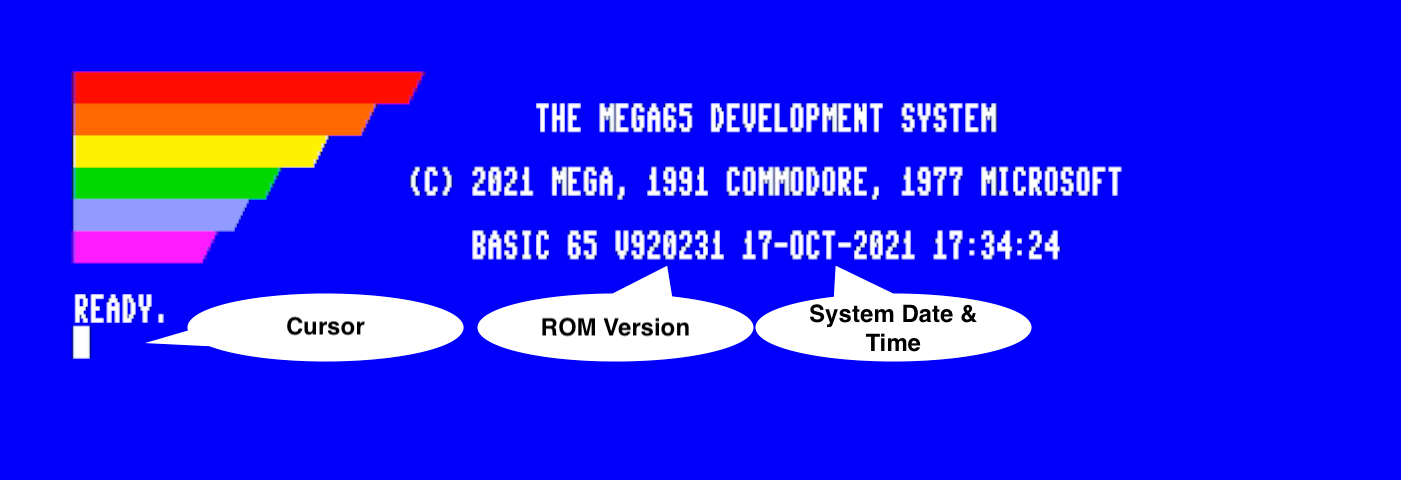
\includegraphics[width={10cm}]{images/introduction-screen/layout.png}
\end{center}

The colour bars in the top left hand of the screen can be used as a guide to help calibrate the colours of your display. The screen also displays the name of the system, the copyright notice, and the version of BASIC that is contained in Read-only memory.

Also displayed is the type of keyboard, and whether there is any additional hardware present, such as a RAM expansion.

Finally, you will see the READY prompt and the flashing cursor.

You can begin typing keys on the keyboard and the characters will be printed at the cursor position. The cursor itself will advance after each key press.

You can also produce reverse text or colour bars by holding down the \megakey{CTRL} key and pressing the \megakey{9} key, or the \megakey{R} key. This enters reverse text mode.
When this is enabled, you can press and hold the \megakey{Space bar}. While doing so, a white bar will be drawn across the screen.

You can even change the current colour by holding the \megakey{CTRL} key down and pressing a number key (from \megakey{1} to \megakey{8}). For example, if you press and hold the \megakey{CTRL} key, and press \megakey{1}, the colour will change to black. Now, when you hold down the \megakey{Space bar}, a black bar will be drawn. If you continue to change the colour and press the \megakey{Space bar}, you will get an effect similar to the image below:


\begin{center}
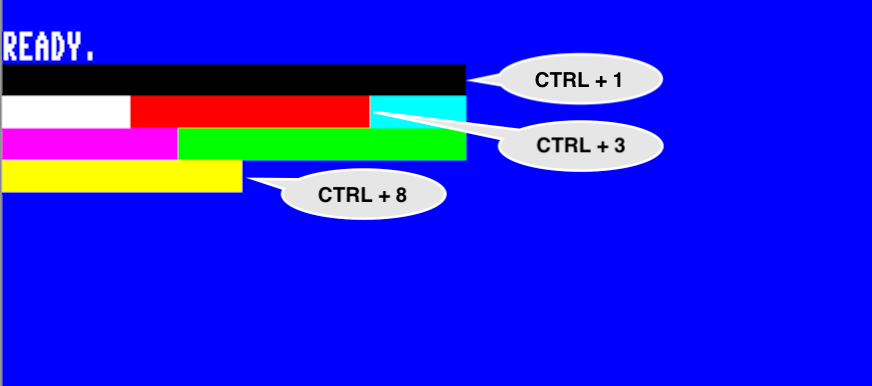
\includegraphics[width={10cm}]{images/introduction-screen/colour-bars.png}
\end{center}


You can disable the reverse text mode by holding \megakey{CTRL} and pressing the \megakey{0} key.

By pressing any keys, the characters will be typed out in the chosen colour.

There are a further eight colours available via the \megasymbolkey key. Hold the \megasymbolkey key and press a key from \megakey{1} to \megakey{8} to change to one of the secondary colours. The colour that is printed at the bottom row on the front of the number key will be used. For example, if you held the \megasymbolkey key down while pressing \megakey{4}, dark green will be used. For even more colours, see \bookvref{appendix:escapesequences}.

\needspace{4cm}
You can create fun pictures just by using these colours and letters.  Here's an example of what a year four student drew:

\begin{center}
\includegraphics[width={6cm}]{images/caleb-PETSCII-TNT-final}
\end{center}

What will you draw?

\needspace{2cm}
\textbf{Functions}

Functions using the \megakey{CTRL} key are called \textbf{Control Functions}.
Functions using the \megasymbolkey key are called \textbf{Mega Functions}. There are also functions called by using the \megakey{Shift} key. These are (not surprisingly) called \textbf{Shift Functions}.

Lastly, using the \megakey{ESC} key are \textbf{Escape Sequences}.

\needspace{2cm}
\textbf{ESC Sequences}

Escape sequences are performed a little differently than a Control function or a Shifted function. Instead of holding the modifier key down, an Escape sequence is performed by pressing the \megakey{ESC} key and releasing it, followed by pressing the desired key code.

For example: to switch between 40/80 column mode, press and release the \megakey{ESC} key. Then press the \megakey{X} key.

You can see all of the available escape sequences in \bookvref{appendix:escapesequences}, but some are shown in this section.

There are more modes available. You can create flashing text by holding the \megakey{CTRL} key and pressing the \megakey{O} key. Any characters you press will flash. Turn flash mode off by pressing \megakey{ESC} then \megakey{O}.



\section{Editor Functionality}


The MEGA65 screen can allow you to do advanced tabbing, and moving quickly around the screen in many ways to help you to be more productive.

Press the \megakey{Home} key to go to the home position on the screen. Hold the \megakey{CTRL} key down and press the \megakey{W} key several times. This is the \textbf{Word Advance function} which jumps your cursor to the next word, or printable character.

You can set custom tab positions on the screen for your convenience. Press \megakey{Home} and then \megakey{$\rightarrow$} to the fourth column. Hold down \megakey{CTRL} and press the \megakey{X} key to set a tab. Move another 20 positions to the right again, and do \megakey{CTRL} and \megakey{X} again to set a second tab.

Press the \megakey{Home} key to go back to the home position. Hold the \megakey{CTRL} key and press the \megakey{I} key. This is the \textbf{Forward Tab function}. Your cursor will tab to the fourth position. Press \megakey{CTRL} and \megakey{I} again. Your cursor will move to position 8. Why? By default, every 8th position is already set as a tabbed position. So the 4th and 20th positions have been added to the existing tab positions. You can continue to press the \megakey{CTRL} and \megakey{I} keys to the 16th and 20th positions.

To find the complete set of Control codes, see \bookvref{appendix:controlcodes}.


\newpage



\textbf{Creating a Window}

You can set a window on the MEGA65 working screen. Move your cursor to the beginning of the "BASIC 65" text. Press \megakey{ESC}, then press \megakey{T}. Move the cursor 10 lines down and 15 to the right.

Press the \megakey{ESC} key, then \megakey{B}. Anything you type will be contained within this window.

To escape from the window back to the full screen, press the \megakey{Home} key twice.


\textbf{Extras}

Long press on \megakey{Restore} to go into the Freeze Menu.  Then press \megakey{J} to switch joystick ports without having to physically swap the joystick to the other port.

Go to \textbf{Fast mode} with poke 0, 65 or use the freeze menu.

\megakey{MEGA} and \megakey{Shift} switches between text uppercase and lowercase for the entire display.

\chapter{Configuring your MEGA65}
\label{cha:configuring}

\section{Important Note}

For your convenience, your MEGA65 comes with an SD card with all of the essential
files already on it, so you may prefer to skip this section and jump straight to
the on-boarding section on page \pageref{onboarding}.

Alternatively, you're welcome to read this section and familiarise
yourself on how your SD card was prepared.

{\bf Do not format the SD card that came with your MEGA65}.
If you want to create a new bootable SD card, please use another one,
and keep the SD card that came with your MEGA65 as a safety backup.

\section{Formatting SD cards}
\index{SD Cards!Formatting}
The MEGA65 has two SD card slots: A full-size SD card slot inside, under
the trap-door, and a microSD size slot on the rear.  The current version
of the MEGA65 firmware only supports the use of one SD card at a time.
If you have cards in both slots, the MEGA65 will default to the external slot. The exception to this is that the MEGA65's FDISK/FORMAT
utility can access both, allowing you to select which SD card to format or
repair.

If you wish to use a different SD card to the pre-configured one supplied with your MEGA65, the new SD card must be formatted first.

{\bf This must be done on the MEGA65, not on a PC or other computer.}

{\em Only use SDHC cards. Older SD cards (typically with
  a capacity of <4GB) will not work. Newer SDXC cards with
  capacities greater than 32GB may or may not work. We would
  appreciate hearing your experience with such cards. It is unimportant
  as to which file-system is currently on the card, as the MEGA65
  FDISK/FORMAT utility will completely reformat the card.}

There are several reasons for this: First, to fit the most
features into the MEGA65's small operating system, it is
particular about the FAT32 file system it uses. Second, only the
MEGA65 FDISK/FORMAT utility can create a MEGA65 System Partition. The
MEGA65 System Partition holds non-volatile configuration settings for
your MEGA65, and also contains the freeze slots that make it easy to
switch between MEGA65 programs and games.

Formatting an SD card on the MEGA65 is easy. Switch the MEGA65 on while holding \specialkey{ALT} down.

This will present the MEGA65 Utility Menu, which contains a
selection of built-in utilities, similar to the following:

%\begin{wrapfigure}{l}{0.7\textwidth}
\begin{center}
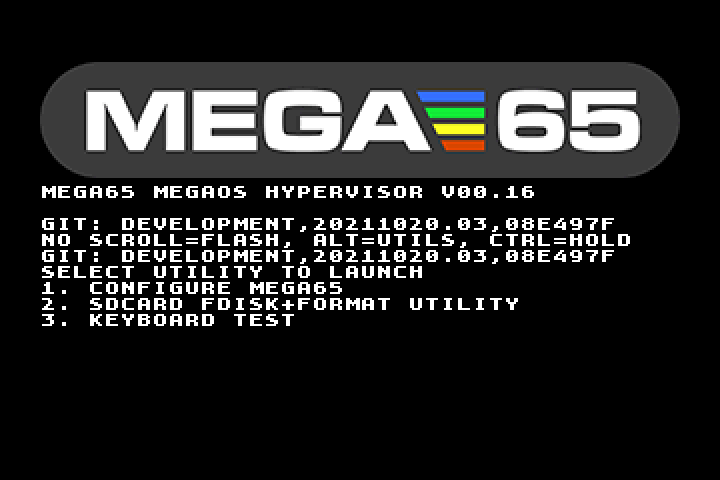
\includegraphics[width=0.7\textwidth]{images/ss-utilmenu.png}
\end{center}
%\end{wrapfigure}

Note that the Utility Menu is always accessible, even if no SD card is present in both the internal and external slots.

The exact set of utilities
depends on the model of your MEGA65 and the version of the MEGA65
factory core which it is running. However, all versions include both
the MEGA65 FDISK/FORMAT utility (which is called \screentext{SDCARD FDISK+FORMAT UTILITY} in the screenshot above),
and the MEGA65 Configure utility.
Most models also include a keyboard test utility, that you can use
to test that your keyboard is functioning correctly.  This is
the same utility used in the factory when testing brand
new keyboards.

Select the number that corresponds to the FDISK/FORMAT utility.  This
will typically be 2.  The FDISK utility will start, and attempt to
detect the size of all SD cards you have installed.  If you have both
an internal and external SD card installed, it will allow you to
choose which one you wish to format. The internal SD card is bus 0,
and the external microSD card is bus 1. Note that the MEGA65 will
always attempt to boot from the external microSD card if one is
present.

For safety, when formatting we {\em strongly} recommend
that you remove any SD card or microSD card that you do not intend to
format, so that you do not accidentally destroy any data.  This is
because formatting an SD card on the MEGA65 cannot be undone, and
all data currently on the SD card {\em will be lost}.  If you
have files or data on the SD card that you wish to retain, you
should first back them up.  The contents of the FAT32
partition can be easily backed up by inserting the SD card into
another computer.  The contents of the MEGA65 System Partition,
including the contents of freeze slots requires the use of specialised
software.

You should aim to back up valuable data from your
MEGA65 on a regular basis, especially while the computer remains under
development.  While we take every care to avoid data corruption or
other mishaps, we cannot guarantee that the MEGA65 is free of bugs in
this regard.

If you have only an internal SD card, you might see a
display similar to the following:

\begin{center}
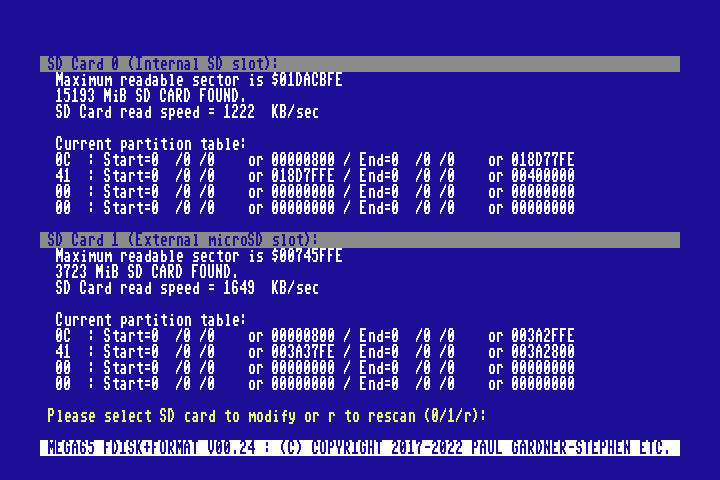
\includegraphics[trim= 10mm  7mm 10mm 10mm,clip,width=0.7\linewidth]{images/ss-m65fdisk-busselect.png}
\end{center}

Once you have selected the bus, the FDISK/FORMAT utility will ask you to confirm that you wish to delete everything:

\begin{center}
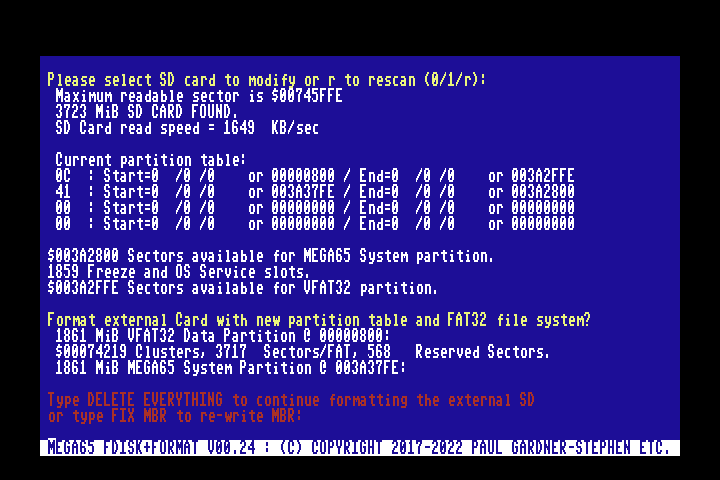
\includegraphics[trim= 10mm  7mm 10mm 15mm,clip,width=0.7\linewidth]{images/ss-m65fdisk-typesomething.png}
\end{center}

To avoid accidental loss of data, you must type \screentext{DELETE EVERYTHING} in capitals and press \specialkey{RETURN}. Alternatively, switch the MEGA65 off and on to abort this process without causing damage to your data.

It is also possible to attempt a recovery from a lost Master Boot Record error (also known as the Boot Sector), by typing \screentext{FIX MBR} instead.

The aim here is to have a correctly formatted SD card with all of the essential files stored on it so the MEGA65 can properly boot.
When switching on, the MEGA65 will search for, and boot using these files:
\begin{itemize}
\item {\tt FREEZER.M65} (Freeze Menu program)
\item {\tt AUDIOMIX.M65} (Freeze Menu audio mixer utility)
\item {\tt C64THUMB.M65} (C64 thumbnail image used in freezer)
\item {\tt C65THUMB.M65} (C65 thumbnail image used in freezer)
\item {\tt MEGA65.ROM}   (128KB ROM file)
\item {\tt MEGA65.D81} (Disk image)
\end{itemize}

Straight out of the box, the MEGA65 will only have one SD card installed, accessible via the trap-door under the case. This SD card contains all of the essential files needed to properly boot up.
If an external microSD card is also detected during boot up, the MEGA65 will give it higher priority, and will try to boot from it instead.
This means that the external microSD card needs to have the essential files on it, otherwise the MEGA65 will not boot up properly and will fall back to loading the OpenROM, which does not support all MEGA65 features.
In general, if your MEGA65 cannot boot properly and falls back to OpenROM, your boot-up screen will look similar to this:

\begin{center}
\includegraphics[trim=0 8cm 0 0,clip,width=0.7\linewidth]{images/mega65_OpenROM_boot_noSD.png}
\end{center}


\section{Installing ROM and Other Support Files}
\label{sec:installingrometc}

The MEGA65 FDISK/FORMAT utility will add a copy of the Open ROMs project's C64-compatible ROM
to your SD card, and will name it {\tt MEGA65.ROM}.

For MEGA65 owners, we have replaced this file with the latest ROM from the 'Closed ROMs'
project. It provides many improvements over the original/incomplete C65 ROMs. It contains
the operating system, BASIC 65, CBDOS and the machine language monitor BSMON.
This ROM is developed especially for the MEGA65 and can be
identified by the version number \screentext{92XXXX}.

However, you may have other ROMs that you wish to
use on your MEGA65.
You can copy as many of these as you wish onto the
SD card, just make sure that they have the {\tt .ROM} file extension.  The default ROM
should be called "{\tt MEGA65.ROM}". These files
must be 128KB in size, and use the same internal format as the ROMs
intended for the C65.  This means that the C64-mode KERNAL must be
placed at offset \$E000, a C65-mode BASIC at \$A000, and a suitable
character set at \$D000.

You can optionally name your alternate ROMs as {\tt MEGA65x.ROM}, replacing {\tt x} with a number from 0 to 9.
This allows you to quickly boot-up to your alternate ROMs by holding down a number from \megakey{0} to \megakey{9} prior
to switching on your MEGA65.

Other important support files include {\tt FREEZER.M65} and {\tt AUDIOMIX.M65}, which
allow you to use the MEGA65's integrated Freezer. More details are provided in the
'Floppy Disks, D81 Images, and the Freezer' chapter on page \pageref{cha:freezer}.

\subsection{ROM File}

\textbf{Original C65 ROMs}

You may want to source your own C65 ROM via other means.
There were many different versions created during the development of the Commodore 65,
and the MEGA65 can use any of them.  However, they will not support the advanced
features of the MEGA65, and are incomplete and buggy, as development on them ceased
due to Commodore abandoning the C65 project.

\textbf{MEGA65 Closed ROMs}

There are newer versions of the MEGA65 Closed ROM under development. These ROMs improve upon the original C65 ROMs and make better use of the extra hardware capabilities that the MEGA65 has over the original C65 hardware. These ROMs are available via the filehost (\url{https://files.mega65.org}), but only to owners of the MEGA65, who will need to login to the filehost with their credentials in order to download it. It can be located by visiting the \textbf{Files} tab and searching for "\textbf{kernal rom}":

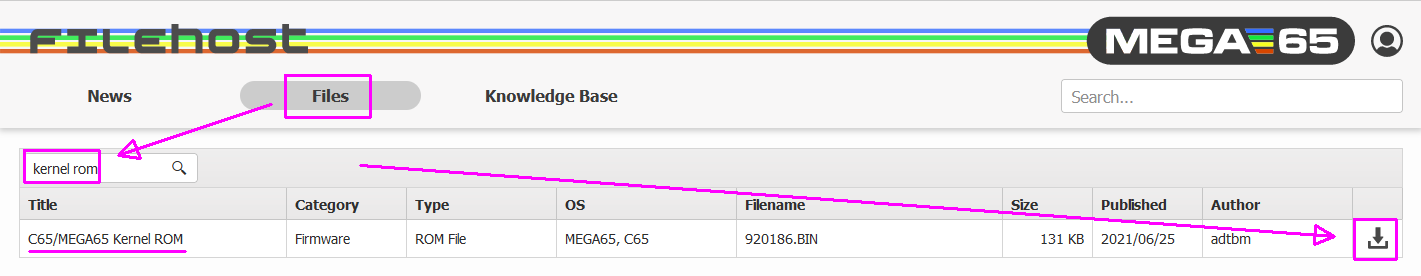
\includegraphics[width=\linewidth]{images/latest_closed_rom.png}

\textbf{MEGA65 ROM diff files}

If you have sourced your own {\tt 911001.bin} C65 ROM and would like to patch it to the latest MEGA65 closed ROM,
we do provide patches, as the additional improvements we have made to the closed rom are open source.
These diff files are available at \url{http://mega65.org/rom-diffs}

\textbf{MEGA65 Open ROMs}

Another available option is to make use of \textbf{MEGA65 Open ROMs}. The latest version of this is always downloadable from either of the following urls:

\begin{itemize}
  \item \url{http://mega65.org/open-roms}
  \item \url{https://github.com/MEGA65/open-roms/raw/master/bin/mega65.rom}
\end{itemize}


\subsection{Support Files}

For official owners of the MEGA65 (both the devkit and the final product), visit the following url and log in with the user credentials you have been provided. This will take you to the MEGA65 Filehost location where the \textbf{MEGA65 SD card essentials} download page is located. Click the \textbf{Download} link to retrieve the latest \textbf{SD essentials.rar} file.

\url{http://mega65.org/sdcard-files}

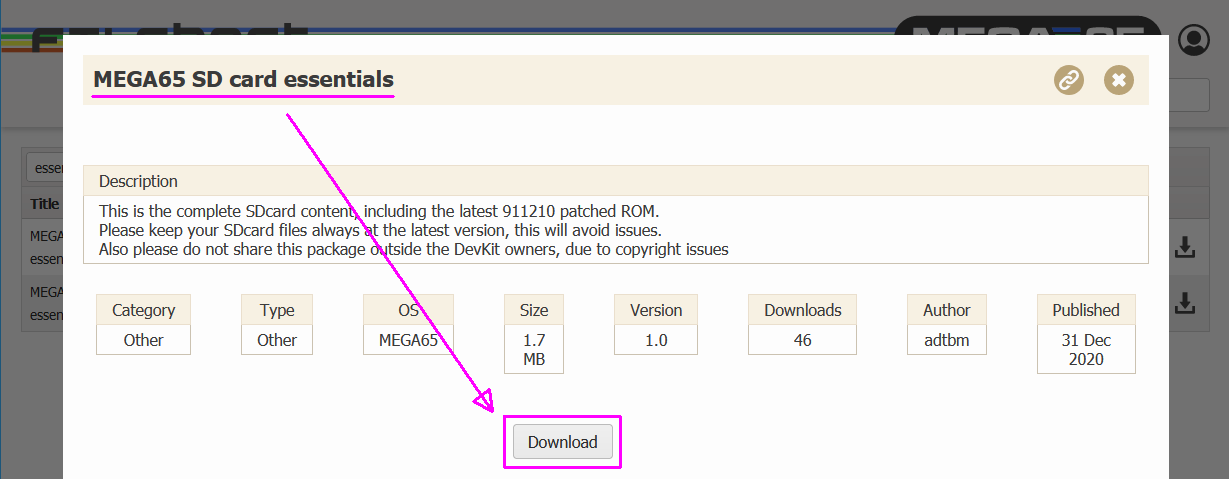
\includegraphics[width=\linewidth]{images/latest_support_files_with_closedrom.png}

Note that this link is only available to official owners of the MEGA65 product, as the fileset also contains the licensed closed-source {\tt MEGA65.ROM} file.
\ifdefined\printmanual
\else
For Nexys board owners in search of a similar fileset (without the ROM), visit the following url instead: \url{http://mega65.org/sdcard-norom}
\fi

This will take you to the MEGA65 Filehost location where the \textbf{MEGA65 SD card essentials - No ROM} download page is located. Click the \textbf{Download} link to retrieve the latest \textbf{SD essentialsNoROM.rar} file.

Note that while this fileset does not contain a ROM, there are future plans for it to include the freely available ROM from the Open ROMs project.

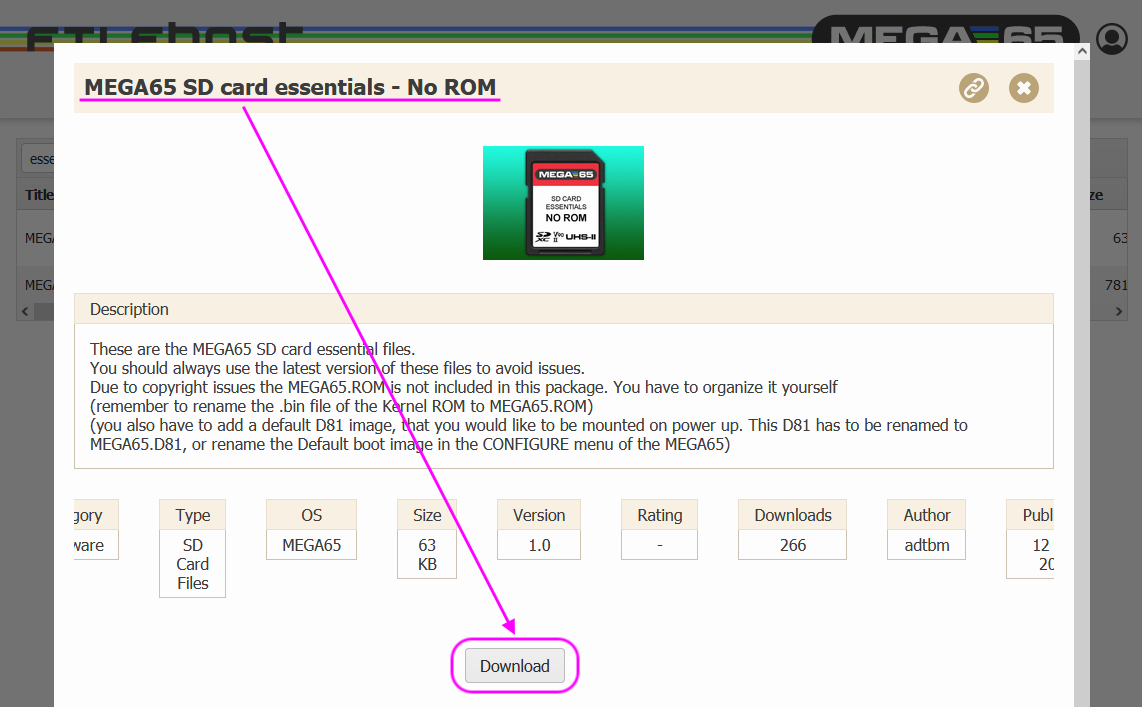
\includegraphics[width=\linewidth]{images/latest_support_files.png}

\section{On-boarding}
\label{onboarding}

On first launch of your MEGA65, you will see the on-boarding screen:

\begin{center}
  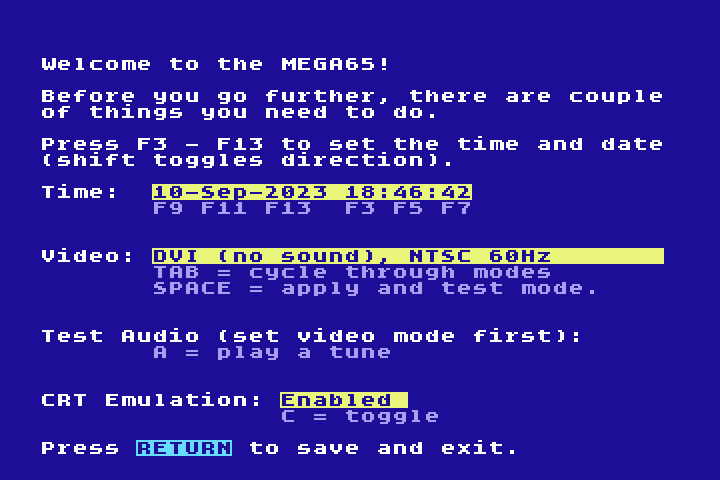
\includegraphics[trim= 10mm 15mm 10mm 10mm,clip,width=0.7\linewidth]{images/img011_final_boot_01.png}
\end{center}

Here you can select and test you screen configuration.

For example, press \specialkey{TAB} to switch to PAL 50HZ:
\index{Display!Setting PAL/NTSC}
\begin{center}
  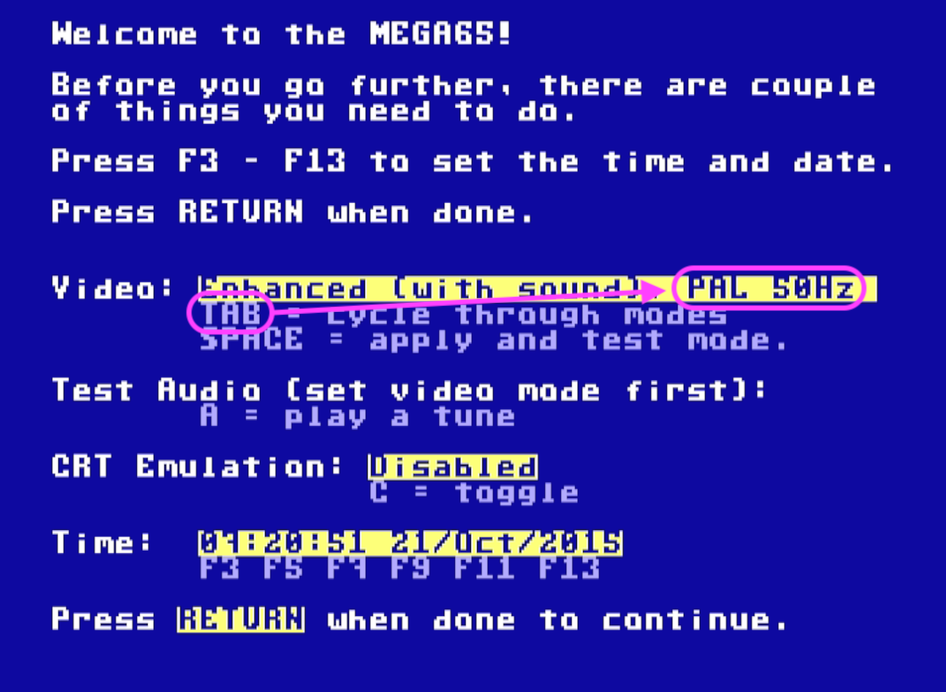
\includegraphics[width=0.7\linewidth]{images/img011_final_boot_02.png}
\end{center}

Then press \specialkey{RETURN} , followed by \megakey{Y} to test the new video mode:

\begin{center}
  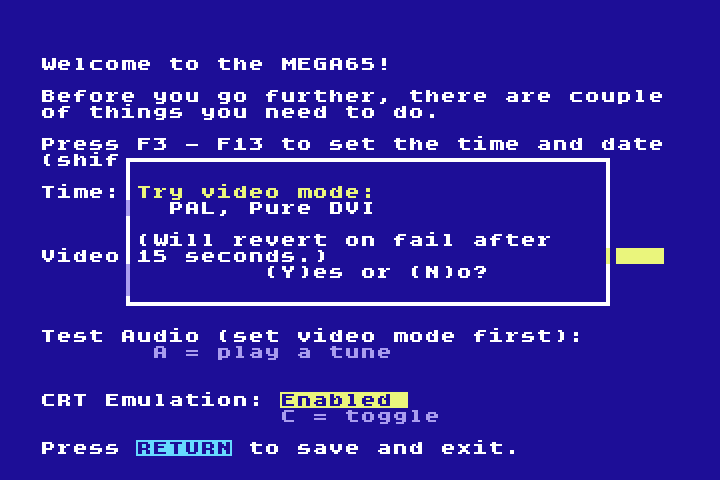
\includegraphics[trim= 15mm 10mm 10mm 15mm,clip,width=0.7\linewidth]{images/img011_final_boot_03.png}
\end{center}

Press \megakey{K} to keep the new video mode:

\begin{center}
  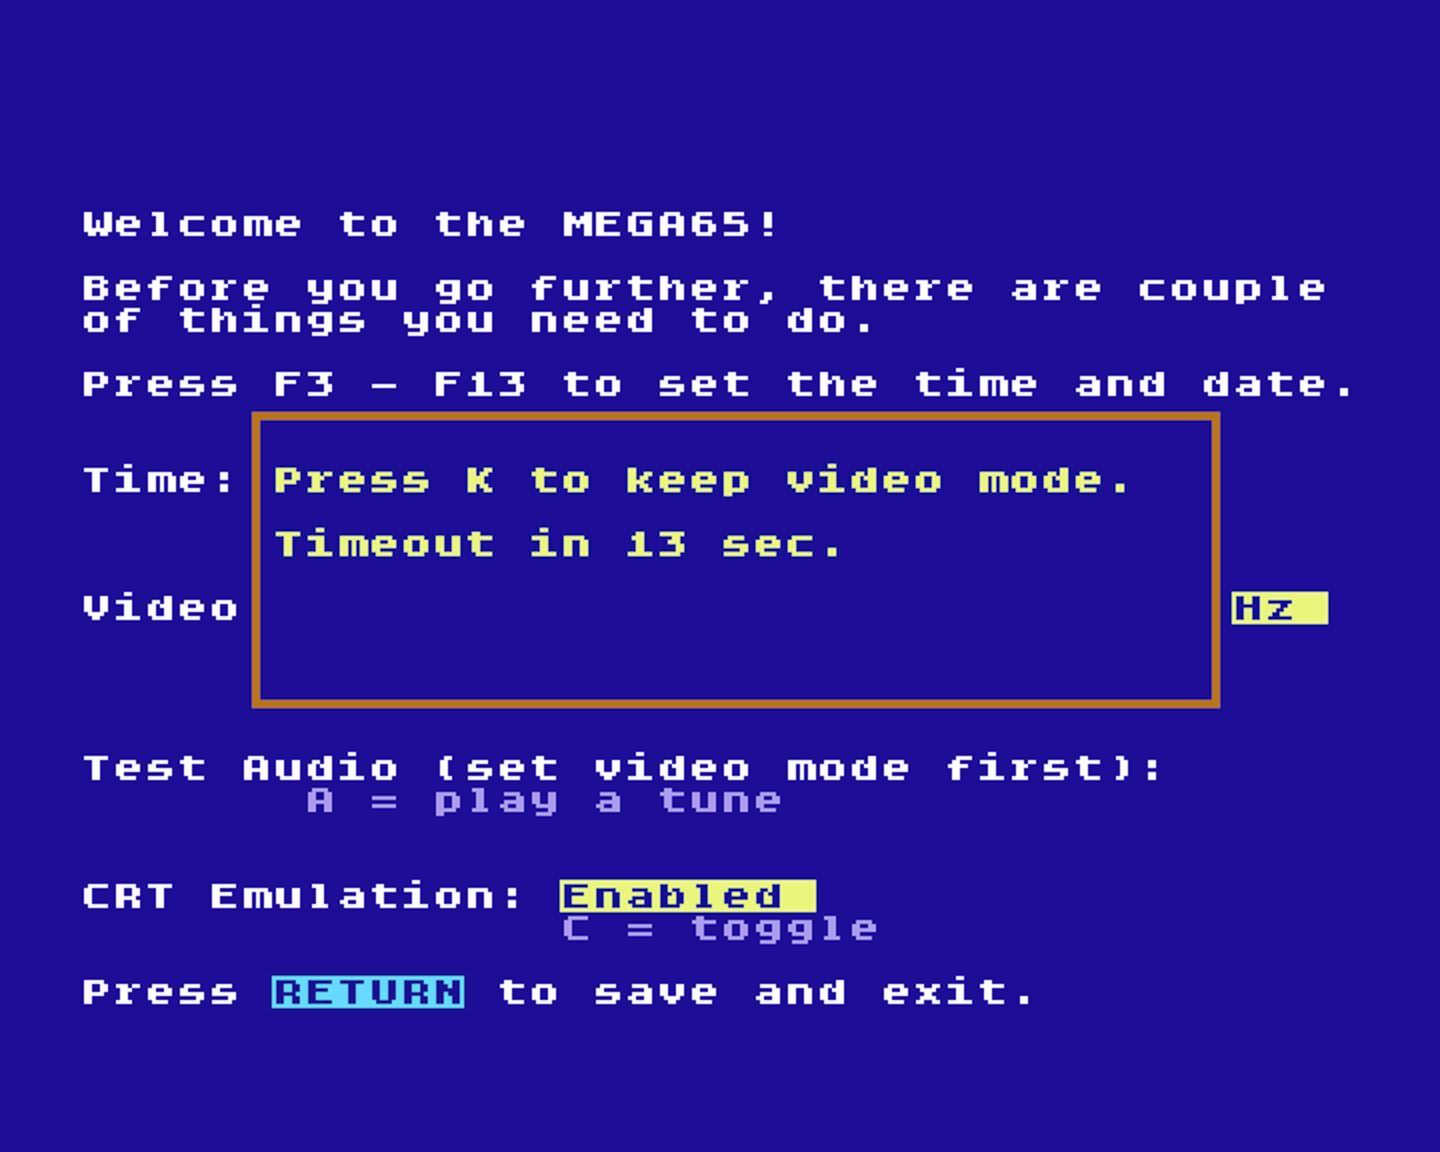
\includegraphics[trim= 20mm 20mm 10mm 25mm,clip,width=0.7\linewidth]{images/img011_final_boot_04.png}
\end{center}

Press \specialkey{RETURN} to complete the configuration:

\begin{center}
  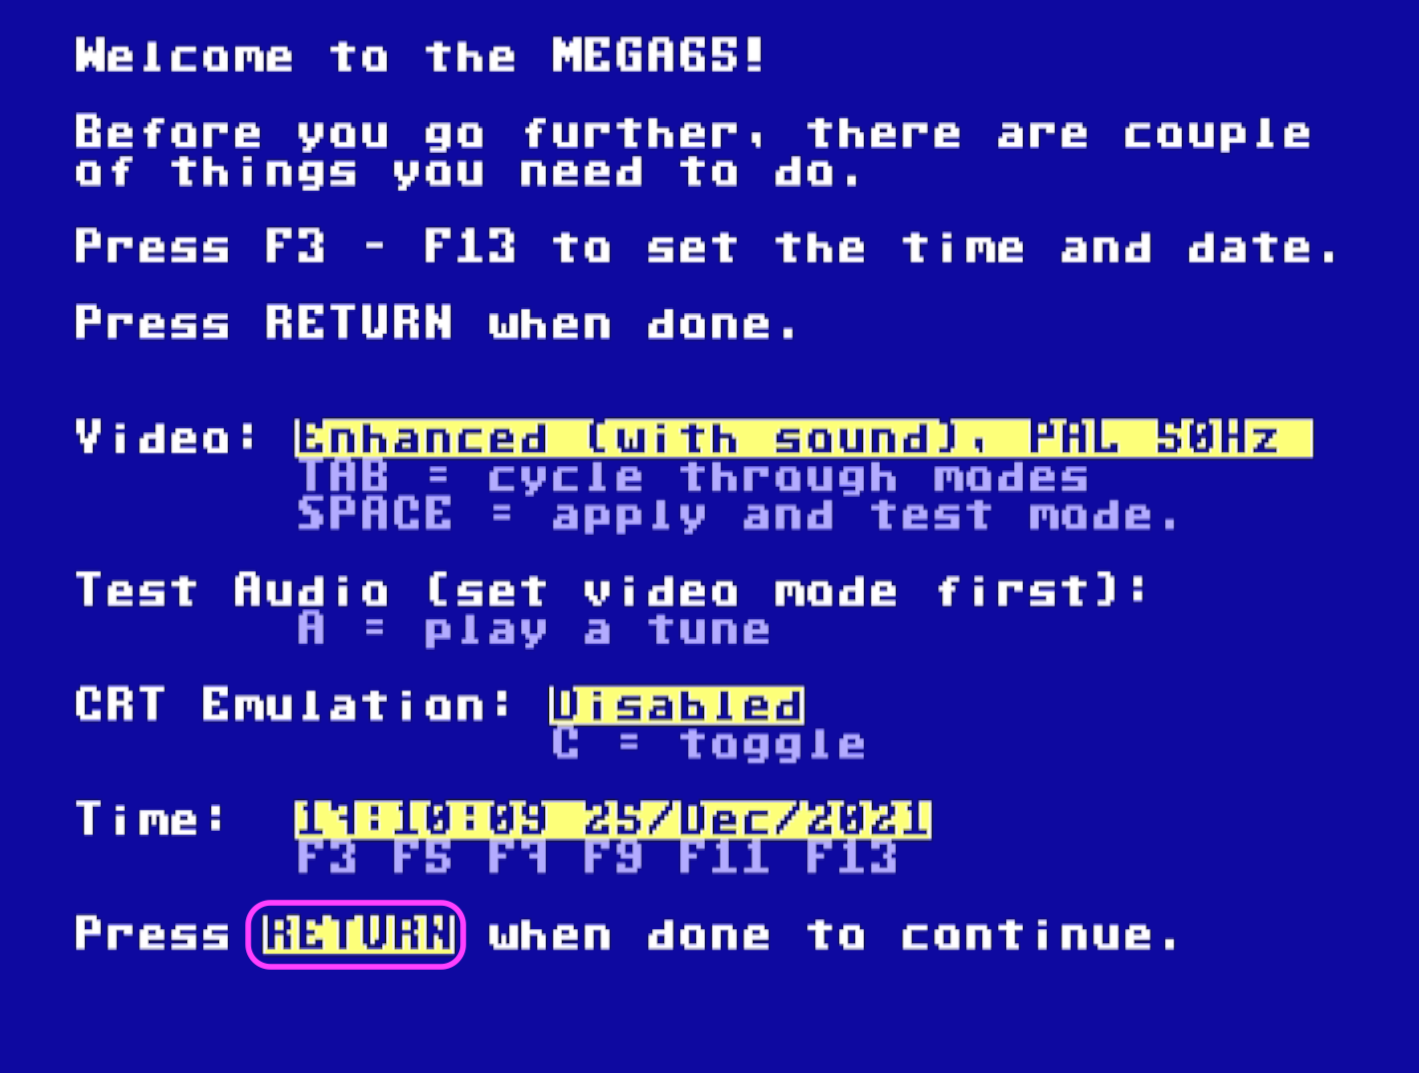
\includegraphics[trim= 6mm 6mm 6mm 6mm,clip,width=0.7\linewidth]{images/img011_final_boot_05.png}
\end{center}

\ifdefined\printmanual
\else
\textcolor{red}{\underline{Note for Nexys4 board users}: \\
\\
  At this very specific step, the board is supposed to reboot and display the main MEGA65 screen. If the board does not reboot and the screen remains black, then switch power to the board off then on again.}
\fi

After the MEGA65 reboots you will be greeted with the main MEGA65 screen:

\begin{center}
  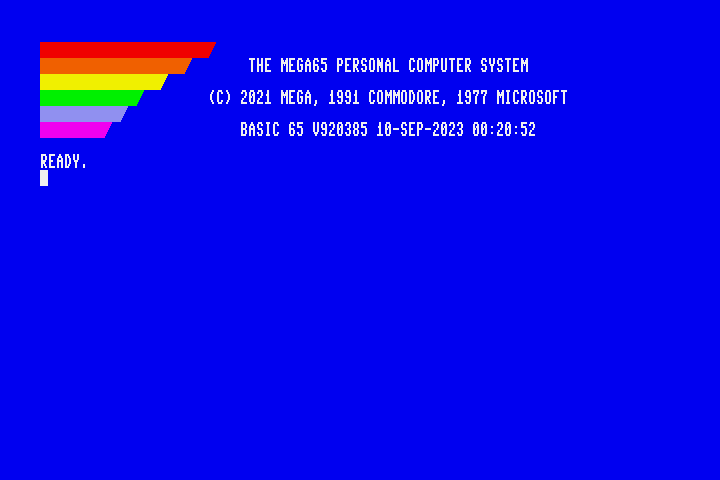
\includegraphics[trim=0 2cm 0 0,clip,width=0.7\linewidth]{images/img011_final_boot_06.png}
\end{center}

\section{Configuration Utility}
\label{sec:configuration-utility}

The configuration utility for the MEGA65 has a similar purpose to the BIOS on a PC, which is to allow you to control certain default behaviours of your MEGA65. However, rather than storing the configuration data in
battery-backed RAM, the MEGA65 stores this data on sector 1 of the SD card. If you switch SD cards, you will change the configuration data.

  To enter the configuration utility, switch the MEGA65 on while
  holding \specialkey{ALT} down.  This will show the utility menu,
  similar to the following:

\begin{center}
  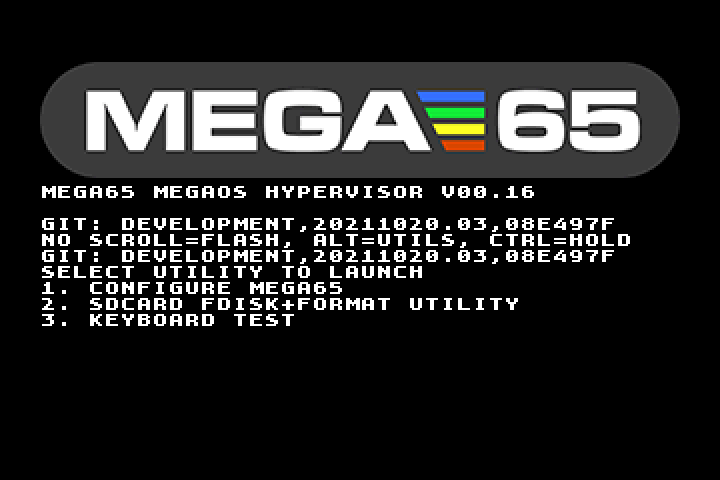
\includegraphics[width=0.7\linewidth]{images/ss-utilmenu.png}
\end{center}

%\begin{minipage}{\linewidth}
  Next, press the number corresponding to the \screentext{CONFIGURE MEGA65} item.  The MEGA65
  Configuration Utility will launch, showing a display similar to
  the following:

%  \vspace{5mm}
\begin{center}
  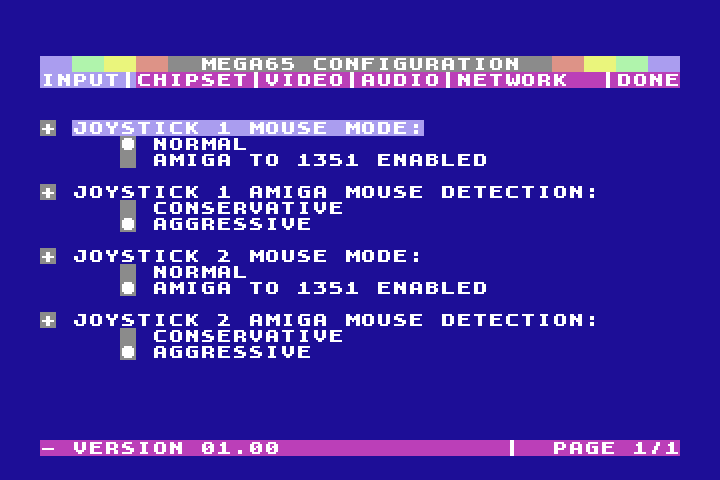
\includegraphics[width=0.7\linewidth]{images/ss-m65config-1.png}
\end{center}
%\end{minipage}

%\begin{minipage}{\linewidth}
  If your MEGA65's System Partition is corrupted, you may be
  prompted to press \megakey{F14} to correct this, (i.e., hold \specialkey{SHIFT} and press
  \megakey{F13}), with a display similar to the following:

%  \vspace{5mm}
\begin{center}
  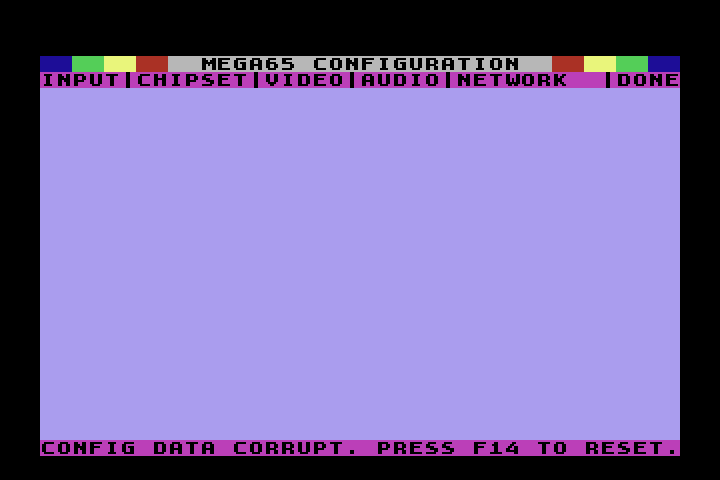
\includegraphics[width=0.7\linewidth]{images/ss-m65config-corrupt.png}
\end{center}
%\end{minipage}

To correct this error, press \megakey{F14}. Next, press \megakey{F7} to save the reset configuration, otherwise the reset data will not be saved to the MEGA65 System
Partition.

Once you have dismissed that display, or if your MEGA65 System Partition is not corrupt, you can begin exploring and adjusting various settings. The program can be controlled using the keyboard, or optionally, a 1351 or Amiga\texttrademark{} mouse.

You can advance screens by pressing \megakey{F1}, or use \megakey{F2} to navigate in the opposite direction. Use \megakey{$\leftarrow$} and \megakey{$\rightarrow$} to navigate between screens.

Use \megakey{$\uparrow$} and \megakey{$\downarrow$} to select an item.

Press \specialkey{RETURN} or \megakey{SPACE} to toggle a setting, or to change a text or numeric value. The black circle next to an option indicates the current selection.

  When you have finished, press \megakey{F7} to see the
  options for saving the changes. This will give you four options:

\begin{center}
  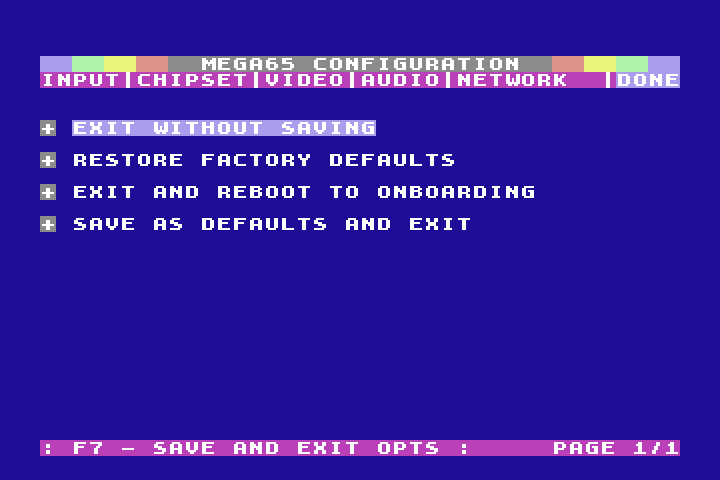
\includegraphics[width=0.7\linewidth]{images/ss-m65config-save.png}
\end{center}

\begin{itemize}
  \item \screentext {EXIT WITHOUT SAVING} abandons any changes made in the MEGA65 Configure utility and exits.
  \item \screentext {APPLY AND TEST SETTINGS NOW} uses the current settings immediately but does not exit. This is helpful to test compatibility of your TV or monitor with PAL or NTSC video modes. If you still see your display after applying a change, it is safe to save those settings.
  \item \screentext {RESTORE FACTORY DEFAULTS} resets the MEGA65 configuration settings to the factory defaults. It will randomly select a new MAC address for models that include an internal Ethernet adaptor. If you wish to commit these changes, you must still save them.
  \item \screentext {SAVE AS DEFAULT AND EXIT} commits changes made to the SD card. These changes will be used when the MEGA65 is switched on.
\end{itemize}

\subsection{Input Devices}

\begin{center}
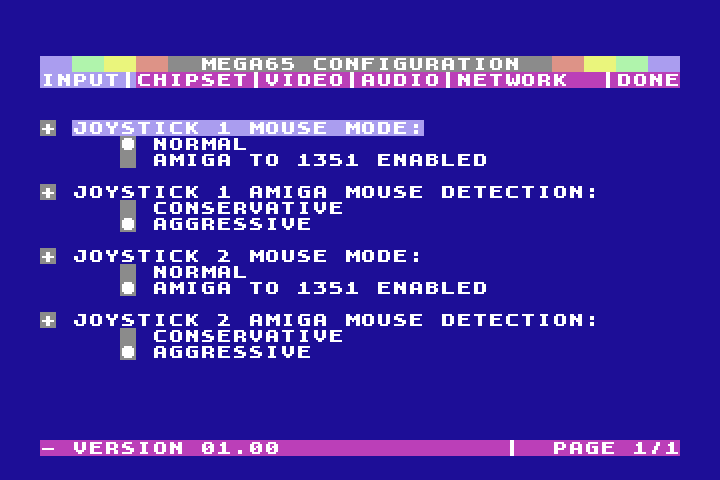
\includegraphics[width=0.7\linewidth]{images/ss-m65config-1.png}
\end{center}

\begin{itemize}
  \item \screentext{JOYSTICK 1 AMIGA MOUSE MODE} allows either \screentext{NORMAL} operation,
  where software will see it as an Amiga mouse or \screentext{1351 EMULATION} mode, where the MEGA65 translates the Amiga mouse's movements into 1351 compatible signals. This allows you to use an Amiga mouse with existing C64/C65 software that expects a 1351 mouse.
  \item \screentext{JOYSTICK 1 AMIGA MOUSE DETECTION} can be set to \screentext{CONSERVATIVE} or \screentext{AGGRESSIVE}. If you use an Amiga mouse and it fails to move smoothly in all directions, you may set it to \screentext{AGGRESSIVE}. Conversely, if you regularly use joysticks in the port, and have difficulties with the joystick input misbehaving, you might want to use the \screentext{CONSERVATIVE} option.
  \item \screentext{JOYSTICK 2 AMIGA MOUSE MODE} is identical to the first option, but for the second controller port. This allows you to have different settings for each port.
  \item \screentext{JOYSTICK 2 AMIGA MOUSE DETECTION} similarly provides the ability to separately control the Amiga mouse detection algorithm for the second controller port.
\end{itemize}


\subsection{Chipset}
\label{configuring-chipset}
\begin{center}
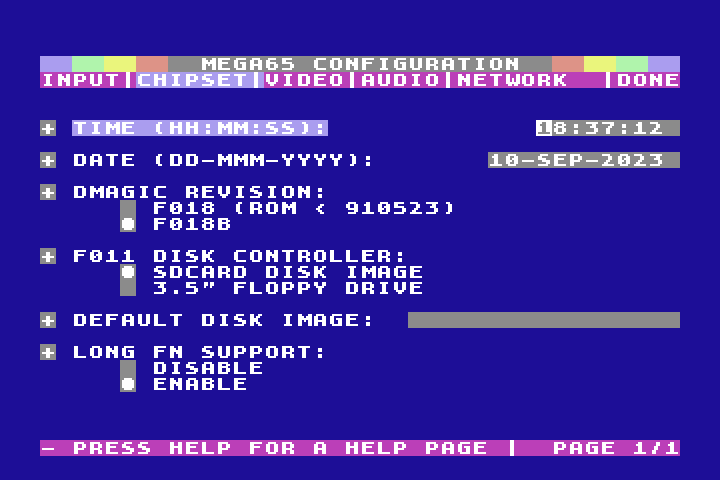
\includegraphics[width=0.7\linewidth]{images/ss-m65config-2.png}
\end{center}

\begin{itemize}
  \item \screentext{REAL-TIME CLOCK} allows setting the MEGA65's Real-Time
    Clock for those models that include one.  To set the clock or
    calendar, simply edit the field and press \specialkey{RETURN}.
    The display does not change while viewing this page, but if
    you use \megakey{$\leftarrow$} and \megakey{$\rightarrow$} to select another page and
    return to this page, the values will update if a Real-Time Clock
    is fitted and functioning.
  \item \screentext{DMAGIC REVISION} allows selecting the default mode of
    operation for the C65 DMAgic DMA controller.  This option is only
    required for ROMs not detected by the MEGA65's HYPPO Hypervisor.
    If you see screen corruption in BASIC,
    try toggling this option.
  \item \screentext{F011 DISK CONTROLLER}
    \index{Disk Drives!D81 Images}
    This option allows you to select whether the internal 3.5'' floppy
    drive functions using real diskettes, or whether it simply makes
    noises to add atmosphere when using D81 disk images from the SD
    card.  This merely sets the default option, and you can change
    this setting, or select a different disk image for use as either
    or both of the C65 3.5'' DOS based drives.
  \item \screentext{DEFAULT DISK IMAGE} allows you to choose the D81 disk image
    used with the internal drive, if the \screentext{F011 DISK CONTROLLER}
    option above is set to \screentext{USES SDCARD DISK IMAGE}. You can read more about
    D81 disk images on page \pageref{sec:d81-images}.
  \item \screentext{LONG FN SUPPORT} is a feature that is still under development
    at time of writing, and we suggest leaving it disabled for now until the feature
    matures in future bitstreams. Its aim is to provide long filename support for the
    SD card.
\end{itemize}

\subsection{Video}

\begin{center}
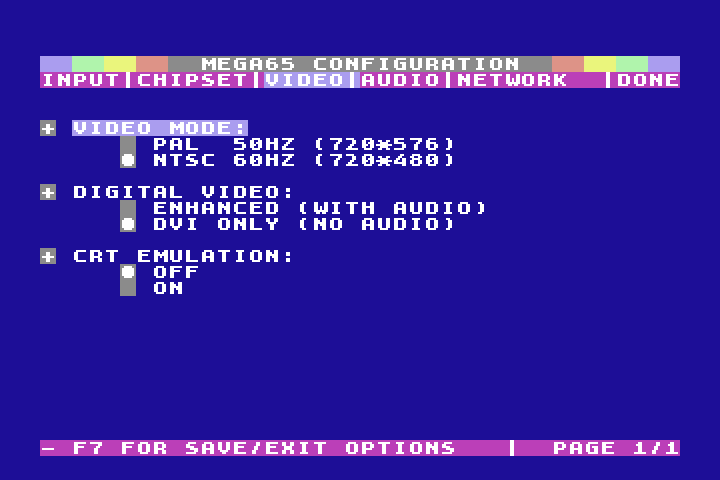
\includegraphics[width=0.7\linewidth]{images/ss-m65config-3.png}
\end{center}
\index{Display!Setting PAL/NTSC}
\begin{itemize}
  \item \screentext{VIDEO MODE} selects whether the MEGA65 starts in PAL or NTSC.    The MEGA65 supports true 480p NTSC and 576p PAL double-scan modes, with exact 60Hz / 50Hz frame-rates. This setting sets the default value, and the system can be switched between PAL and NTSC via the Freeze Menu, or under software control by MEGA65-enabled programs.
  \item \screentext{DIGITAL VIDEO} allows for selection between either \screentext{ENHANCED} video output containing audio, or \screentext{DVI ONLY} video output with no audio.
  \item \screentext{CRT EMULATION} selects whether CRT scanline emulation should be applied to the video output or not.
\end{itemize}

\subsection{Audio}

\begin{center}
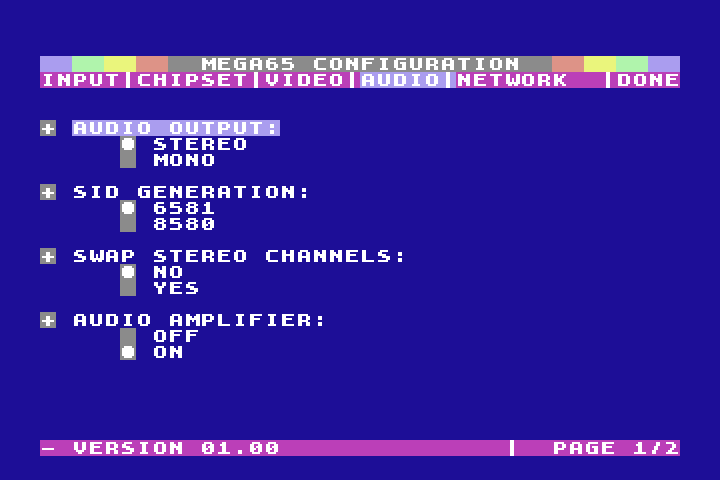
\includegraphics[width=0.7\linewidth]{images/ss-m65config-4.png}
\end{center}

\begin{itemize}
  \item \screentext{AUDIO OUTPUT} selects whether the SIDs and digital audio channels are combined to provide a monaural signal or whether the left and right tagged audio sources are separated to provide a stereo signal. This setting can be changed in the Audio Mixer of the Freeze Menu, or under the control of MEGA65-enabled software.
  \item \screentext{SWAP STEREO CHANNELS} allows switching the left and right-hand sides of the stereo audio output. This is useful for software that expects left and right SIDs to be at swapped addresses compared with the MEGA65 defaults.
  \item \screentext{DAC ALGORITHM} allows selecting between two different digital to analog conversion algorithms. Both options sound good and the selection is a personal preference.
  \item \screentext{AUDIO AMPLIFIER} allows enabling or disabling the audio amplifier contained in some models of the MEGA65. This option works for audio outputs, e.g., internal speaker or loud speaker.
\end{itemize}

\subsection{Network}

\begin{center}
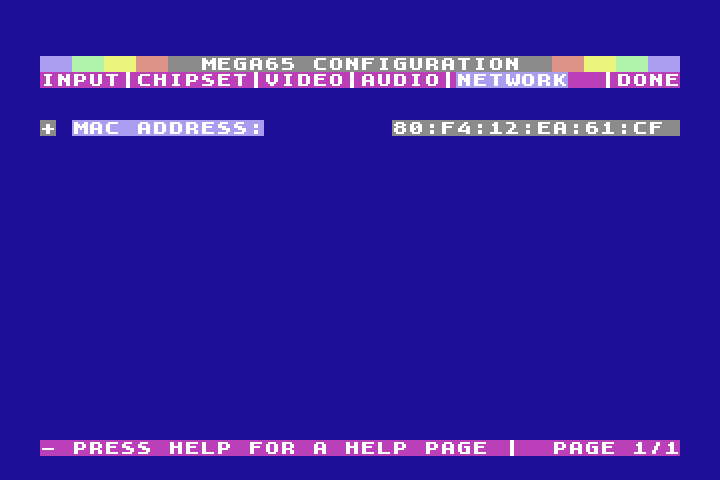
\includegraphics[width=0.7\linewidth]{images/ss-m65config-5.png}
\end{center}

\begin{itemize}
  \item \screentext{MAC ADDRESS} allows you to set the default MAC address of your MEGA65. This can be changed at run-time by MEGA65-enabled software.
\end{itemize}

% 2021-03-17 edits by SBC

\chapter {C64, C65 and MEGA65 Modes}
\label{cha:modes}

The MEGA65, like the C65 and the C128, has multiple operating modes.
However, there are important differences between the MEGA65 and both
of these earlier computers.

By default, the {\tt MEGA65.ROM} file boots to MEGA65-mode
(including BASIC 65), and
provides a method to switch to C64-mode via the \screentext{GO 64} command.
However, it is also possible to use an original C65 ROM (version {\tt 91XXXX.BIN})
renamed to {\tt MEGA65.ROM}, making the MEGA65 start in C65-mode
with BASIC 10. This also provides the same functionality to switch to C64-mode.

Therefore, dependent on your boot ROM choice, you have:

\begin{center}
\begin{tabular}{|l|l|l|l|}
 \hline
  {\textbf{Boot Mode}} & {\textbf{ROM version}} & {\textbf{BASIC}} & {\textbf{C64-mode}} \\
 \hline
   MEGA65    & \screentext{92XXXX}      & BASIC 65 & \screentext{GO 64} \\
   C65       & \screentext{91XXXX}      & BASIC 10 & \screentext{GO 64} \\
 \hline
\end{tabular}
\end{center}
For readers familiar with the C128,
the most important difference is that all of the MEGA65's new features
can be accessed from every mode, and that you can even switch back and forth
between the different modes. It's also possible to create hybrid modes that combine different
features from the different modes -- all you need is the {\bf MAP} instruction and the KEY register address,
which is {\bf 53295} (\$D02F).

This chapter explains the different modes, the {\bf MAP} instruction, and
the KEY register, which allows you to change the mode of operation of the MEGA65.
This chapter also explains how to use BASIC commands to switch from one mode to another.

\phantomsection
\section{Switching Modes from BASIC}

The MEGA65 is used in either C64-mode (running BASIC 2), C65-mode (running BASIC 10) for ROM versions {\tt 91XXXX},
or MEGA65-mode (running BASIC 65) for ROM versions {\tt 92XXXX}.

However, various MEGA65 features can be accessed from all modes, and all MEGA65 features are available
to programs written in assembly language / machine code.
\ifdefined\printmanual
For more information on how to write such programs, refer to the {\bf MEGA65 Book}.
\else
More information on how to write such programs can be found in the various appendices.
\fi

\subsection{From MEGA65/C65 to C64-mode}

To switch from MEGA65/C65 to C64-mode, use the familiar \screentext{GO 64} command, which is identical to switching to C64
mode on a C128:
\index{BASIC 65 Examples!GO64}
\begin{tcolorbox}[colback=black,coltext=white]
\verbatimfont{\codefont}
\begin{verbatim}
GO 64
ARE YOU SURE? Y
\end{verbatim}
\end{tcolorbox}

Note that any programs in memory will be lost in the process of switching modes. This is the same as the C128.
\index{Keyboard!MEGA Key}
Alternatively, you can hold \megasymbolkey down while pressing the reset button or switching the MEGA65 on. Again,
this is the same as the C128.

\subsection{From C64 to MEGA65/C65-mode}

To switch from C64 to MEGA65/C65-mode, use the following command. {\bf Note that this command does not ask you for
confirmation}!

\begin{tcolorbox}[colback=black,coltext=white]
\verbatimfont{\codefont}
\begin{verbatim}
SYS 58552
\end{verbatim}
\end{tcolorbox}

Alternatively, you can switch back to MEGA65/C65-mode by pressing the reset
button on the left-hand side of the MEGA65, or by switching the
MEGA65 off and on again.

Another option is to press and hold \widekey{RESTORE} for between half to one second, and then press \megakey {F5}
from the Freeze Menu.  This simulates pressing the reset button.

Note that any programs in memory will be lost in the process of switching modes. This is the same as the C128.

\subsection{Entering Machine Code Monitor Mode}

The Machine Code Monitor can be entered by typing either the {\bf MONITOR}
command from BASIC 65/10, or by holding \specialkey{RUN STOP}
down, and then pressing the reset button on the left-hand side of the
MEGA65.

\phantomsection
\section{The KEY Register}

The MEGA65 has a VIC-IV video controller chip instead of the C64's VIC-II or
the C65's VIC-III.  Just as the VIC-III has extra registers compared to the
VIC-II, the VIC-IV has even more registers.  If these were visible all the time,
software that was made for the C64 and VIC-II may inadvertently use these
new registers, resulting in unexpected behaviour.  Therefore, the
creators of the C65 created a way to hide the extra VIC-III registers from old
C64 programs. Enabling and disabling (or hiding and un-hiding) the extra registers is done via the KEY register. For more information
about which registers are disabled and enabled in each of the
VIC-II, VIC-III and VIC-IV I/O modes, refer to
\ifdefined\printmanual
 the {\bf MEGA65 Book}.
\else
 \bookvref{sec:iopersonalities}.
\fi

% iopersonalities results in ?? (??) when building on my machine

The KEY register, located at address {\bf 53295}, is an unused register of the VIC-II, which you can {\bf POKE} to and
 {\bf PEEK} from, similar to other registers. But the KEY register has a special function: If
you write two certain values to it in quick succession, you can tell the VIC-IV
to stop hiding the VIC-III or VIC-IV registers from the rest of the MEGA65.

\subsection{Exposing Extra C65 Registers}

For example, to enable the VIC-III's new registers when in C64-mode, you must {\bf POKE} the values 165 and 150
into the KEY register. The easiest way to do this is to switch your MEGA65 off and on again, and type GO 64
and answer Y to enter C64-mode.

\underline{Note}: If you perform these POKEs while in C65-mode, the MEGA65 may not function correctly.

Once you are in C64-mode, try typing the following commands:
\index{BASIC 65 Examples!POKE}
\begin{tcolorbox}[colback=black,coltext=white]
\verbatimfont{\codefont}
\begin{verbatim}
POKE 53295,165: POKE 53295,150
\end{verbatim}
\end{tcolorbox}

When you enter these commands, the MEGA65 returns a \screentextwide{READY.} prompt, and seemingly nothing else has
happened.  This is expected, because the MEGA65 has only enabled the VIC-III's new registers (and some other
C65-mode features). The C64 BASIC and KERNAL will still function as normal, and it may appear
that nothing has changed... But things \textit{have} changed.

For example, you can do something that the C64 and its VIC-II can't do: smoothly change one colour to another.
The VIC-III has registers that allow you to change the red, green and blue components of the colours. Now that the VIC-III
registers are enabled, it's possible to change the colour of the background progressively from blue to purple, by increasing
the red component of the colour that is normally blue on the C64.  The red component value registers are at
53504 -- 53759 (\$D100 -- \$D1FF). Blue is colour 6, so a change to register 53510 (53504 + 6, or \$D106) is required.
An example BASIC listing that includes a {\bf FOR} loop to change the colour is:

\begin{tcolorbox}[colback=black,coltext=white]
\verbatimfont{\codefont}
\begin{verbatim}
FOR I = 0 TO 15 STEP 0.2 : POKE 53510,I : NEXT
\end{verbatim}
\end{tcolorbox}

Once the program has been entered, type {\bf RUN} on a new line. This will make the background of the screen fade from
blue to purple.  If you would like to make the effect progress faster, increase the 0.2 to a larger number such as 0.5. To
make it slower, change it to a smaller number such as 0.02. You can also change the red component by {\bf POKE}ing a
different number to 53504 – 53759 (\$D100 – \$D1FF), the green component at 53760 -- 54015 (\$D200 -- \$D2FF), or the
blue component at 54016 -- 54271 (\$D300 -- \$D3FF).  For example, to have
the border and text (since they are both normally ``light blue'') fade from blue to green, you can try:

\begin{tcolorbox}[colback=black,coltext=white]
\verbatimfont{\codefont}
\begin{verbatim}
POKE 53518,0 : FOR I = 0 TO 15 STEP 0.1 : POKE 53774,I : POKE 54030,15-I : NEXT
\end{verbatim}
\end{tcolorbox}

\subsection{Disabling the C65/MEGA65 Extra Registers}

You can also disable the VIC-III registers again by {\bf POKE}ing any number into the KEY register, e.g.:

\begin{tcolorbox}[colback=black,coltext=white]
\verbatimfont{\codefont}
\begin{verbatim}
POKE 53295,0
\end{verbatim}
\end{tcolorbox}

If you {\bf RUN} the examples above again, the colours won't change because
the registers are disabled. Instead, writing to those addresses changes some of the VIC-II's registers,
as on a C64 they appear several times over.  Fortunately for the above example, the registers used have no obvious
side-effects. This is because the modified registers in the examples above on a standard VIC-II are used to change the
sprite positions. Since there are no sprites on the screen, you won't see anything change.

\subsection{Enabling MEGA65 Extra Registers}

The MEGA65 has \textit{even more} registers than the C65.  To enable these in C64-mode, it's required to {\bf POKE} another
two values into the KEY register:

\begin{tcolorbox}[colback=black,coltext=white]
\verbatimfont{\codefont}
\begin{verbatim}
POKE 53295,71: POKE 53295,83
\end{verbatim}
\end{tcolorbox}

Again, you won't see any immediate difference, which is similar to when enabling the VIC-III registers.  However, now the
MEGA65 can access not only the VIC-II and VIC-III registers, but also the VIC-IV registers.  If you like,
you can try the examples from earlier in this chapter to see that the VIC-III registers are accessible again.
But now you can also do MEGA65 specific things. For example, if you wanted to move the start of the top border higher
on the screen, you can try something such as:

\begin{tcolorbox}[colback=black,coltext=white]
\verbatimfont{\codefont}
\begin{verbatim}
POKE 53320,60
\end{verbatim}
\end{tcolorbox}

Alternatively, you can have some fun and animate the screen borders, by having them move closer and further apart:

\begin{tcolorbox}[colback=black,coltext=white]
\verbatimfont{\codefont}
\begin{verbatim}
FOR I = 255 TO 0 STEP -1 : POKE 53320,I : POKE 53322, 255 - I : NEXT
\end{verbatim}
\end{tcolorbox}

The above example has the loop count backwards (from 255 to 0), so that your don't end up with only a
tiny sliver of the text visible. You can make it go forwards if you like. If you do get stuck with only a sliver
of the screen, you can press \specialkey{RUN STOP} and \widekey{RESTORE}. You might be wondering: Why does \specialkey{RUN STOP}
and \widekey{RESTORE} work when these are VIC-IV registers that the C64-mode BASIC and KERNAL
don't know about?  The reason is the VIC-IV has a feature called ``hot registers'',
where certain C64 and C65 registers cause some MEGA65 registers to be reset to the C64 or
C65-mode defaults. In this particular case, it is the KERNAL resetting the VIC-II screen using
53265 (\$D011), which adjusts the vertical border size in C64/C65-mode, and is thus a ``hot register''
for the MEGA65's vertical border position registers.

See if you can make the screen shake around instead by changing the TEXTXPOS and TEXTYPOS registers of
the VIC-IV.  You can find out the {\bf POKE} codes for those, and lots of other interesting new registers
by looking through
\ifdefined\printmanual
 the {\bf MEGA65 Book}.
\else
 \bookvref{cha:viciv}.
\fi


\subsection{Traps to Look Out For}

In all modes, the DOS for the internal 3.5'' disk drive (including when you use D81 disk images from
an SD card) resets the KEY register to VIC-II mode whenever it is accessed. This means if you perform actions
such as check the drive status, or {\bf LOAD} or {\bf SAVE} a file, the KEY register will be reset, and only the VIC-II registers
will be enabled. You can of course enable the C65 or MEGA65 registers by {\bf POKE}ing the correct values
to the KEY register again.

\phantomsection
\section{Accessing Memory from BASIC 65}

BASIC 65 contains powerful memory banking and Direct Memory Access (DMA) commands that can be used to read,
fill, copy, and write areas of memory beyond the C65's 128KB of RAM.  The MEGA65 has 384KB of main memory, split into 6
banks of 64KB each. They are:
\begin{itemize}
 \item BANK 0 and BANK 1 - acts as the C65's normal 128KB RAM.
 \item BANK 2 and BANK 3 - normally write-protected, and contains the C65's ROM image.
 \item BANK 4 and BANK 5 - used for all graphic routines in BASIC 65 for high resolution bitplane graphics.
       BASIC 10 doesn't use banks 4 and 5.
\end{itemize}
\index{BASIC 65 Examples!BANK}
\index{BASIC 65 Examples!PEEK}
\index{BASIC 65 Examples!POKE}
Using the {\bf BANK}, {\bf PEEK} and {\bf POKE} commands, this region of memory can be easily accessed, for example:

\begin{tcolorbox}[colback=black,coltext=white]
\verbatimfont{\codefont}
\begin{verbatim}
BANK 4: POKE0,123: REM PUT 123 IN LOCATION $40000
BANK 4: PRINT PEEK(0): REM SHOW CONTENTS OF LOCATION $40000
\end{verbatim}
\end{tcolorbox}

Or, by using the {\bf DMA} command, you can copy the current contents of the screen and colour RAM into BANK 4 with:
\index{BASIC 65 Examples!DMA}
\begin{tcolorbox}[colback=black,coltext=white]
\verbatimfont{\codefont}
\begin{verbatim}
DMA 0, 2000, 2048, 0, 0, 4 : REM SCREEN TEXT TO BANK 4
DMA 0, 2000, DEC("F800"), 1, 2000, 4 : REM COPY COLOUR RAM TO BANK 4
\end{verbatim}
\end{tcolorbox}

You can then put something else on the screen, and copy it back with:

\begin{tcolorbox}[colback=black,coltext=white]
\verbatimfont{\codefont}
\begin{verbatim}
DMA 0, 2000, 0, 4, 2048, 0 : REM SCREEN TEXT FROM BANK 4
DMA 0, 2000, 2000, 4, DEC("F800"), 1 : REM COPY COLOUR RAM FROM BANK 4
\end{verbatim}
\end{tcolorbox}

\index{BASIC 65 Examples!MAP}
\phantomsection
\section{The MAP Instruction}

The above methods can be used from BASIC. In contrast, the {\bf MAP} instruction is an assembly
language instruction that can be used to rearrange the memory that the MEGA65 uses.
It is used by the C65 ROM and BASIC 65 to manage what memory it can use at any particular
point in time.  For further explanation of the {\bf MAP} instruction,
refer to the relevant section of
\ifdefined\printmanual
 the {\bf MEGA65 Book}.
\else
 \bookvref{sec:map-instruction}.
\fi




\chapter{Upgrading the MEGA65}

\section{How a MEGA65 Can Be Upgraded}
\label{cha:cores}

The MEGA65 platform consists of three major components:

\begin{enumerate}
  \item The {\bf MEGA65 core},\index{Core} a description of the chipset to run on the FPGA
  \item The {\bf ROM},\index{ROM} code that defines the Commodore-style operating system (KERNAL) and BASIC
  \item {\bf System software} for features such as the Freezer menu\index{Freezer menu}
\end{enumerate}

You can upgrade these components as new releases are published. You can also replace one or more of these components individually. In the case of the core and ROM, you can even have multiple versions installed simultaneously and switch between them. For example, instead of the latest MEGA65 ROM, you can switch to the original Commodore 65 prototype ROM. Or, you could switch to another core that causes your MEGA65 hardware to behave like a different computer entirely, such as a Commodore 64 or a ZX Spectrum.

The ROM and system software are files that reside on the SD card, and upgrading them is as simple as replacing the files. To upgrade the core, you use a process to install a core file into the MEGA65's core flash memory. This chapter describes this process.

\subsection{What is a Core?}
\index{Core!definition}

The MEGA65 hardware architecture is based on a versatile chip called a ``Field Programmable Gate Array,'' or FPGA.\index{Field Programmable Gate Array (FPGA)} This is a special kind of computer chip that can be programmed to impersonate other chips. They do this by configuring a giant array of logic gates to reproduce circuits. FPGAs are not an emulation, but an electronic re-creation of other chips. FPGA code is sometimes referred to as {\em firmware,} a term you may recognize from modern computers and other devices.

Your MEGA65 was programmed at the factory to re-create a chipset designed by the MEGA65 team, based on the original Commodore 65. You can re-program the MEGA65 FPGA to upgrade to new versions of the MEGA65 chipset, or to replace the chipset with that of an entirely different computer!

Each possible chipset is known as a {\em core}. The MEGA65 can store up to eight cores, and you can switch between these cores by accessing a menu when you switch on the computer. You can also use this menu to load a new core from a file on the SD card, a process known as {\em flashing}.

Members of the MEGA65 community have made several useful and fun alternate cores for the FPGA hardware. \href{https://github.com/MJoergen/C64MEGA65}{{\em C64 for MEGA65}} by MJoergen and sy2002 re-creates the original Commodore 64 computer with a high degree of accuracy, perfect for running Commodore 64 games, demos, and applications. Other cores re-create the ZX Spectrum, the Game Boy, and even the original Galaga arcade machine hardware. The MEGA65 team believes that the FPGA is powerful enough to re-create nearly all 8-bit home computers, and likely some 16-bit computers and consoles such as the Commodore Amiga. The MEGA65 hardware design, board layout, FPGA core, and other information are all available for free under various open-source licenses, so anyone is free to create other cores for the MEGA65 hardware.

\section{Determining the Versions of Things}
\label{sec:versions}

All components of the MEGA65 platform have a version identifier. The MEGA65 can display the version identifiers for all of its components using the MEGA65 Information utility.\index{MEGA65 Information Utility}

To open the MEGA65 Information utility:

\begin{enumerate}
  \item Switch on the MEGA65, and allow it to boot to BASIC.
  \item Open the Freezer:\index{Freezer menu} press and hold \widekey{RESTORE} for one second then release it.
  \item Press \specialkey{HELP}. The MEGA65 Information utility will open.
\end{enumerate}

\begin{center}
  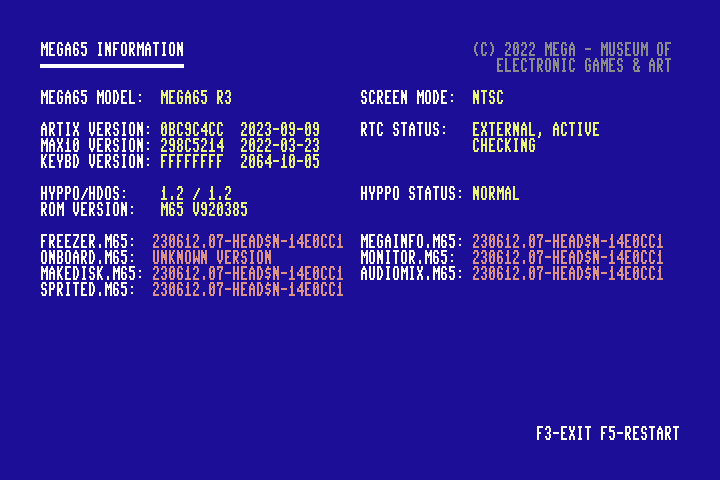
\includegraphics[width=0.7\linewidth]{images/megainfo.png}
\end{center}

Take note of these version identifiers:
\nopagebreak
\begin{center}
\setlength{\tabcolsep}{1mm}
\begin{tabularx}{\textwidth}{|X|p{7cm}|}
  \hline
  {\bf Label and Example} & {\bf Description} \\
  \hline
  MEGA65 Model\newline {\tt MEGA65 R5} & The revision of the hardware. You need to know this when downloading new core files. \\
  \hline
  Artix Version\index{Core!Version}\newline {\tt 93D55F08 2022-10-12} & The currently running MEGA65 core. This is a string of eight letters and numbers, and also a build date. \\
  \hline
  ROM Version\index{ROM!Version}\newline {\tt M65 V920377} & The currently running ROM. For MEGA65 ROMs, this is a sequential number, with larger numbers representing newer releases. \\
  \hline
  System files (.M65)\newline {\tt 221012.18-MASTER-5BBFDA9} & Each of the system software files has its own version identifier. Typically, you do not need to know these: you will upgrade these along with each core. The identifier is similar to the core version, but does not always match the currently running core. \\
  \hline
\end{tabularx}
\end{center}

Press \specialkey{F3} to exit to the Freezer, then \specialkey{F3} again to exit to BASIC.

Each core has a separate version for each hardware revision. As of the year 2023, the production models of the MEGA65 have used two different main board revisions, known as ``R3'' (more specifically ``R3A'') and ``R5.''\footnote{The MEGA65 ``DevKit'' model sold in the year 2020 is revision ``R3.'' It is also possible to run the MEGA65 core on certain FPGA development boards, with a separate version of the core file for each.}\index{Hardware revisions}

The MEGA65 core is available for all hardware revisions. If you are installing an alternate core and it is not available for your hardware revision, contact the author of the core.

\section{Obtaining the Latest Files}

You can download the latest MEGA65 core, ROM, and system software from the MEGA65 Filehost website.\index{Filehost website} Due to distribution restrictions for the Commodore 65 ROM code, some files require a Filehost account registered to a MEGA65 owner to access. All owners of the MEGA65 have a license to all versions of this ROM code.\footnote{There is a procedure for non-owners to get the latest MEGA65 ROM, such as to use with the \href{https://github.lgb.hu/xemu/}{Xemu MEGA65 emulator}. This involves downloading \href{https://www.c64forever.com/}{C64 Forever Free Express Edition} from Cloanto, extracting the original Commodore 65 prototype ROM file, then using a tool to apply a patch that you can download from Filehost. The full process is described in the following article: \url{https://files.mega65.org?ar=145591dd-deb6-4bd0-aa89-8e39cd021470}}

Visit the following URL in your web browser:

\url{https://files.mega65.org}

\begin{center}
  \fbox{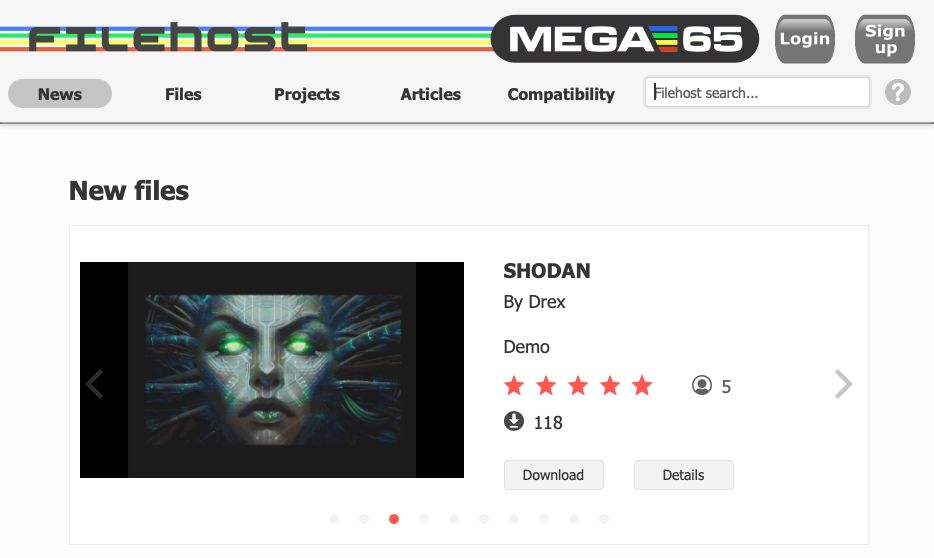
\includegraphics[width=0.7\linewidth]{images/filehost_notsignedin.png}}
\end{center}

To register a Filehost account with your owner code:

\begin{enumerate}
  \item Visit \href{https://files.mega65.org}{the Filehost website}. Click ``Sign Up.'' Follow the prompts to create an account.
  \item Locate your owner code.\index{Owner Code} This is a code printed on a piece of paper that was included with your MEGA65 (possibly inserted into this manual). It looks something like this: {\tt 123-ABC-456}
  \item Click the user icon in the upper-right corner of the Filehost screen. In the pop-up menu, select ``Redeem Code.'' Enter your owner code as prompted.
\end{enumerate}

\begin{center}
  \fbox{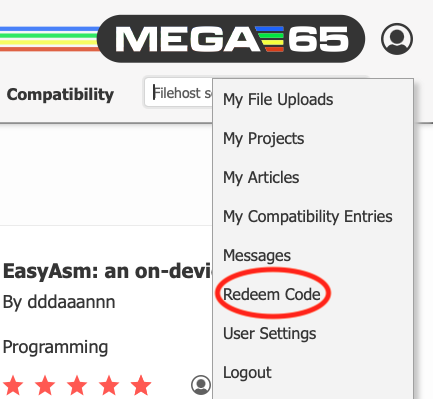
\includegraphics[width=0.4\linewidth]{images/filehost_redeemmenu.png}}
\end{center}

To download the latest release package:

\begin{enumerate}
  \item Click the ``Files'' tab of the Filehost website.
  \item In the search box on the left-hand side, type: ``release'' The list will update to show only files with that word in the title.
  \item Locate the entry named, ``MEGA65 Core Release Package (mega65r5) incl. ROM,'' where ``mega65r5'' matches your hardware revision. (To confirm your hardware revision, open the Freezer menu, then press \specialkey{Help}.)
  \item Click the entry. Confirm that this release package is for your hardware revision, then click ``Download'' to download the file.
\end{enumerate}

If you don't see an entry that says ``incl. ROM,'' check that you are signed in and that you have redeemed a valid owner code. Note that there is an entry for the Release Package that does not include the ROM that is visible to everyone. To ensure you are using a compatible set of files, get the package that says ``incl. ROM.''

\begin{center}
  \fbox{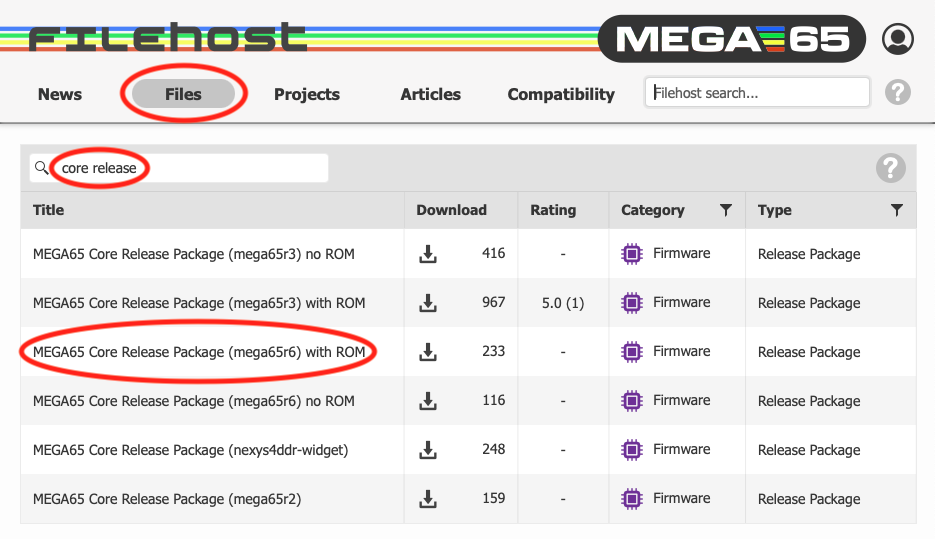
\includegraphics[width=0.7\linewidth]{images/filehost_release.png}}
\end{center}

Extract the downloaded {\tt .7z} archive. You should see a file whose name ends in {\tt .cor}, and a folder of {\tt sdcard-files} that includes one named {\tt MEGA65.ROM}.

\section{The Core Selection Menu}
\index{Core!Core Selection Menu}

The MEGA65 decides which core to load into the FPGA when it starts up. You can interrupt this process to select which core to load.\footnote{Technically, the MEGA65 starts the core in slot 0 to power the core selection menu. After you have made a selection or it chooses a default, it loads the selected core into the FPGA and continues the boot process.}

To open the core selection menu, switch off the computer, then hold the \specialkey{NO\\SCROLL} key and switch on the computer. The core selection menu appears, with the eight core slots numbered 0 through 7.

\begin{center}
  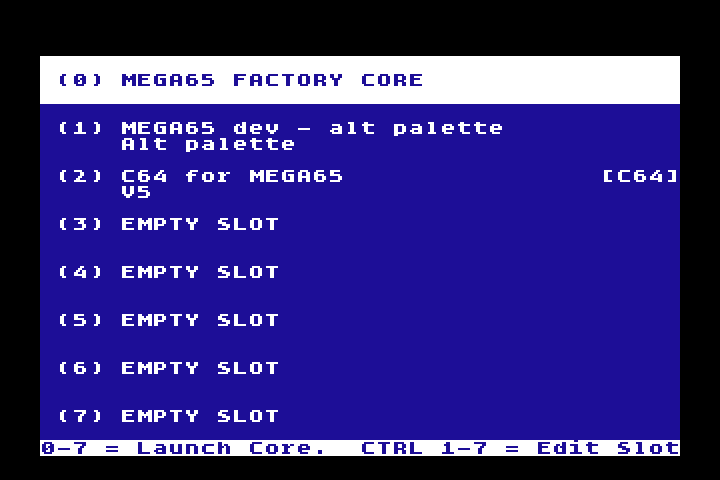
\includegraphics[width=0.7\linewidth]{images/ss-flashmenu.png}
\end{center}

You can select a core to boot using the cursor keys and \specialkey{RETURN}, or you can simply press the number key that corresponds to the slot. The boot process continues with the new core. The MEGA65 will keep running the new core until you physically power it off. (Pressing the reset button will not reset which core is being run.)

When you switch on the computer without opening the core selection menu, the MEGA65 looks for a core in slot 1. If there is a valid core in that slot, it uses it. Otherwise it tries slot 0.\footnote{You can change the default core slot from 1 to 2 by moving DIP switch \#4 to the ``on'' position. DIP switches are located inside the case, on the main board. For a diagram of the DIP switch locations, see \vref{cha:transferring-files}.}

Your computer comes with the MEGA65 core in slot 0 installed at the factory. It is recommended that you do not upgrade the factory-installed core under most circumstances. Instead, install new versions of the MEGA65 core in slot 1.

\section{Upgrading the MEGA65 Core, ROM, and System Files}
\index{Core!Upgrading}\index{ROM!Upgrading}

You can upgrade a core or install a new core from the core selection menu. This process reads the {\tt .cor} file from the SD card.

To upgrade the MEGA65 core, ROM, and system files:

\begin{enumerate}
  \item Remove the SD card (or microSD card) from the MEGA65, and connect it to your PC using an SD card reader.\footnote{As an alternative to moving the SD card to your PC, you can transfer files using an Ethernet connection. See chapter \vref{cha:transferring-files}.}
  \item Copy the {\tt .cor} file that you extracted from the {\tt .7z} archive to the SD card.
  \item On your PC, open the {\tt sdcard-files} folder from the {\tt .7z} archive, then copy those files to the SD card, replacing the existing files. Put them in the root of the SD card's file system, not a sub-folder.
  \item Eject the SD card from your PC's operating system, then move it back to the MEGA65.
  \item Open the core selection menu: Switch off the MEGA65, then hold \specialkey{NO\\SCROLL} while switching it back on.
  \item Hold \specialkey{CTRL} then press the number of the slot you want to upgrade. Follow the prompts. This process asks for a key press several times, and takes several minutes.
\end{enumerate}

When you start the update process, it prompts you to select the {\tt .cor} file on a screen that looks similar to this:

\begin{center}
  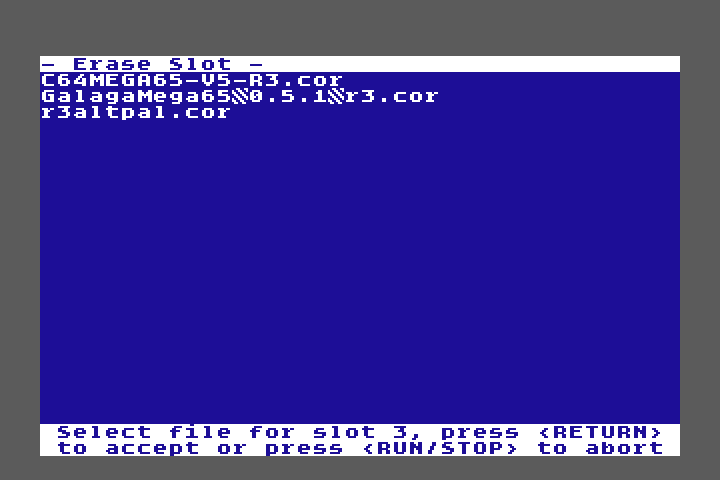
\includegraphics[width=0.7\linewidth]{images/ss-flashmenu-selectcore.png}
\end{center}

The process begins by checking that the core file matches your hardware revision. Press any key to continue.

\begin{center}
  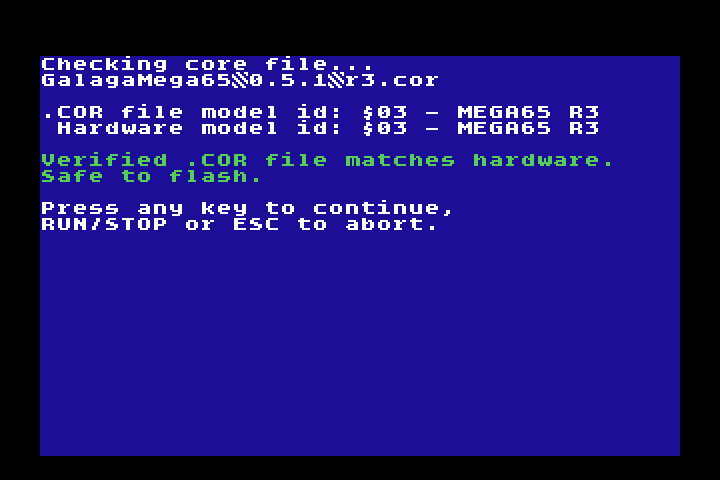
\includegraphics[width=0.7\linewidth]{images/ss-flashmenu-1-checking.png}
\end{center}

It then copies the file from the SD card to RAM, performing another check that the core file is complete.

\begin{center}
  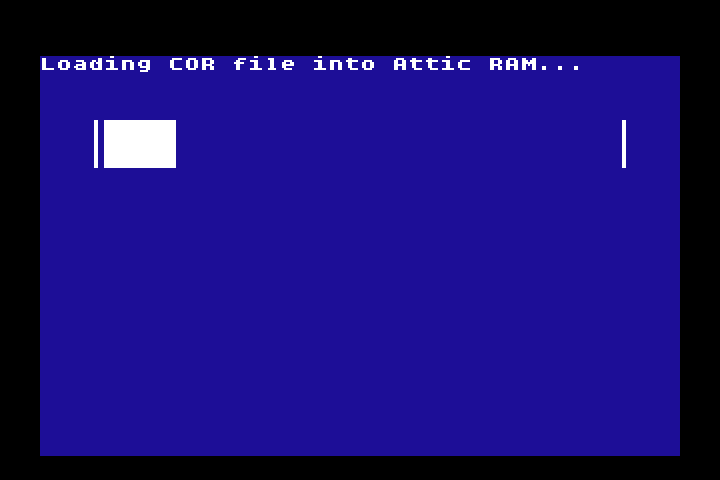
\includegraphics[width=0.7\linewidth]{images/ss-flashmenu-2-loading.png}
\end{center}

It presents the result of this check before proceeding. If the check is valid, you will see a message similar to the following. Press any key to continue.

\begin{center}
  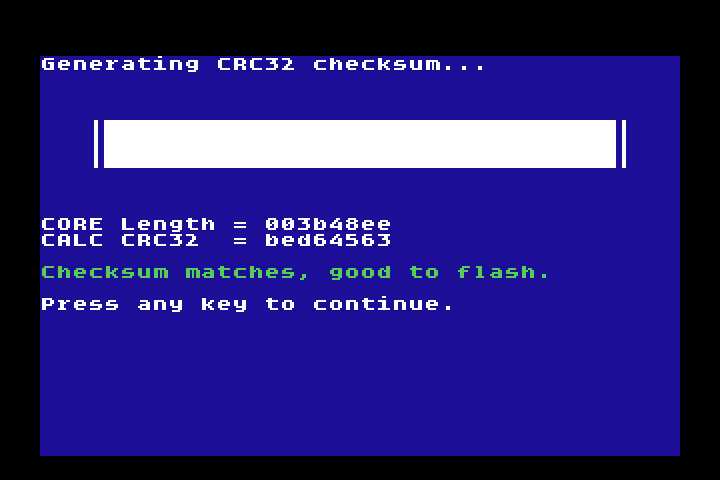
\includegraphics[width=0.7\linewidth]{images/ss-flashmenu-3-checksum-ok.png}
\end{center}

If the check is invalid, you will see the message, ``CHECKSUM MISMATCH.'' If you were not expecting this message, abort the process and confirm that you are using the correct file.\footnote{There are rare cases where a core may be valid but not have a correct checksum, such as if you are installing older versions of the core.}

Once you tell it to proceed, the MEGA65 begins programming the core data into flash memory. The border twinkles in coloured patterns during this process.

\underline{Note}: Do {\em not} switch off your computer or disconnect power until after this step is complete.

\begin{center}
  \fbox{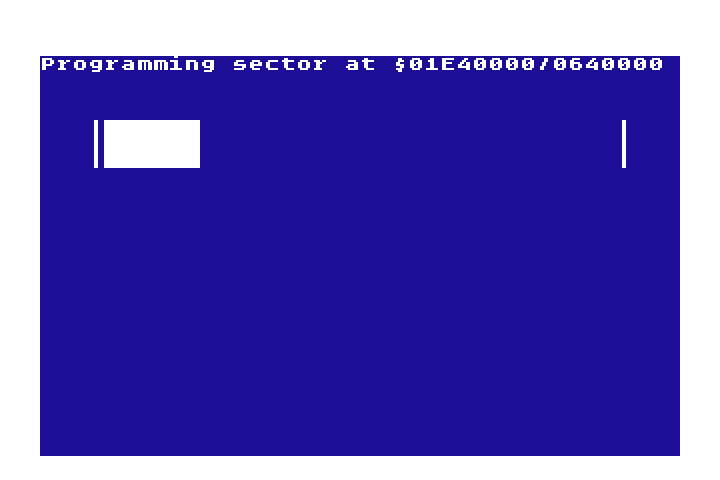
\includegraphics[width=0.7\linewidth]{images/ss-flashmenu-4-programming.png}}
\end{center}

When the process is complete, you will see a screen similar to the following.

\begin{center}
  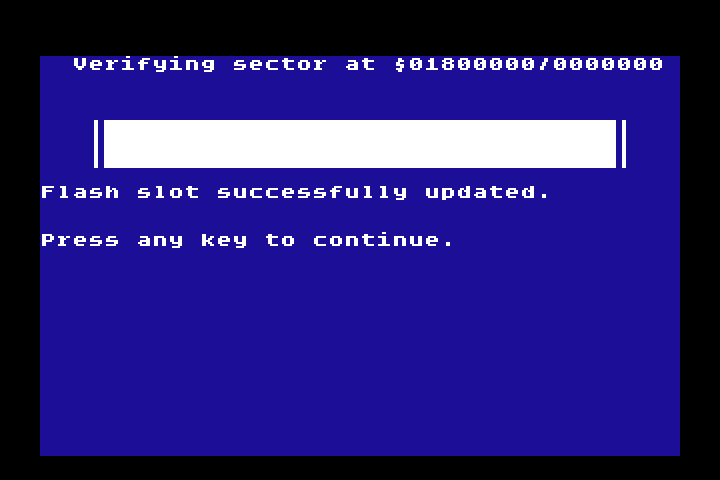
\includegraphics[width=0.7\linewidth]{images/ss-flashmenu-done.png}
\end{center}

It is now safe to switch off your computer. Press any key to return to the core selection menu, or switch the computer off then on again to start the default core.


\section{Installing Alternate Cores}

Installing an alternate core, such as the C64 core,\index{Core!C64 core} uses the same steps for flashing the core to a slot.

It is recommended to use slots 2 through 7 for alternate cores, and reserve slot 1 for the latest MEGA65 core. Of course, there is nothing stopping you from installing an alternate core in slot 1, so that the MEGA65 behaves as a different type of computer when you switch it on. You can always choose the MEGA65 core from the core selection menu.


% TODO: Document how to configure the boot core for cartridge types


\section{Upgrading the Factory Core in Slot 0}
\index{Core!Upgrading Slot 0}

It is possible to upgrade the factory-installed MEGA65 core in slot 0. You only need to do this in rare cases, such as if a newer version of the MEGA65 core includes changes or bug fixes for the start-up process. The process is elaborate, delicate, and could result in a MEGA65 that fails to start if something goes wrong. It is {\em strongly} recommended that you do not upgrade slot 0 unless the announcement for the release suggests that you do so. Most MEGA65 core upgrades are fully functional in slot 1, without needing to upgrade slot 0.

{\em Please read these instructions carefully before starting the procedure.}

\begin{enumerate}
  \item Prepare to use the {\em internal SD card only}. This may involve opening the case to make the SD card easier to access. Do {\em not} use the external microSD card slot for updating core slot 0.
  \item Using your PC, rename the core file that you wish to install to this exact filename: {\tt UPGRADE0.COR} (That's the word {\tt UPGRADE}, the number zero, and {\tt .COR}, using uppercase letters.)
  \item Install the latest MEGA65 core in slot 1, using the procedure described earlier. The core must be in the default non-zero slot to recover from any problems when updating slot 0. Boot this core to test that it works.
  \item Open the core selection menu. Press \megasymbolkey and the comma key to start the flash procedure for slot 0. (You will not be prompted for a filename.)
\end{enumerate}

\ifdefined\printmanual
\else
\underline{Note}: If you have a revision R3A MEGA65, have not previously upgraded slot 0, and \megasymbolkey and \megakey{,} does not start the procedure, you have an older slot 0 core that does not have this feature. You can work around this by restarting the core selection menu with slot 1. From the core selection menu, prepare to hold down \specialkey{NO\\SCROLL}, press the \megakey{1} key to boot into the core then immediately press and hold \specialkey{NO\\SCROLL}. The core selection menu re-opens using slot 1. Press \megasymbolkey and the comma key to complete the slot 0 upgrade.
\fi

If something goes wrong during the slot 0 flashing process, your MEGA65 may not start correctly. Before doing anything else, switch on your MEGA65, and wait a minute or so. It should notice that there is no valid core in slot 0, then proceed to start the core in slot 1. You can hold \specialkey{NO\\SCROLL} during this to open slot 1's core selection menu and restart the flashing process.

If the MEGA65 cannot boot any core after several minutes, it may be stuck. You may be able to recover using a device known as a ``JTAG interface'' that connects your PC to the MEGA65 main board. This allows you to inject a bitstream directly into the FPGA. The part is inexpensive but not always available. Contact the MEGA65 team on the Discord (\url{https://mega65.org/chat}) for assistance.


\section{Installing Alternate ROMs}

You can keep more than one version of the MEGA65 ROM on the SD card. When booting the MEGA65 core, you can select one of these ROMs by holding down a number key during boot.

To install alternate ROMs, copy them to the root of the SD card with a filename such as {\tt MEGA65x.ROM}, where {\tt x} is a number between 1 and 7. To boot the alternate ROM, hold the corresponding number key down while the MEGA65 core starts. If you do not hold down a number, it boots to {\tt MEGA65.ROM} by default.

There are several reasons you might want to keep alternate ROMs on your SD card:

\begin{itemize}
  \item You are helping to test a new beta release of the ROM, and do not wish to make the beta version your default ROM.
  \item You want to try the MEGA65 OpenROM, a project to create an all-new ROM released under an Open Source license without any original Commodore material.
  \item You want to try the original Commodore 65 prototype ROM. The MEGA65 core maintains backwards compatibility with the C65 ROM that was in progress by Commodore before they cancelled the project. It is buggy and incomplete, but is still an interesting historical artifact.
\end{itemize}

Several alternate ROMs came with your MEGA65 SD card, installed at the factory. Try rebooting your computer while holding down a number key to see what happens!


\section{Understanding The Core Booting Process}
\nopagebreak
This section summarises how the MEGA65 selects which core to start with when it is switched on. The process is shown in the following figure:
\nopagebreak
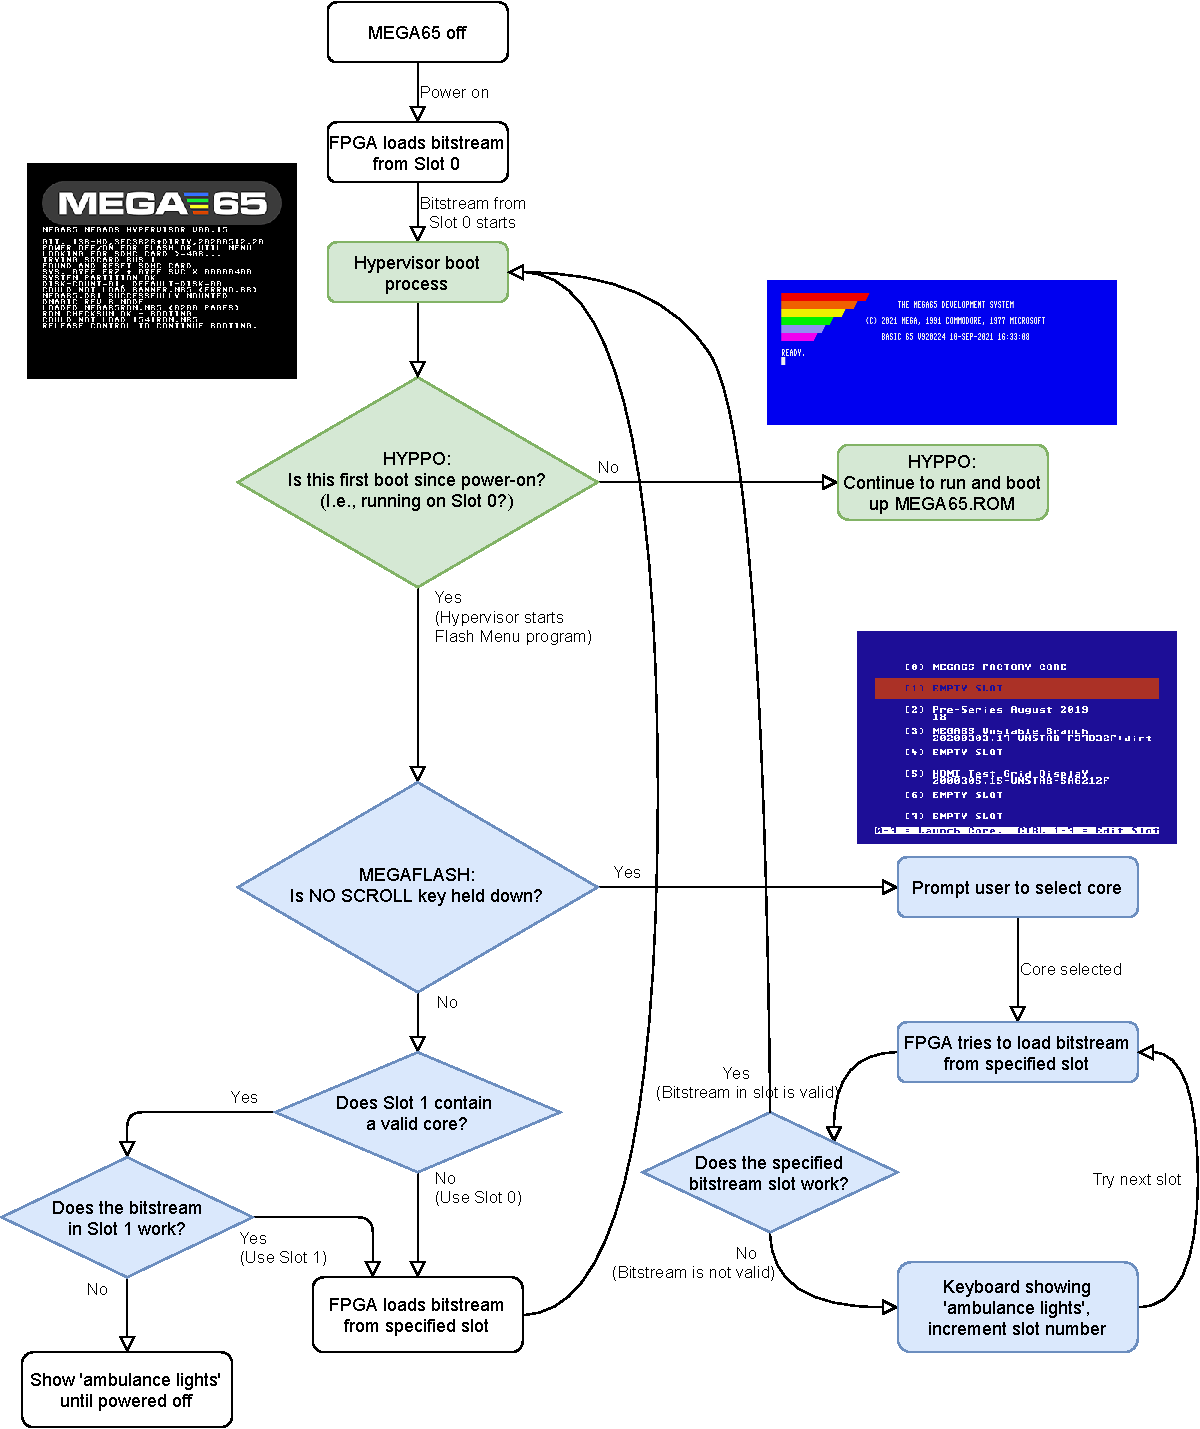
\includegraphics[width=\linewidth]{images/illustrations/flashmenu-flowchart.pdf}

The booting process is governed by two facilities:
\begin{itemize}
  \item The Hypervisor (also known as HYPPO), which operates at a level above the KERNAL. One of its responsibilities is to manage aspects of the boot process. For more details on the Hypervisor, refer to
\ifdefined\printmanual
the {\bf MEGA65 Book}.
\else
 \bookvref{sec:hypervisor-mode}.
\fi
    In the diagram, activities performed by the Hypervisor have been highlighted in green.
  \item The Core Selection Menu program (also known as ``MegaFlash''), which provides a list of available core slots to choose from. In the diagram, activities performed by MegaFlash have been highlighted in blue.
\end{itemize}

When the MEGA65 is switched on, it does the following:
\begin{itemize}
\item Loads the bitstream stored in slot 0 of flash memory. If that is the MEGA65 Factory Core, the MEGA65
  HYPPO Hypervisor starts.
\item If it is the first boot since power-on (which implies that you are running from slot 0), HYPPO starts the Flash Menu program (aka MegaFlash) -- but note that the Flash Menu in
      this mode may not show anything on the screen to indicate that it is running!
\item The Flash Menu then checks if \specialkey{NO\\SCROLL} is being held down.
\item If it is, the Flash Menu program shows its display, allowing you to select or re-flash a core.
\item If \specialkey{NO\\SCROLL} is {\em not} being held down, the Flash Menu program checks if Flash Slot 1 contains a valid
      core.
\item If it does, then the Flash Menu program attempts to load that core.
\item If it succeeds, then the system reconfigures itself for that core, after which the behaviour of the system is
      according to that core.
\item If it fails, the keyboard will go into ``ambulance mode'', showing flashing blue lights to indicate that some
      first-aid is required. Note that in ambulance mode the reset button has no effect: You must switch the
      MEGA65 off and on again.
\end{itemize}

If you have selected a different core in the Core Selection Menu, the process is similar, except that the ambulance lights will appear for only a limited time, as the FPGA will automatically search through the flash memory until it finds a valid core. If it gets to the end of the flash memory, it will start the MEGA65 Factory Core from slot 0 again.

\chapter{Floppy Disks, the Freezer, and D81 Images}
\label{cha:freezer}

\phantomsection

\section{Disk Drives}
\index{Disk Drives}
The MEGA65 is compatible with a wide range of floppy disk drives, and can be configured to use them in a variety
of different ways. It includes an internal 3.5" drive, which is compatible with double density and high density
3.5" disks. But did you know you can also use 5.25" disks? By connecting a compatible IEC drive to the rear
Floppy Disk Drive/IEC Connector, you can use your MEGA65 with two or more physical floppy drives simultaneously!

There are also IEC drive emulators available, such as the SD2IEC. These devices
(and the MEGA65) use ``disk images'', which are files that represent a floppy disk, usually stored on an SD card.
By ``mounting'' a disk image file to a disk drive emulator, the MEGA65 can then use these files without realising it's
actually being emulated. As far as the MEGA65 is concerned, it's using a real drive.

This allows you to use modern media to read and write your programs, and in some cases can drastically reduce
read and write times. These files usually have the extension {\bf .d64} (named after the C64), which are files that
represent a {\it single} side of a 5.25" disk, or {\bf .d81}, which represents an entire 3.5" disk (named after the
1581 floppy disk drive).

The MEGA65 can use either real disks and drives, {\bf .d81} files, or a combination of both.

\subsection{Disk Drive Terminology}
\index{Disk Drives!Terminology}
\index{Connections!IEC}
Before you get to know how to use the various disk drives that work with the MEGA65, it's important to be aware
of some specific terminology which CBM computers and the MEGA65 use. This includes {\bf BASIC} commands (such as
{\bf LOAD} and {\bf SAVE}), and {\bf CBDOS} (Computer Based Disk Operating System), which use the following:

{\bf UNIT} is a device number in the range of 0-31.
The numbers from 0 to 11 are reserved for the following device types:

\setlength{\tabcolsep}{1mm}
\begin{center}
\begin{tabular}{|l|l|l|}
\hline
{\bf Unit} \# & {\bf Device}  & {\bf Notes} \\
\hline
0        & Keyboard & Input \\
1        & Unused   & Was used for Cassettes on the C64 \\
2        & Unused   & Was used for RS-232 on the C64 \\
3        & Screen   & Input/Output     \\
4-5      & IEC Printer  & Output     \\
6-7      & IEC Plotter  & Output     \\
8-9      & CBDOS drives\footnotemark{} & Internal floppy drive, 1565\footnotemark{}, or disk image \\
10-11    & IEC drives   & 1541, 1571, 1581, FD-2000 \\
\hline
\end{tabular}
\end{center}
\addtocounter{footnote}{-2}
\stepcounter{footnote}\footnotetext{IEC drives can be assigned to devices 8-9, by moving the built-in MEGA65 devices
                                    to 10-11 first. Once the drives have been reassigned, the IEC drives can be
                                    powered on.}
\stepcounter{footnote}\footnotetext{The 1565 was a prototype external C65 disk drive that never made it to production.}

{\bf DRIVE} is the drive number of a {\bf UNIT}:

\setlength{\tabcolsep}{1mm}
\begin{center}
\begin{tabular}{|l|l|l|}
\hline
{\bf Unit}  & {\bf Drive Numbers} & {\bf Comment} \\
\hline
1541 IEC & 0             & Single drive \\
1571 IEC & 0             & Single drive \\
1581 IEC & 0             & Single drive \\
FD-2000 IEC & 0             & Single drive (CMD)\\
FD-4000 IEC & 0             & Single drive (CMD)\\
SD2IEC      & 0             & Disk images\\
4040 IEEE-488 & 0,1             & Dual drive (CMD)\\
8050 IEEE-488 & 0,1             & Dual drive (CMD)\\
8250 IEEE-488 & 0,1             & Dual drive (CMD)\\
\hline
\end{tabular}
\end{center}
% thw following few paragraphs probably needs more wording. Sounds like a list of bullet points which isn't pretty.
For all single drives, the drive number is always 0.
This includes all of the well known drives with an IEC interface.

Dual disk drives (which use drive numbers 0 and 1) are usually equipped with an IEEE-488 interface, and need
an IEEE-488 to IEC converter to be used on the MEGA65.

The internal floppy controller of the MEGA65 can be used to control
two floppy drives. However, both drives must be attached to the same ribbon cable.

{\bf BASIC} commands that address files or disks include
{\bf U} for UNIT and {\bf D} for drive, which use the default values of
{\bf UNIT = 8}, and {\bf DRIVE = 0}.

\section{The Freezer}
The MEGA65 {\bf FREEZER} is a tool for changing system parameters at any time,
regardless of the currently running program. It's very similar to the Freezer that many popular cartridges
for the C64 included, such as the Action Replay cartridge, and The Final cartridge. Freezers generally work by
taking over the CPU whilst leaving RAM intact. This way you can perform functions and change configuration
settings without affecting the currently running program. Once you have finished using the Freezer, CPU control
is given back to the original program.


The Freezer is invoked by pressing \widekey{RESTORE} for approximately half to one second.
The current status of the computer is frozen and the Freezer menu,
similar to the picture below is displayed. This chapter focuses on how to assign disk images and how to configure the
the internal floppy disk drive, but the other options in the Freezer are self explanatory, or will be covered in detail in
online documentation.

\begin{center}
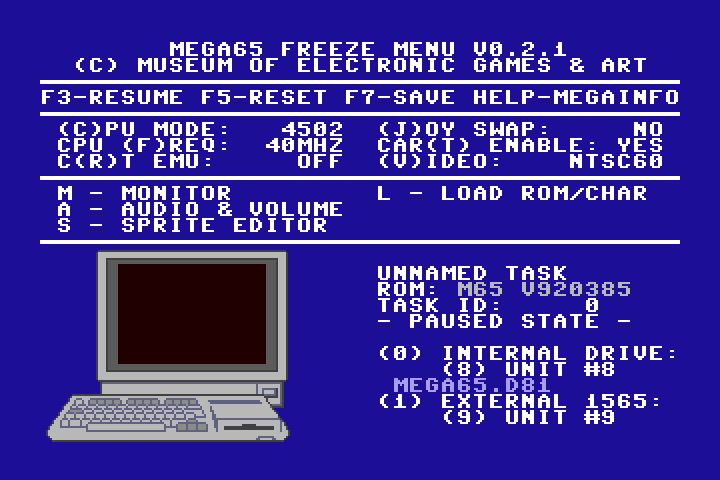
\includegraphics[trim= 10mm 20mm 10mm 20mm,clip,width=0.7\linewidth]{images/freezer.jpg}
\end{center}

The bottom-right part of the Freezer screen shows the current disk drive assignments.
The internal CBDOS which the MEGA65 uses supports up to two
3.5" disk drives and .d81 images, in any combination.
Drive 0 can be assigned to the internal floppy disk drive or a .d81 disk image,
whereas Drive 1 can be assigned to an external floppy disk drive (connected to the
same ribbon cable as the internal drive), or a .d81 disk image.

\index{Disk Drives!Assignment}
A typical configuration is usually one of the following:
\begin{center}
\begin{tabular}{|l|l|l|}
\hline
{\bf Drive 0 Assignment} & {\bf Drive 1 Assignment} \\
\hline
Internal floppy disk drive &  Disk image \\
Disk image                 &  Disk image \\
\hline
\end{tabular}
\end{center}

The assignment, and mounting of disk images can be performed by pressing
\megakey{0} for drive 0, or \megakey{1} for drive 1.

You may have noticed that the drive numbers here (0-1) are different to the more commonly used {\bf UNIT}
numbers (8-9), which you may be more used to. The drive numbers of 0 and 1 are used internally by CBDOS.
However, {\bf BASIC} and Kernal address these storage devices by {\bf UNIT} numbers. CBDOS emulates two single drives for
the operating system, by assigning separate unit numbers to drive 0 and drive 1.
The default assignment is:

\begin{center}
\begin{tabular}{|l|l|l|}
\hline
{\bf Unit/Drive} & {\bf Assignment} \\
\hline
UNIT 8, DRIVE 0  & Internal drive 0 (internal floppy or disk image) \\
UNIT 9, DRIVE 0 & Internal drive 1 (external floppy or disk image) \\
\hline
\end{tabular}
\end{center}


You may wish to change this unit assignment, if for example
a 1541 drive is connected to the IEC port as unit 8.
In this case, the internal drive assignment can be switched to an alternative unit
to avoid conflict. To do this, press \megakey{8} to toggle the unit assignment of drive 0
between 8 and 10, and \megakey{9} to toggle the unit assignment of drive 1, between 9 and 11.

After setting the preferences, the Freezer can be exited
with \megakey{F3}. The Freezer restores the screen and
returns to the interrupted program.

Note: The drive and unit assignments are temporary, and will be reset to their defaults
after power down or reset. For permanent settings, use the {\bf CONFIGURE}
menu. You can read more about this menu on page \pageref{configuring-chipset}.

\index{Disk Drives!D81 Images}
\section{Using D81 images}
As previously mentioned, the MEGA65 allows the use of D81 files instead of using physical disks. The MEGA65 includes a
built-in file browser, which allows you to choose which D81 file to mount. To do this, enter the Freezer menu,
then press \megakey{0} or \megakey{1}, to choose the drive to mount it to.

When you do this, the file browser will appear:

\begin{center}
\includegraphics[trim= 10mm 20mm 10mm 20mm,clip,width=0.7\linewidth]{images/d81-file-browser.png}
\end{center}

The file browser will list all D81 images on the microSD card. The MEGA65 prioritises the external microSD card, so if you
prefer to use an image on the internal SD card, the microSD card should be removed (when doing this, the MEGA65 needs
to be reset as well).

Press the cursor keys to choose a file. If the currently selected file isn't a valid D81, the border will be red,
otherwise it will be blue, as shown above. Whilst browsing for D81 files, the list of files within the currently
selected D81 file will be shown on the right-hand side.

When you find the D81 file you wish to mount, press \specialkey{RETURN}.
This will take you back to the Freezer menu, and the selected D81 file will be shown under the selected drive.
In the screenshot below, the  \screentext{MEGA65.D81} file has been mounted to drive 0:

\begin{center}
\includegraphics[trim= 10mm 20mm 10mm 20mm,clip,width=0.7\linewidth]{images/freezer-chosen-d81.png}
\end{center}

Next, press \megakey{F3} to exit the Freezer menu and return to the currently running program. Alternatively,
pressing \megakey{F5} will exit the Freezer, and reset the MEGA65 as well.

Now that the file has been mounted, you can use
the {\bf DIR} command to list the files in the image, or any of the {\bf LOAD}, and {\bf SAVE} commands, like you
would on a physical disk.

You may have noticed that the file browser has a \screentext{ - NO DISK - } and \screentext{ - INTERNAL 3.5" - }
entry. These are used for un-mounting a D81 image - but with a difference. \screentext{ - NO DISK - } is used to tell
the MEGA65 that no disk is inserted, and to not try and find one when performing a disk-based operation. On the other
hand, \screentext{ - INTERNAL 3.5" - } is used when using a physical 3.5" disk in the internal drive. If no disk is
inserted and a disk-based operation is performed with the \screentext{ - INTERNAL 3.5" - } option, the MEGA65 will
try and find a disk, which could take a few seconds.


\subsection{Auto booting from a disk}
If you would like the MEGA65 to automatically perform any BASIC commands upon startup, you can create an
\screentext{AUTOBOOT.C65} PRG file on your disk/image. In this file, you can write BASIC programs to do things such
as changing the {\bf BACKGROUND}, {\bf BORDER}, or {\bf FOREGROUND} colours, or even {\bf LOAD} a program.

For example, to change the background and border colours to black, and load a program called \screentext{MYPROGRAM}
automatically, create a BASIC listing like the following, then {\bf SAVE} it:


\begin{tcolorbox}[colback=black,coltext=white]
\verbatimfont{\codefont}
\begin{verbatim}
10 BACKGROUND 0
20 BORDER 0
30 LOAD "MYPROGRAM.PRG"
SAVE "AUTOBOOT.C65"
\end{verbatim}
\end{tcolorbox}

\subsection{Saving D81 file settings}

The D81 settings are temporary, and will be reset to their defaults after power down. You can change the default settings
in the {\bf CONFIGURE} menu. When opening the Configure menu, press the \megakey{F1} and \megakey{F2} keys
to reach the \screentext{CHIPSET} section, then navigate to the \screentext{F011 DISK CONTROLLER} options.
Select the \screentext{USES SDCARD DISK IMAGE} setting, then enter the name of the disk image you wish to have mounted
by default in the \screentext{DEFAULT DISK IMAGE} field. A screenshot showing these settings with
\screentext{MEGA65.D81} as the default D81 disk image is shown below:

\begin{center}
\includegraphics[width=0.7\linewidth]{images/ss-m65config-2.png}
\end{center}

You can read more about the Configure menu on page \pageref{sec:configuration-utility}.


%\part{FIRST STEPS IN CODING}
%\chapter{Getting Started in BASIC}
\label{cha:basic-getting-started}

It is possible to code on the MEGA65 in many languages,
however most people start with BASIC.  That makes sense,
because BASIC stands for Beginner's All-purpose Symbolic
Instruction Code: It was made for people like you to get
started with in the world of coding!

A few short words before we dive in: BASIC is a programming
language, and like spoken language it has conventions, grammar
and vocabulary.  Fortunately, it is much quicker and easier
to learn than our complex human languages. But if you pay
attention, you might notice some of these structures, and that
can help you along your path in the world of coding.

If you haven't already read \bookvref{cha:getting-started},
it might be a good idea to do so. This will help you be able to
more confidently interact with the MEGA65 computer.

It's also great to remember that if you really confuse the MEGA65,
you can always get back to the READY. prompt by just pressing the
reset button on the left-hand side of the keyboard, or if that
doesn't help, then by turning it off
and on again using the power switch on the left-hand side of the keyboard.
You don't have to worry about shutting the computer
down properly or any of that nonsense.  The only thing to remember
is that if you had any unsaved work, it will be lost when you switch
the computer off and on again or press the reset button.

Finally, if you don't understand all of the descriptions and information
with an example -- don't worry! We have provided as much information
as we can, so that it is there in case you have questions, encounter problems are
just curious to discover more.  Feel free to skip ahead to the examples
and try things out, and then you can go back and re-read it when you are motivated
to find something out, or help you work though a problem.  And if you don't find
the answer to your problem, send us a message!  There are support forums for the
MEGA65 at \url{https://mega65.net}, and you can
report problems with this guide at:

\url{https://github.com/mega65/mega65-user-guide}

We hope you have as much fun learning to program the MEGA65 as
we have had making it!

\section{Your first BASIC programs}

The MEGA65 was designed to be programmed! When you switch it on,
it takes a couple of seconds to get its house in order, and then
it quickly shows you a ``READY.'' prompt and flashing block called
the cursor.  When the cursor is blinking, it tells you that the
computer is waiting for input.  The ``READY.'' message tells you
that the BASIC programming language is running and ready for you to
start programming.  You don't even need to load any programs --
you can just get started.

\needspace{4cm} % Dont allow following paragraph to separate from
                % following element
Try typing the following into the computer and see what happens:

\begin{screenoutput}
HELLO COMPUTER
\end{screenoutput}

\needspace{4cm} % Dont allow following paragraph to separate from
                % following screenshot

To do this, just type the letters as you see them above.  The computer
will already be in uppercase mode, so you don't need to hold \specialkey{SHIFT}
or \specialkey{CAPS\\LOCK} down.  When you have typed "HELLO COMPUTER", press
  \specialkey{RETURN}.  This tells the computer you want it to accept the
  line of input you have typed.  When you do this, you should see a message something
  like the following:

\screenshotwrap{images/getting-started/syntax-error.png}

  If you saw a \screentextwide{SYNTAX ERROR} message something like that one, then congratulations:
  You have succeeded in communicating with the computer!\index{Errors!Syntax}\index{SYNTAX ERROR}
  Error messages sound much nastier than they are.  The MEGA65 uses them, especially
  the syntax error to tell you when it is having trouble understanding what you have
  typed, or what you have put in a program.  They are nothing to be afraid of, and
  experienced programmers get them all the time.

  In this case, the computer was confused because it doesn't understand the word
  ``hello'' or the word ``computer''.  That is, it didn't know what you wanted it to
  do.  In this regard, computers are quite stupid. They know only a few words, and
  aren't particularly imaginative about how they interpret them.

\needspace{4cm} % Dont allow following paragraph to separate from
                % following screenshot

So let's try that again in a way that the computer will understand.  Try typing
  the following in.  You can just type it right away. It doesn't matter that the
  syntax error message can still be seen on the screen.  The computer has already
  forgotten about that by the time it told you \screentextwide{READY.} again.

\begin{screenoutput}
PRINT "HELLO COMPUTER"
\end{screenoutput}

Again, make sure you don't use shift or shift-lock while typing it in.  The symbols around
the words \screentextwide{HELLO COMPUTER} are double-quotes.  If you are used to an Australian or American
keyboard, you might discover that they double-quote key is in a rather different place to
where you are used to:  Double-quotes can be typed on the MEGA65 by holding down
\specialkey{SHIFT}, and then pressing \megakey{2}.  Don't forget to press \specialkey{RETURN}
when you are done, so that the computer knows you want it to do something with your input.

If you make a mistake while typing, you can use \specialkey{INST\\DEL} to rub out the mistake
and fix it up.  You can also use the cursor keys to move back and forth on the line while
you edit the line you are typing, but there is a bit of a trick if you have already typed
a double-quote: If you try to use the cursor keys, it will print a funny reversed symbol
instead of moving the cursor.  This is because the computer thinks you want to record
moving the cursor in the text itself, which can be really useful and fun, and which you can
read more about in \bookvref{cha:getting-started}. But for now, if you
make a mistake just press \specialkey{RETURN} and type the messed up line again.

\needspace{4cm} % Dont allow following paragraph to separate from
                % following screenshot
Hopefully now you will see something like the following:

\screenshotwrap{images/getting-started/print-hello-computer.png}

  This time no new \screentextwide{SYNTAX ERROR} message should appear. But if some kind
  of error message has appeared, just try typing in the command again, after
  taking a close look to work out where the mistake might be.

  Instead of an error, we should see \screentextwide{HELLO COMPUTER} repeated underneath
  the line you typed in.  The reason this happened is that the computer
  does understand the word \screentextwide{PRINT}.  It knows that whatever comes after
  the word \screentextwide{PRINT} should be printed to the screen.  We had to put \screentextwide{HELLO
  COMPUTER} inside double-quotes to tell the computer that we want it to be
  printed literally.

  If we hadn't put the double-quotes in, the computer would have thought
  that \screentextwide{HELLO COMPUTER} was the name of a stored piece of information.
  But because we haven't stored any piece of information in such a place,
  the computer will have zero there, so the computer will print the number
  zero. If the computer prints zero or some other number when
  you expected a message of some sort, this can be the reason.

\needspace{4cm} % Dont allow following paragraph to separate from
                % following screenshot
  You can try it, if you like, and you should see something like the following:

  \screenshotwrap{images/getting-started/print-hello-computer-no-quotes.png}

  In the above examples we typed commands in directly, and the computer executed
  them immediately after you pressed \specialkey{RETURN}.  This is why
  typing commands in this way is often called {\em direct mode} or {\em immediate mode}.

  But we can also tell the computer to remember a list of commands to execute one
  after the other.   This is done using the rather unimaginatively named {\em non-direct mode}.
  To use non-direct mode, we just put a number between 0 and 63999 at the start of
  the command.  The computer will then remember that command.  Unlike when we executed
  a direct-mode command, the computer doesn't print \screentextwide{READY.} again. Instead the cursor
  just reappears on the next line, ready for us to type in more commands.

\needspace{4cm} % Dont allow following paragraph to separate from
                % following screenshot
  Let's try that out with a simple little program.  Type in the following three lines of
  input:

\begin{screenoutput}
1 FOR I = 1 TO 10 STEP 1
2 PRINT I
3 NEXT I
\end{screenoutput}
\index{FOR}
\index{BASIC 65 Commands!FOR}

\needspace{4cm} % Dont allow following paragraph to separate from
                % following screenshot
When you have done this, the screen should show something like this:

\screenshotwrap{images/getting-started/first-steps-for-loop-programme-1.png}

If it doesn't you
can try again. Don't forget, if you feel that the computer is getting all muddled up,
you can just press the reset button or flip the power switch off and on, at the left-hand side of the
computer to reboot it. This only takes a couple of seconds, and doesn't hurt the MEGA65
in anyway.

We have told the computer to remember three commands, that is, \screentextwide{FOR I = 1 TO 10 STEP 1},
\screentextwide{PRINT I}
and \screentextwide{NEXT I}.  We have also told the computer which order we would like to run them in: The
computer will start with the command with the lowest number, and execute each command that
has the next higher number in turn, until it reaches the end of the list.  So it's a bit like
a reminder list for the computer. This is what we call a program, a bit like the program at
a concert or the theatre, it tells us what is coming up, and in what order.
So let's tell the computer to execute this program.

But first, let's try to guess what will happen.  Let's start with the middle command, \screentextwide{PRINT I}.
We've seen the \screentextwide{PRINT} command, and we know it tells the computer to print things to the screen.
The thing it will try to print is \screentextwide{I}.  Just like before, because there are no double-quotes
around the \screentextwide{I}, it will try to print a piece of stored information.  The piece of information
it will try to print will be the piece associated with the thing \screentextwide{I}.

When we give a piece of
information like this a name, we call it a {\em variable}\index{variable}.  They are called
variables because they can vary.  That is, we can replace the piece of information associated
with the variable called I with another piece of information.  The old piece will be forgotten
as a result.  So if we gave a command like \screentextwide{LET I = 3}, this would replace whatever was stored
in the variable called \screentextwide{I} with the number 3.

Back to our program, we now know that the 2\textsuperscript{nd} command will try to print the piece of information
stored in the variable \screentextwide{I}.  So lets look at the first command: \screentextwide{FOR I = 1 TO 10 STEP 1}.  Although
we haven't seen the \screentextwide{FOR} command before, we can take a bit of a guess at how it works. It looks like
it is going to put something into the variable \screentextwide{I}.  That something seems to have something to do
with the range of number 1 through 10, and a step or interval of 1.  What do you think it will do?

If you guessed
that it will put the values 1, 2, 3, 4, 5, 6, 7, 8, 9 and then 10 into the variable \screentextwide{I}, then you
can give yourself a pat on the back, because that's exactly what it does.  It also helps us to
understand the 3\textsuperscript{rd} command, \screentextwide{NEXT I}: That command tells the computer to put the next value into
the variable \screentextwide{I}.  And here is a little bit of magic: When the computer does that, it goes back
up the list of commands, and continues again from the command after the \screentextwide{FOR} command.

So lets pull that together: When the computer executes the first command, it discovers that it has
to put 10 different values into the variable \screentextwide{I}. It starts by putting the first value in there, which
in this case will be the number 1.
The computer then continues to the second command, which tells the computer to print the piece of
information that is currently stored in the variable called \screentextwide{I}. That will be the number 1, since
that was the last thing the computer was told to put there.  Then the computer proceeds to the
third command, which tells it that it is time to put the next value into the variable \screentextwide{I}.  So the
computer will throw away the number 1 that is currently in the variable \screentextwide{I}, and put the number 2 in
there, since that is the next number in the list.  It will then continue from the 2\textsuperscript{nd} command,
which will cause the computer to print out the contents of the variable \screentextwide{I} again.  Except that this
time \screentextwide{I} has had the number 2 stored in it most recently, so the computer will print the number 2.
This process will repeat, until the computer has printed all ten values that the \screentextwide{FOR} command
indicated it to do.

\needspace{4cm} % Dont allow following paragraph to separate from
                % following screenshot
To see this in action, we need to tell the computer to execute the program of commands we typed in.
We do this by using the \screentextwide{RUN} command. Because we want it to run the program immediately, we
should use immediate mode (remember, this is another name for direct mode).
So just type in the word \screentextwide{RUN} and press \specialkey{RETURN}.  You should then see a display
that looks something like the following:

\screenshotwrap{images/getting-started/first-steps-for-loop-programme-1-running.png}

  You might notice a couple of things here:

  First, the computer has told us it is \screentextwide{READY.} again
  as soon as it finished running the program. This just makes it easier for us to know when we
  can start giving commands to the computer again.

  Second, when the computer got to the bottom of the screen
  it automatically scrolled the display up to make space.  This is quite normal.  What is important
  to remember, is that the computer forgets everything that scrolls off the top.  The only exception
  is if you have told the computer to remember a command by putting a number in front of it.  So
  our program is quite safe for now. We can see that this is the case by typing the \screentextwide{RUN} command a
  couple more times: The program listing will have scrolled off the top of the screen, but we can
  still RUN the program, because the computer has remembered it.  Give it a try!
  Did it work?

\needspace{4cm} % Dont allow following paragraph to separate from
                % following screenshot
  If you wish to see the program of remembered commands, you can use the \screentextwide{LIST}\index{LIST}\index{BASIC 65 Commands!LIST}
  command.  This commands causes the computer to display the remembered program of commands to the screen, like in the display here.
  If you would like to replace any of the commands in the program, you can type a new line that has the same number as the one you
  wish to change.

\screenshotwrap{images/getting-started/first-steps-for-loop-programme-1-listing.png}

\needspace{4cm} % Dont allow following paragraph to separate from
                % following screenshot
  For example, to print the results all on one line, we could modify the second line of the program to \screentextwide{PRINT I;} by
  typing the following line of input and pressing \specialkey{RETURN}:



\begin{screenoutput}
2 PRINT I;
\end{screenoutput}

\index{PRINT}
\index{BASIC 65 Commands!PRINT}
%\end{tcolorbox}

\needspace{4cm} % Dont allow following paragraph to separate from
                % following screenshot

You can make sure that the change has been remembered by running the \screentextwide{LIST} command again, as we can see here.
You can then use the \screentextwide{RUN} command to run the modified
program, like this:

\screenshotwrap{images/getting-started/first-steps-for-loop-programme-1-modified.png}

It is quite easy to modify your programs in this way.  As you become more comfortable with the process, there are two
additional helpful tricks:

First, you can give the {\bf LIST} command the number of a command, or line as they are referred to, and it will display only
that line of the program.  Alternatively, you can give a range separated by a minus sign to display only a section of the program,
e.g., \screentextwide{LIST 1 - 2} to list the first two lines of our program.

Second, you can use the cursor keys to move the cursor to a line which has already been remembered and is displayed on the screen. If you
modify what you see on the screen, and then press \specialkey{RETURN} while the cursor is on that line, the BASIC interpreter will
read in the modified line and replace the old version of it.  It is important to note that if you modify multiple lines of the program
at the same time, you must press \specialkey{RETURN} on each line that has been modified. It is good practice to check that the
program has been correctly modified. Use the {\bf LIST}\index{LIST}\index{BASIC 65 Commands!LIST} command again to achieve this.


  \subsection{Exercises to try}

  {\bf 1. Can you make it count to a higher or lower number?}

  At the moment it counts from 1 to 10.  Can you change it to count to 20 instead?  Or to count from 3 to 17?
  Or how about from 14.5 to 21.5? What do you think you would need to reverse the order in which it counts?

  {\em Clue:} You will need to modify the \screentextwide{FOR} command.

  {\bf 2. Can you change the counting step?}

  At the moment it counts by ones, i.e., each number is one more than the last.  Can you change it to count by twos
  instead? Or by halves, so that it counts 1, 1.5, 2, 2.5, 3, \ldots?

  {\em Clue:} You will need to modify the \screentextwide{STEP} clause
  of the \screentextwide{FOR} command.\index{STEP}\index{BASIC 65 Commands!STEP}


  {\bf 3. Can you make it print out one of the times tables?}

  At the moment it prints the answers to the 1 times tables, because it counts by ones.
  Can you make it count by threes, and show the three times tables?

  {\em Clue:} You will need to modify the \screentextwide{FOR} command.

  {\bf 4. Can you make it print out the times tables from 1$\times$1 to 10$\times$10?}

  {\em Clue:} You might like to use ; on the end of \screentextwide{PRINT} command, so that you can have
  more than one entry per line on the screen.\\
  {\em Clue:} The \screentextwide{PRINT} command without any argument will just advance to the start of the next line.\\
  {\em Clue:} You might need to have multiple \screentextwide{FOR} loops, one inside the other.

\section{First steps with text and numbers}

In the last section we started to use both numbers and text.  Text on computers is made by stringing individual letters
and other symbols together.  For this reason they are called {\em strings}.  We also call the individual letters and
symbols {\em characters}.  The name character comes from the printing industry where each of the symbols that can be
printed on a page. For computers, it has much the same meaning, and the set of characters that a computer can display
is rather unimaginatively called a {\em character set}.\index{character}\index{character set}\index{string}.

When the MEGA65 expects some for of input, it is typically looking for one of four things:

\begin{enumerate}
\item {\em a keyword} like \screentextwide{PRINT} or \screentextwide{STEP}, which are words that have a special meaning to the computer;
\item {\em a variable name} like \screentextwide{I} or \screentextwide{A\$} that it will then use to either store or retrieve a piece of information;
\item {\em a number} like \screentextwide{42} or \screentextwide{-30.3137}; or
\item {\em a string} like \screentextwide{"HELLO COMPUTER"} or \screentextwide{"23 KILOMETRES"}.
\end{enumerate}

\needspace{4cm} % Dont allow following paragraph to separate from
                % following screenshot
Sometimes you have a choice of which sort of thing you can provide, while other times you have less choice. What
sort of thing the computer will accept depends on what you are doing at the time.  For example, in the previous
section we discovered that when the computer tells us that it is \screentextwide{READY}, that we can give it
a keyword or a number.  Do you think that the computer will accept all four kinds of thing when it says
\screentextwide{READY.}?  We already know that keywords and numbers and keywords can be entered, but what about
variable names or strings?  Let's try typing in a variable name, say \screentextwide{N}, and pressing \specialkey{RETURN},
and see what happens.  And then lets try with a string, say \screentextwide{"THIS IS A STRING"}.

\screenshotwrap{images/getting-started/typing-variable-name-or-string}

You should get a syntax error each time, telling you that the computer doesn't understand the input you have given it.
Let's start with when you typed the variable: If you just tell the computer the name of a stored piece of information,
it doesn't have the foggiest idea what you are wanting it to do.  It's the same when you give it a piece of information,
like a string, without telling the computer what to do with it.

But as we discovered in the last section, we can tell the computer that we want to see the piece of information that is
stored in a variable using the \screentextwide{PRINT} command.  So we could instead type in \screentextwide{PRINT N}, and
the computer would know what to do, and will print the piece of information stored in the variable called \screentextwide{N}.

In fact, using the \screentextwide{PRINT} command is so common, that programmers got annoying having to type in the \screentextwide{PRINT}
command all the time, that they made a short cut: If you type a question mark character, i.e., a \screentextwide{?}, the computer
knows that you mean \screentextwide{PRINT}.  So for example if you type \screentextwide{? N}, it will do the same as typing
\screentextwide{PRINT N}.  Of course, you have to press \specialkey{RETURN} after each command to tell the computer
you want it to process what you typed.  From here on, we will assume that you can remember to do that, without being reminded.

\needspace{4cm} % Dont allow following paragraph to separate from
                % following screenshot
The \screentextwide{?} shortcut also works if you are telling the computer to remember a command as part of a program.
So if you type \screentextwide{1 ? N}, and then \screentextwide{LIST}, you will see \screentextwide{1 PRINT N}, as we can see
in the following screen-shot:

\screenshotwrap{images/getting-started/print-question-mark}

Like we saw in the last section, the variable \screentextwide{N} has not had a value stored in it, so when the computer looks for
what is there, it finds nothing.  Because \screentextwide{N} is a {\em numeric variable}\index{variable!numeric}, when there is
nothing there, this means zero.  If it was a {\em string variable}\index{variable!string}, then it would have found literally nothing.
We can try that, but first we have to explain how we tell the computer we are talking about a string variable.  We do that by
putting a dollar sign character, i.e., a \screentextwide{\$}, on the end of the variable name. So if we put a \screentextwide{\$} on
the end of the variable name \screentextwide{N}, it will refer to a string variable called \screentextwide{N\$}.

\needspace{4cm} % Dont allow following paragraph to separate from
                % following screenshot
We can experiment with these variables by using the hopefully now familiar
\screentextwide{PRINT} command (or the \screentextwide{?} shortcut)
to see what is in the variables. But we need a convenient way to put
values into them.  Fortunately we aren't the first people to want to
put values into variables, and so the
\screentextwide{LET}\index{LET}\index{BASIC 65 Commands!LET} exists.
The \screentextwide{LET} command is used to put a value into a
variable.  For example, we can tell the computer:

\begin{screenoutput}
  LET N = 5.3
\end{screenoutput}

\needspace{4cm} % Dont allow following paragraph to separate from
                % following screenshot
This tells the computer to put the value 5.3 into the variable
\screentextwide{N}.  We can then use the \screentextwide{PRINT}
command to check that it worked.  Similarly, we can put a value into
the variable \screentextwide{N\$} with something like:

\begin{screenoutput}
  LET N$ = "THE KING OF THE POTATO PEOPLE"
\end{screenoutput}

\needspace{4cm} % Dont allow following paragraph to separate from
                % following screenshot
If we try those, we will see something like the following:

\screenshotwrap{images/getting-started/let-command-examples}

\needspace{4cm} % Dont allow following paragraph to separate from
                % following screenshot
We mentioned just before that \screentextwide{N} is a numeric
variable and that \screentextwide{N\$} is a string variable. This
means that we can only put numbers into \screentextwide{N} and
strings into \screentextwide{N\$}.  If we try to put the wrong kind
of information into a variable, the computer will tell us that we have
mis-matched the kind of information with the place we are trying to
put it by giving us a \screentextwide{TYPE MISMATCH
  ERROR}\index{Errors!Type mismatch}\index{Type mismatch error} like
this:

\screenshotwrap{images/getting-started/type-mismatch-errors}

This leads us to a rather important point: \screentextwide{N} and
\screentextwide{N\$} are separate variables, even though they have
similar names.  This applies to all possible variable names: If the
variable name has a \screentextwide{\$} character on the end, it
means it is a string variable quite separate from the similarly named
numeric variable.  To use a bit of jargon, this means that each {\em type}
of variable has their own separate {\em name
  spaces}\index{name spaces}.

(There are also four other variable name
spaces that we haven't talked about yet: integer variables, identified
by having a \screentextwide{\%} character at the end of their name,
e.g., \screentextwide{N\%}, and arrays of numeric, string or integer
variables. But don't worry about those for now.
We'll talk about those a bit later on.)

So far we have only given values to variables in direct mode, or
by using constructions like \screentextwide{FOR} loops.  But we
haven't seen how we can get information from the user when a program
is running.  One way that we can do this, is with the
\screentextwide{INPUT}\index{BASIC 65 Commands!INPUT}\index{INPUT}
command.

\needspace{4cm} % Dont allow following paragraph to separate from
                % following screenshot
\screentextwide{INPUT} is quite easy to use: We just have to say which
variable we would like the input to go into.  For example, to tell the
computer to ask for the user to provide something to put into the
variable \screentextwide{A\$}, we could use something like
\screentextwide{INPUT A\$}.  The only trick with the \stw{INPUT}
command is that it cannot be used in direct mode\index{Direct Mode}.
If you try it, the computer will tell you \stw{ILLEGAL DIRECT
  ERROR}\index{Errors!Illegal Direct}\index{Illegal Direct Error}.
Try it, and you should see something like the following

\screenshotwrap{images/getting-started/illegal-direct-error}

\needspace{4cm}
This means that the \stw{INPUT} command can only be used as part of a
program.  So we can instead do something like the following:

\begin{screenoutput}
1 INPUT A$
2 PRINT "YOU TYPED "; A$
RUN
\end{screenoutput}

\needspace{4cm}
What do you think that this will do?  The first line will ask the
computer for something to put into the variable \stw{A\$}, and the
second line will print the string \stw{"YOU TYPED"}, followed by
what the \stw{INPUT} command read from the user.  Let's try it out:

\screenshotwrap{images/getting-started/input-example-1}

Did you expect that to happen? What is this question mark doing there?
The \stw{?} here is the computer's way of telling you that a
program is waiting for some input from you.  This means that the
computer uses the same symbol, \stw{?}, to mean two different things:
If you type it as part of a program or in direct mode, then it is a
short-cut for the \stw{PRINT} command. That's when you type it. But if
the computer shows it to you, it has this other meaning, that the
computer is waiting for you to type something in. There is also a
third way that the computer uses the \stw{?} character. Have you
noticed what it is?  It is to indicate the start of an error
message. For example, a Syntax Error is indicated by \stw{?SYNTAX
 ERROR}. When a character or something has different meanings in
different situations or contexts, we say that it its {\em context
  dependent}\index{context dependent}.

\needspace{4cm}
But returning to our example,  if we now type
something in, and press \specialkey{RETURN} to tell the
computer that you are done, the program will continue, like this:

\screenshotwrap{images/getting-started/input-example-2}

\needspace{4cm}
Of course, we didn't really know what to type in, because the program
didn't give any hints to the user as to what the programmer wanted
them to do. So we should try to provide some instructions.  For
example, if we wanted the user to type their name, we could print a
message asking them to type their name, like this:

\begin{screenoutput}
  1 PRINT "WHAT IS YOUR NAME"
  2 INPUT A$
  3 PRINT "HELLO "; A$
\end{screenoutput}

\needspace{4cm}
Now if we run this program, the user will get a clue as to what we
expect them to do, and the whole experience will make a lot more sense
for them:

\screenshotwrap{images/getting-started/input-example-3}

When we run the program, we first see the \stw{WHAT IS YOUR NAME} message
from line 1.  The computer doesn't print the double-quote symbols,
because they only told the computer that the piece of information
between them is a string.  The string itself is only the part in
between.

After this we see the \stw{?} character again and the blinking cursor
telling us that the computer is waiting for some input from us.  The
rest of the programmed is {\em blocked}\index{I/O!blocking}\index{blocked} from continuing until it we type the
piece of information.  Once we type the piece of input, the computer
stores it into the variable \stw{A\$}, and can continue.  Thus when it
reaches line 3 of the program, it has everything it needs, and
prints out both the \stw{HELLO} message, as well as the information
stored in the variable called \stw{A\$}.

Notice that the word \stw{LISTER} doesn't appear anywhere in the
program.  It exists only in the variable.  This ability to process
information that is not part of a program is one of the things that
makes computer programs so powerful and able to be used for so many
purposes. All we have to do is to change the input, and we can get
different output.


\needspace{4cm}
For example, with our program we run it again and again, and give it
different input each time, and the
program will adapt its output to what we type. Pretty nifty, right?
Let's have the rest of the crew try it out:

\screenshotwrap{images/getting-started/input-extra-ignored-1}

We can see that each time the program prints out the message
customised with the input that you typed in\ldots Until we get to
\stw{RIMMER, BSC}. As always, Mr. Rimmer is causing trouble.  In this
case, he couldn't resist putting his Bronze Swimming Certificate
qualification on the end of his name.

We see that the computer has
given us a kind of error message, \stw{?EXTRA IGNORED}\index{Extra
  Ignored}\index{Errors!Extra Ignored}\index{Warnings!Extra Ignored}.
The error is not written in red, and doesn't have the word \stw{ERROR}
on the end.  This means that it is a warning, rather than an error.
Because it is only a warning, the program continues.  But something
has happened: The computer has ignored Mr. Rimmer's \stw{BSC}, that
is, it has ignored the extra input.  This
is because the \stw{INPUT} command doesn't really read a whole line
of input. Rather, it reads {\em one piece of information}.  The
\stw{INPUT} command thinks that a piece of information ends at the end
of a line of input, or when it encounters a comma (\stw{,}) or colon
(\stw{:}) character.\index{, (comma)}\index{: (colon)}

\needspace{4cm}
If you want to include one of those symbols, you need to surround the
whole piece of information in double-quotes.  So, if Mr. Rimmer had
read this guide instead of obsessing over the Space Core Directives,
he would have known to type \stw{"RIMMER, BSC"} (complete with the
double-quotes), to have the program
  run correctly.  It is important that the quotes go around the whole
  piece of information, as otherwise the computer will think that the
  first quote marks the start of a new piece of information.  We can
  see the difference it makes below:

  \screenshotwrap{images/getting-started/input-quoting-1}

\needspace{1.5cm}
While this can all be a bit annoying at times, it has a purpose: The
\stw{INPUT} command can be used to read more than one piece of
information.  We do this by putting more than one variable after the
\stw{INPUT} command, each separated by a comma.  The \stw{INPUT}
command will then expect multiple pieces of information.  For example,
we could ask for someone's name and age, with a program like this:

\begin{screenoutput}
  1 PRINT "WHAT IS YOUR NAME AND AGE"
  2 INPUT A$, A
  3 PRINT "HELLO "; A$
  4 PRINT "YOU ARE"; A; " YEARS OLD."
\end{screenoutput}

\needspace{4cm}
If we run this program, we can provide the two pieces of information
on the one line when the computer presents us with the \stw{?} prompt,
for example \stw{LISTER, 3000000}. Note the comma that separates the
two pieces of information, \stw{LISTER} and \stw{3000000}.  It's also
worth noticing that we haven't put any thousands separators into the
number 3,000,000.  If we did, the computer would think we meant three
separate pieces of information, \stw{3}, \stw{000} and \stw{000},
which is not what we meant.  So let's see what it looks like when we
give \stw{LISTER, 3000000} as input to the program:

  \screenshotwrap{images/getting-started/input-multiple-1}

  In this case, the \stw{INPUT}\index{INPUT}
  \index{BASIC 65 Commands!INPUT} command reads the two pieces of
information, and places the first into the variable \stw{A\$}, and the second
into the variable \stw{A}. When the program reaches line 3 it prints
\stw{HELLO} followed by the first piece of information.
Then when it gets to line 4, it prints the string \stw{YOU ARE},
followed by the contents of the variable \stw{A}, which is the number
3,000,000, and finally the string \stw{YEARS OLD}.

It's also possible to just give one piece of information at a time.
In that case, the \stw{INPUT} command will ask for the second piece
of information with a double question-mark prompt, i.e., \stw{??}.
Once it has the second piece of information.  (If we had more than
two variables on the \stw{INPUT} command, it will still present the
same \stw{??} prompt, rather than printing more and more
question-marks.)

\needspace{4cm}
So if we try this with our program, we can see this \stw{?} and
\stw{??} prompts, and how the first piece of information ends up in
\stw{A\$} because it is the first variable in the \stw{INPUT}
command.
The second piece of information ends up in \stw{A} because \stw{A} is
the second variable after the \stw{INPUT} command. Here's how it
looks if we give this input to our program:


\screenshotwrap{images/getting-started/input-multiple-2}

Until now we have been asking the user to input information by using a
\stw{PRINT} command to display the message, and then an \stw{INPUT}
command to tell the computer which variables we would like to have
some information input into.  But, like with the \stw{PRINT} command,
this is something that happens often enough, that there is a shortcut
for it. It also has the advantage that it looks nicer when
running, and makes the program a little shorter. The short cut is to
put the message to show after the \stw{INPUT} command, but before the
first variable.

We can change our program to use this approach.  First, we can
change line 3 to include the prompt after the \stw{INPUT} command.  We
can do this one of two ways: First, we could just type in a new line
3. The computer will automatically replace the old line 3 with the new
one.

But, as we have mentioned a few times now, programmers are lazy
beasts, and so there is a short-cut: If you can see the line on the
screen that you want to change, you can use the cursor keys to
navigate to that line, edit it on the screen, and then press
\specialkey{RETURN} to tell the computer to accept the new version
of the line.\index{Programmes!editing}\index{Programmes!replacing
  lines}\index{Lines!editing}\index{Lines!replacing}

\needspace{4cm}
Either way, you
can check that the changes succeeded by typing the \stw{LIST} command
on any line of the screen that is blank.  This will show the revised
version of the program.  For example:

\screenshotwrap{images/getting-started/replacing-line-1}

\needspace{3cm}
We still have a little problem, though: Line 1 will print the message
\stw{WHAT IS YOUR NAME AND AGE}, and then Line 2 will print it again!
We only want the message to appear once. Thus we would like to change
line 1 so that it doesn't do this any more.  Because there is no other
command on line 1 that we want to keep, that line can just become
empty. So we can type in something like this:

\begin{screenoutput}
1
\end{screenoutput}

\needspace{4cm}
We can confirm that the contents of the line have been deleted by
running the \stw{LIST} command again, like this:

\screenshotwrap{images/getting-started/deleting-line-1}

Did you notice something interesting? When we told the computer to
make line 1 of the program empty, it deleted it completely!
That's because the computer thinks that an empty line is of no use.
It also makes sure that your programs don't get all cluttered up
with empty lines if you make lots of changes to your programs.

It is also possible to DELETE a range of lines. For example (but don't do this now), you could delete lines 3-4 with:

\begin{screenoutput}
  DELETE 3-4
\end{screenoutput}

You can read more about the DELETE command in the BASIC 65 Command Reference.

\needspace{4cm}
With that out the way, let's run our program and see what happens.
As usual, just type in the \stw{RUN} command and press
\specialkey{RETURN}.  You should see something like this:

\screenshotwrap{images/getting-started/input-comma}

\needspace{2.5cm}
We can see our prompt of \stw{WHAT IS YOUR NAME AND AGE} there, but
now the cursor is appearing without any \stw{?} character. This is
because we put a comma (\stw{,}) after the message in the \stw{INPUT}
command.  To get the question mark, we have to instead put a
semi-colon (\stw{;}) after the message, like this:

\begin{screenoutput}
INPUT "WHAT IS YOU NAME AND AGE"; A$, A
\end{screenoutput}

\needspace{4cm}
Now if we run the program, we should see what we are looking for:

\screenshotwrap{images/getting-started/input-semicolon}

  \subsection{Exercises to try}

  {\bf 1. Can you make the program ask someone for their name, and
    then for their favourite colour?}

  At the moment it asks for their name and age. Can you change the
  program so that it reports on their favourite colour instead of
  their age?

  {\em Clue:} What type of information is age? Is it numeric or a
  string? Is it the same type of information as the name of a colour?

  {\bf 2. Can you write a program that asks someone for their name,
    prints the hello message, and then asks for their age and prints
    out that response?}

  \needspace{2cm}
  At the moment, the program expects both pieces of information at
  the same time. This means the program can't print a message about
  the first message until after it has both pieces of information.
  Change the program so that you can have an interaction like the
  following instead:

\begin{screenoutput}
WHAT IS YOUR NAME? DEEP THOUGHT
HELLO DEEP THOUGHT
WHAT IS THE ANSWER? 42
YOU SAID THE ANSWER IS 42
\end{screenoutput}

{\em Clue:} You will need more lines in your program, so that you
can have more than one \stw{INPUT} and \stw{PRINT} command.

{\bf 3. Can you write a program that asks several questions, and
  then prints out the list of answers given?}

\needspace{2cm}
Think of several questions you would like to be able to ask someone,
and then write a program that asks them, and remembers the answers
and prints them out with an appropriate message. For example, running
your program could look like this:

\begin{screenoutput}
  WHAT IS YOUR NAME? FRODO
  HOW OLD ARE YOU? 33
  WHAT IS YOUR FAVOURITE FOOD? EVERYTHING!
  THANK YOU FOR ANSWERING.
  YOUR NAME IS FRODO
  YOU ARE 33 YEARS OLD
  YOU FAVOURITE FOOD IS EVERYTHING!
\end{screenoutput}

{\em Clue:} You will need more lines in you program, to have the
various \stw{INPUT} and \stw{PRINT} commands.

{\em Clue:} You will need to think carefully about which variable
names you will use.

\section{Making simple decisions}

In the previous section we have learnt how to input text and numeric
data, and how to display it.  However, the programs have just
followed the lines of instruction in order, without any way to decide
what to do, based on what has been input.

In this section we will see how we can take simple decisions using the
\stw{IF}\index{IF}\index{BASIC 65 Commands!IF} and
\stw{THEN}\index{THEN}\index{BASIC 65 Commands!THEN} commands.
The \stw{IF} command checks if something is true or false, and if it
is true, causes the computer to execute the command the comes after
the \stw{THEN} command.

The way the computer decides whether something is true or false is
that it operates on the supplied information using one of several
symbols. These symbols are thus called {\em operators}.  Also, because
the compare two things, they depend on the relationship of the
things.  For this reason they are called {\em relational}
operators.\index{relational operators}\index{operators!relational}
They include the following:

\begin{itemize}
  \item Equals (\stw{=}). For example, \stw{3 = 3} would be true,
    while \stw{3 = 2} would be false.
  \item Less than (\stw{<}). For example, \stw{1 < 3} would be true,
    while both \stw{3 < 3} and \stw{1 < 3} would be false.
  \item Greater than (\stw{>}). For example, \stw{3 > 1} would be
    true, while both \stw{3 > 3} and \stw{1 > 3} would be false.
\end{itemize}

As it is common to want to consider when something might be equal or
greater than, or equal or less than, there are short cuts for
this. Similarly, if you wish to test if something is not equal to
something else, there is a relational operator for this, too:

\begin{itemize}
\item Unequal, which we normally say as {\em not equal}\index{not
  equal}\index{unequal}\index{<> (not equal to)}
  (\stw{<>}). This is different to the mathematical symbol for not
  equal, $\ne$, because the MEGA65's character set does not include a
  character that looks like that. So the programmers who created BASIC
  for the MEGA65 used the greater than and less than signs together
  to mean either less than or greater than, that is, not equal to.
  For example, \stw{1 <> 3} would be true,
    while \stw{3 <> 3} would be false.
  \item Less than or equal to (\stw{<=}). For example, \stw{1 < 3} and
    \stw{3 <= 3} would be true,
    while both \stw{4 < 3} would be false.
  \item Greater than or equal to (\stw{>=}). For example, \stw{3 >= 1}
    and \stw{3 >= 3} would be
    true, while both \stw{1 >= 3} would be false.
\end{itemize}

A good trick if you have trouble remembering which way the \stw(<) and \stw(>)
signs go, the side with more ends of lines is the one that needs to
have more. For example, the \stw(<) symbol has one point on the left, but
two ends of lines on the right-hand side.  So for something to be true
with \stw(<), the number on the left-hand side needs to be less than the number
on the right-hand side.  This trick even works for the equals sign, \stw(=),
because it has the same number of ends on both sides, so you can
remember that the numbers on both sides need to be equal.  It also
works when you have two symbols together, like \stw(>=), it is true if
the condition is true for any of the symbols in it. So in this case
the \stw(>) symbol has more ends on the left than the right, so if the
number on the left is bigger than the number on the right, it will be
true. But also because the \stw(=) symbol has two ends on each side,
it will be true if the two numbers are the same.

\needspace{2cm}
Using these relational operators, we can write a line that will do
something, but only if something is true or false.  Let's try this
out, with a few examples:

\begin{screenoutput}
  IF -2 < 0 THEN PRINT "-2 IS A NEGATIVE NUMBER"
  IF 2 < 0 THEN PRINT "2 IS A NEGATIVE NUMBER"
  IF 0 < -2 THEN PRINT "-2 IS A POSITIVE NUMBER"
  IF 0 < 2 THEN PRINT "2 IS A POSITIVE NUMBER"
\end{screenoutput}

\needspace{4cm}
These commands work fine in direct mode, so you can just type them
directly into the computer to see what they will do.  This can be
handy for testing whether you have the logic correct when planning an
\stw{IF} -- \stw{THEN} command.  If you type in those commands, you
should see something like the following:

\screenshotwrap{images/getting-started/if-then-less-than-examples}

We can see that only the \stw{PRINT} commands that followed an
\stw{IF} command that has a true value were executed. The rest
were silently ignored by the computer.  But we can of course include
these into a program. So lets make a little program that will ask
for two numbers, and say whether they are equal, or if one is greater
or less than the other.  Before you have a look at the program, have
a think about how you might do it, and see if you can figure it out.
The clue we will give you, is that the \stw{IF} command also accepts the name of
a variables, not just numbers. So you can do something like \stw{IF A
  > B THEN PRINT "SOMETHING"}. The program will be on the next page, to stop you peeking before you
have a think about it!

\pagebreak

Did you have a go?  There are lots of different ways it could be done,
but here is what we came up with:

\begin{screenoutput}
1 INPUT "WHAT IS THE FIRST NUMBER"; A
2 INPUT "WHAT IS THE SECOND NUMBER"; B
3 IF A = B THEN PRINT "THE NUMBERS ARE EQUAL"
4 IF A > B THEN PRINT "THE FIRST NUMBER IS BIGGER"
5 IF B > A THEN PRINT "THE SECOND NUMBER IS BIGGER"
\end{screenoutput}

We can then run the program as often as we like, and the computer
can tell us which of the two numbers we give it is biggest, or if they
are equal:

\screenshotwrap{images/getting-started/if-compare-variables-1}

Notice how in this program, we didn't use fixed numbers in the
\stw{IF} command, but instead gave variable names instead.  This is
one of the very powerful things in computer programming, together
with being able to make decision based on data. By being able to refer
to data by name, regardless of its current value or how it got there,
lets the programmer create very flexible programs.

Let's think about a bit of a more interesting example: a ``guess the
number'' game.\index{Guess the number}\index{Games!Guess the number}
For this, we need to have a number that someone has to guess, and then
we need to accept guesses, and indicate whether the guess was correct
or not. If the guess is incorrect, we should tell the user if the
correct number is higher or lower.

We have already learned most the ingredients to make such a program: We
can use \stw{LET} to set a variable to the secret number, \stw{INPUT}
to prompt the user for their guess, and then \stw{IF}, \stw{THEN} and
\stw{PRINT} to tell the user whether their guess was correct or not.
So let's make something. Again, if you like, stop and think and
experiment for a few minutes to see if you can make such a program
yourself.

Here is how we have done it.  But don't worry if you have done it in a
quite different way: There are often many ways to write a program to
perform a particular task.

\begin{screenoutput}
1 SN=23
2 PRINT "GUESS THE NUMBER BETWEEN 1 AND 100"
3 INPUT "WHAT IS YOUR GUESS"; G
4 IF G<SN THEN PRINT "MY NUMBER IS BIGGER"
5 IF G>SN THEN PRINT "MY NUMBER IS SMALLER"
6 IF G=SN THEN PRINT "CONGRATULATIONS! YOU GUESSED MY NUMBER!"
\end{screenoutput}

\needspace{4cm}
The first line puts our secret number into the variable \stw{SN}.
The second line prints a message telling the user what they are
supposed to do. The third line asks the user for their guess, and puts
it into the variable \stw{G}. The
fourth, fifth and sixth lines then check whether the guess is correct
or not, and if not, which message it should print. This is done by
using the \stw{IF} command and an appropriate relative operator to
make each decision.  This works well, to a point. For example:

\screenshotwrap{images/getting-started/guess-number-1}

We can see that it prints the message, and it asks for a guess, and
responds appropriately. But if we want to guess again, we have to use
the \stw{RUN} command again for each extra guess. That's a bit poor
from the user's perspective. However that is unlikely to be a problem
for long, because the user can see the secret number in the listing on
the screen!

So we would like to fix these problems.  Let's start with hiding the
listing.  We previously mentioned that when the screen scrolls,
anything that was at the top of the screen disappears.  So we could
just make sure the screen scrolls enough, that any listing that was
visible is no longer visible. We could do this using \stw{PRINT} and a
\stw{FOR} loop.  The screen is 25 lines, so we could do something
like:

\begin{screenoutput}
FOR I = 1 to 25
PRINT
NEXT I
\end{screenoutput}

But there are better ways.  If you hold down \specialkey{SHIFT},
and then press \specialkey{CLR\\HOME}, it clears the
screen.  This is much simpler and more convenient. But how can we do
something like that in our program?  It turns out to be very simple:
You can type it while entering a string!  This is because the keyboard
works differently based on whether you are in {\em quote
  mode}\index{quote mode}.

Quote mode is just a fancy way of
describing what happens when you type a double-quote character into
the computer: Until you type another double-quote or press the
\specialkey{RETURN}.  You might remember we mentioned the problem of
funny symbols coming up when using the cursor keys. We didn't want to
distract you at the time, but that is a symptom of being in quote mode:
In quote mode many special keys show a symbol that represents them,
rather than taking their normal action.  For example, if you press the
cursor left key while in quote mode, a \stw{Ƣ} symbol appears. If you
press the cursor right key, a \stw{Ž}, up \stw{Ʊ}, down \stw{ű} and the
\specialkey{CLR\\HOME} a \stw{ų}, and if you are holding down
\specialkey{SHIFT} and press \specialkey{CLR\\HOME} a \stw{Ƴ}.

\needspace{3cm}
So let's use this to make the second line clear the screen when it
prints the \stw{GUESS THE NUMBER BETWEEN 1 AND 100} message.  The
first time you try it is a bit confusing, but once you get the hang of
it, it is quite easy.  What we want in the end is a line that looks
like this:

\begin{tcolorbox}[colback=black,coltext=white]
\verbatimfont{\codefont}
\begin{verbatim}
2 PRINT "ƳGUESS THE NUMBER BETWEEN 1 AND 100"
\end{verbatim}
\end{tcolorbox}

To do this, start by typing \stw{2 PRINT "}.  Then hold the
\specialkey{SHIFT} key down, and press \specialkey{CLR\\HOME}.
Your line should now look like \stw{2 PRINT"Ƴ}.  If so, you have
succeeded! You can now finish typing the line as normal.  When you
have done that, you can use the \stw{LIST} command as usual, to make
sure that you have successfully modified the program.   You should
see your modified line with the \stw{Ƴ} symbol in it.

\screenshotwrap{images/getting-started/guess-number-2}

\needspace{2cm}
If you now run the program by typing in \stw{RUN} and pressing
\specialkey{RETURN} as usual, the 2\textsuperscript{nd} line tells
the compute to clear the screen before printing the rest of the message, like this:

\screenshotwrap{images/getting-started/guess-number-3}

This hides the listing from the user, so that they can't immediately see
what our secret number is. We can type our guess in, the same as before,
but just like before, after one guess it returns to the \stw{READY.}
prompt.  We really would like people to be able to make more than one
guess, without needing to know that they need to run the program
again.

\needspace{3cm}
There are a few ways we could do this. We already saw the \stw{FOR} --
\stw{NEXT} pattern. With that, we could make the program give the
user a certain number of guesses.  If we followed the \stw{NEXT}
command with another program line, we could even tell the user when
they have taken too many guesses.  So lets have a look at our
program and see how we might do that.  Here is our current listing again:

\begin{screenoutput}
1 SN=23
2 PRINT "ƳGUESS THE NUMBER BETWEEN 1 AND 100"
3 INPUT"WHAT IS YOUR GUESS"; G
4 IF G<SN THEN PRINT "MY NUMBER IS BIGGER"
5 IF G>SN THEN PRINT "MY NUMBER IS SMALLER"
6 IF G=SN THEN PRINT "CONGRATULATIONS! YOU GUESSED MY NUMBER!"
\end{screenoutput}

If we want the user to have multiple guesses, we need to have lines 2
through 6 run multiple times.  This makes our life a bit tricky,
because it means we need to insert a line between line 1 and 2. But
unless you are a mathemagican, there are no whole numbers between 1
and 2, and the MEGA65 doesn't understand line numbers like 1.5.

\needspace{4cm}
Fortunately, the MEGA65 has the
\stw{RENUMBER}\index{RENUMBER}\index{BASIC 65 Commands!RENUMBER}
\index{Lines!renumbering}
command.  This command can be typed only in direct mode. When
executed, it changes the line numbers in the program, while keeping
them in the same order.  The new numbers are normally multiples of 10,
so that you have lots of spare numbers in between to add extra lines.
For example, if we use it on our program, it will renumber the lines
to 10, 20, \ldots, 60. We can see that this has happened by using the
\stw{LIST} command:

\screenshotwrap{images/getting-started/renumber-1}

\needspace{3cm}
Now our life is much easier: We can choose any  number that is between
10 and 20 to put our \stw{FOR} command into.  It's a common choice to
use the middle number, so that if you think of other things you want
to add in later, you have the space to do it.  So let's add a
\stw{FOR} command to give the user 10 chances to guess the number.  We
can use any variable name we like for this, except for \stw{G} and
\stw{SN}, because we are using those. It would be very confusing if we
mixed those up!  So lets add a line like this:

\begin{screenoutput}
15 FOR I = 1 TO 10 STEP 1
\end{screenoutput}

\needspace{3cm}
Now we need a matching \stw{NEXT I} after line 60.  Let's keep the
nice pattern of adding 10 to work out the next line number, and put it
as line 70:

\begin{screenoutput}
70 NEXT I
\end{screenoutput}

\needspace{4cm}
We can type those lines in, and then use \stw{LIST} command to make
sure the result is correct:

\screenshotwrap{images/getting-started/guess-number-4}

That's looking pretty good.  But there are a couple of little problems still.
Can you work out what they might be? What will happen now after the user makes a guess?
What will happen if they run out of guesses?

If you worked out that making a guess that the screen will be
immediately cleared, you can give yourself a pat on the back! The user
will hardly have time to see the message. Worse, if they guess the
number correctly, they won't know, and the program will keep going.
We'd really like the program to stop or end, once the user makes a
correct guess.

\index{STOP}\index{BASIC 65 Commands!STOP}
\index{END}\index{BASIC 65 Commands!END}
\index{CONT}\index{BASIC 65 Commands!CONT}
We can do this using either the \stw{STOP} or
\stw{END} commands.  These two commands are quite similar.  The main
difference is that if you \stw{STOP} a program, the computer tells
you where it has stopped, and you have the chance to continue the
program using the \stw{CONT} command.  The \stw{END} command, on the
other hand, tells the computer that the program has reached its end,
and it should go back to being \stw{READY}.  The \stw{END} command
makes more sense for our program, because after the user has guessed
the number, there isn't any reason to continue.

Now we need a way to be able tell the computer to do two different
things when the user makes a correct guess. We could just add an extra
\stw{IF} command after line 60 which prints the congratulations
message, e.g., \stw{65 IF G=SN THEN END}.

But we can be a bit more
elegant than that: There is a way to have multiple commands on a
single line.  If you remember back to when we were learning about the
\stw{INPUT} command, you might remember that there were two different
characters that separate pieces of information: \stw{,} and\index{, (comma)}
\stw{:}\index{: (colon)}. The second one, \stw{:}, is called a colon, and can also be
used to separate BASIC commands on a single line.  So if we want to
change line 60 to \stw{PRINT} the message of congratulations and then
\stw{END} the program, we can just add \stw{: END} to the end of the
line. The line should look like this:\index{: (colon)}

\begin{screenoutput}
  60 IF G=SN THEN PRINT "CONGRATULATIONS! YOU GUESSED MY NUMBER!": END
\end{screenoutput}

That solves that problem.  But it would also be nice to not clear the
screen after every guess, so that the user can see what their last
guess was, and whether it was bigger or smaller than the number.  To
do this, we can remove the clear-screen code from line 20, and add a
new print command to a lower line number, so that it clears the screen
once at the start of the program, before the user gets to start
guessing.

\needspace{2cm}
For example, we could it put in line 5, so that it happens
as the absolute first action of the program.  As we mentioned
earlier, the line numbers themselves aren't important: All that is
important is to remember that the computer starts at the lowest line
number, and runs the lines in order.  Anyway, let's make those changes
to our program:

\begin{screenoutput}
  20 PRINT "GUESS THE NUMBER BETWEEN 1 AND 100"
  5 PRINT "Ƴ"
\end{screenoutput}

\needspace{4cm}
If you type those lines in, and \stw{LIST} the program again, you
should see something like the following:

\screenshotwrap{images/getting-started/guess-number-5}

\needspace{4cm}
We can now \stw{RUN} the program, and see whether it worked. Let's try it!

\screenshotwrap{images/getting-started/guess-number-6}

The screen still clears, which is good.  Can you notice one little
difference already, though?  There is a blank line above the first
message. This is because our \stw{PRINT} command in line 5 goes to
the next row on the screen after it has printed the clear-screen character.  We can
fix this by putting a \stw{;} (semi-colon) character at the end of the
\stw{PRINT} command.  This tells the \stw{PRINT} command that it
shouldn't go to the start of the next row on the screen when it has
done everything.  So if we change line 5 to \stw{5 PRINT "Ƴ";} this
will make the empty space at the top the screen disappear.

\needspace{4cm}
But back to our program, we can now make guesses, and the program
will tell us whether each guess is more or less than the correct
number.  And after 10 guesses, it stops asking for guesses, and goes
back to the \stw{READY.} prompt, like this:

\screenshotwrap{images/getting-started/guess-number-7}

\needspace{2cm}
It would be nice to tell the user if they have run out of
guesses. We need to add this message after the \stw{NEXT} command.
We should also be nice and tell them what the secret number was,
instead of leaving them wondering.
So let's add the line to the end of our program as line 80:

\begin{screenoutput}
80 PRINT "SORRY! YOU RAN OUT OF GUESSES. MY NUMBER WAS"; SN
\end{screenoutput}

\needspace{4cm}
Now if the user doesn't guess the number, they will get a useful
message, like this:

\screenshotwrap{images/getting-started/guess-number-8}

\subsection{Exercises to try}

{\bf 1. Can you make the program ask at the start for the secret number?}

At the moment the program sets the secret number to 23 every
time. To make the game more interesting it would be great to ask the
first user for the secret number, and then start the rest of the game,
so that someone else can try to guess the number.

{\em Clue:} You will need change the line that sets the \stw{SN} variable
so that it can be read from the first user. You might find the
\stw{INPUT} statement useful.

{\bf 2. Can you make the program ask for the user's name and give
  personalised responses?}

At the moment, the program displays very simple messages. It would
be nice to ask the user their name, and then use their name to produce
personalised messages, like \stw{SORRY DAVE, BUT THAT NUMBER IS TOO
  SMALL}.

{\em Clue: You will need to add a line early in the program to ask
  the user their name.}

{\em Clue: You might like to review how we used the \stw{PRINT}
  command, including with \stw{;} to print more than one thing on a line.}

{\bf 3. Can you improve the appearance of the messages with colours and better spacing?}

We haven't really made the program particularly pretty.  It would be
great to use colours.

{\em Clue: You might like to add more \stw{PRINT} commands to improve
  the spacing and layout of the messages.}

{\em Clue: You might like to use either the colour codes
  in the messages you \stw{PRINT}}

{\em Clue: You might also like to use the \stw{FOREGROUND},
\stw{BACKGROUND} and \stw{BORDER} commands to set the colour of the
text, screen background and border.
\index{FOREGROUND}\index{BASIC 65 Commands!FOREGROUND}
\index{BACKGROUND}\index{BASIC 65 Commands!BACKGROUND}
\index{BORDER}\index{BASIC 65 Commands!BORDER}}


{\bf 4. Can you make the program say if a guess is ``warmer'' or ``colder'' than the previous guess?}

At the moment the program just tells you if the guess is higher or
lower than the secret number.  It would be great if it could tell you
if a guess is getting closer or further away with each guess: When
they get closer, it should tell the user that they are getting ``warmer'',
and ``colder'' when they get further away.

This is quite a bit more involved than the previous exercises, and
requires you to work out some new things.

{\em Clue: You will need to remember the previous guess in a different
  variable, and then compare it with the last one: Is it nearer or
  further away. You might need to have \stw{IF} commands that have
  another \stw{IF} after the first one, or to learn how to use the
  \stw{AND} operator.\index{AND}\index{BASIC 65 Operators!AND}}

\section{Random numbers and chance}

We'll come back to the Guess The Number game shortly, but let's take a
detour first. Through a maze. Let's hope we can get back out before
the end of the lesson!  Let's look at a simple way to make a
maze. This program has been known for a long time.  It works by
choosing at random whether to display a {\symbolfont{M}} or a
{\symbolfont{N}} symbol.  These symbols are obtained by holding down
\specialkey{SHIFT} and tapping either the N or M keys.  You
can see the symbols on the front of those keys.  While they are shown
on the keys with a box around them, the box does not appear, only the
diagonal line.  It turns out that printing either of these two
characters at random draws a decent looking maze.

\needspace{4cm}
Let's give it a try.  To be able to do this, we need a way to generate
randomness.  The MEGA65 has the \stw{RND(1)} function to do this.  This
function works like a variable, but each time you try to use it, it
gives a different result.  Let's see how that works.  Type in the
following:\index{RND()}\index{BASIC 65 Functions!RND}

\begin{screenoutput}
PRINT RND(1)
\end{screenoutput}

Each time you type this, it will give a different answer, as you can
see here:

\screenshotwrap{images/getting-started/rnd-1}

We can see that this gives us several different results: \stw{1.07870447E-03},
\stw{.793262171}, \stw{.44889513}, \stw{.697215893}.  Each of these is
a number between 0 and 1, even the first one.  The first one is
written in {\em scientific notation}\index{scientific notation}.  The
\stw{E-03} means that the value is $1.07870447\times10^{-3}$ =
0.000107870447.  That is, the \stw{E-03} means to move the decimal
place three places to the left. If there is a \stw{+} after \stw{E},
then it means to move the decimal place to the right. For example,
\stw{1.23456E+3} represents the number 1234.56.

\needspace{3cm}
Now, we promised a maze, so we better give you one. We can use this
\stw{RND(1)} to pick between these two symbols.  The first one has a
character code of 205, and the second one conveniently 206.  This
means that if we add the result of \stw{RND(1)} to 205.5, we will get
a number between 205.5 and 206.5.  Half the time it will be
$205.something$, and the other half of the time it will be $206.something$.
We can use this to print one or the other characters by using the
\stw{CHR\$()} function that returns the character corresponding to the
number we put between the brackets.  This means we can do something
like:

\begin{screenoutput}
  LET C = 205.5+RND(1)
  PRINT CHR$(C);
\end{screenoutput}

\needspace{3cm}
This will print one or the other of these symbols each time. We could
use this already to print the maze by doing this over and over, making
a loop. We could use \stw{FOR} and \stw{NEXT}. But in this case, we
want it to go forever, that is, each time the program gets to the
end, we want it to go to the start again.  The people who created
BASIC really weren't very creative, so the command to do this is
called \stw{GOTO}\index{GOTO}\index{BASIC 65 Commands!GOTO}.  You put
the number of the line that you want to be executed next after it,
e.g., \stw{GOTO 1}.  We can use this to write our little maze
program so that it will run continuously:

\begin{screenoutput}
10 LET C = 205.5+RND(1)
20 PRINT CHR$(C);
30 GOTO 10
\end{screenoutput}

\needspace{4cm}
If you \stw{RUN} this program, it will start drawing a maze forever,
that looks like the screen shot below.  You can stop it at any time by
pressing \specialkey{RUN STOP}, or you can pause it by
pressing \specialkey{NO\\SCROLL}, and unpause it by pressing
\specialkey{NO\\SCROLL} again\index{NO SCROLL}. If you press
\specialkey{RUN STOP}, the computer will
tell you where it was up to at the time. In the case of the screenshot
below, it was working on line 10:

\screenshotwrap{images/getting-started/rnd-2}

\needspace{2cm}
That works nicely, and draws a very famous maze \cite{montfort201210}.
We can, however, make the program smaller.  We don't need to put the
result of the calculation of which symbol to display on a separate
line.  We can put the calculation directly into brackets for the
\stw{CHR\$()} function:

\begin{screenoutput}
10 PRINT CHR$(205.5+RND(1));
20 GOTO 10
\end{screenoutput}

\needspace{2cm}
And we can use what we learnt about the \stw{:} (colon) symbol, and
put the \stw{GOTO} command onto the same line as the \stw{PRINT}
command:

\begin{screenoutput}
10 PRINT CHR$(205.5+RND(1));: GOTO 10
\end{screenoutput}

Can you see how there are often many ways to get the same effect from
a program? This is quite normal. For complex programs, there are
many, many ways to get the same function.  This is one of the areas
in computer programming where you can be very creative.

But back to the topic of randomness. It's all well and good using
these random numbers between 0 and 1 for drawing a maze, but it's a
bit tricky to ask people to get a really long decimal.  If we want a
number in the range 1 to 100, we can multiply what we get from
\stw{RND(1)} by 100. If we do that, it gets a bit better, but we will
still get numbers like \stw{55.0304651}, \stw{30.3140154},
\stw{60.2505497} and \stw{.759229916}.

\needspace{3cm}
That's closer, but we really want to get rid of those fractional
parts. That is, we want whole numbers or {\em integers}.  BASIC has
the \stw{INT()} function that works like the \stw{RND(1)} function,
except that whatever number you put in the brackets, it will return
just the whole part of that.  So for example \stw{INT(2.18787)} will
return the value \stw{2}. As we said just now, it chops off the
fractional part, that is, it always rounds down. So even if we do
\stw{INT(2.9999999)} the result will still be \stw{2}, not \stw{3}.
This means that if we multiply the result of \stw{RND(1)} by 100, we
will get a number in the range of 0 -- 99, not 1 -- 100. This is nice
and easy to fix: We can just add 1 to the result.  So to generate an
integer, that is a whole number, that is between 1 and 100 inclusive,
we can do something like:

\begin{screenoutput}
  PRINT INT(RND(1)*100) + 1
\end{screenoutput}

\needspace{3cm}
That looks much better. So lets type in our ``guess the number''
program again. But this time, lets replace the place where we set
our secret number to the number 23, to instead set it to a random
integer between 1 and 100.  Don't peek at the solution just yet. Have a
think about how we can use the above to set \stw{SN} to a random
integer between 1 and 100.  Once you have your guess ready, have a
look what we came up with below. You might have made a different
program that can do the same job. That's quite fine, too!

\begin{screenoutput}
10 SN=INT(RND(1)*100)+1
20 PRINT "Ƴ"
30 FOR I = 1 TO 10 STEP 1
40 PRINT "GUESS THE NUMBER BETWEEN 1 AND 100"
50 INPUT"WHAT IS YOUR GUESS"; G
60 IF G<SN THEN PRINT "MY NUMBER IS BIGGER"
70 IF G>SN THEN PRINT "MY NUMBER IS SMALLER"
80 IF G=SN THEN PRINT "CONGRATULATIONS! YOU GUESSED MY NUMBER!": END
90 NEXT I
100 PRINT "SORRY, YOU HAVE RUN OUT OF GUESSES"
\end{screenoutput}

Now we don't have to worry about someone guessing the number, and we
don't need someone else to pick the number for us. This makes the
program much more fun to play.  Can you beat it?


\subsection{Exercises to try}

{\bf 1. Can you make the maze program make different mazes?}

The maze program currently displays equal numbers of {\symbolfont{N}}
and {\symbolfont{M}}. Can you change the program to print twice as
many of one than the other?  How does the maze look then?

{\em Clue: We used \stw{205.5} so that when we add a random number
  between 0 and 1, we end up with $205.something$ half the time and
  $206.something$ the other half of the the time.  If you reduce
  \stw{205.5} towards \stw{205}, or increase it towards \stw{206} you
  will change the relative proportion of each character that appears.}

{\bf 2. Can you modify the ``guess my number'' program to choose a
  number between 1 and 10?}

At the moment, the program picks a number between 1 and 100.  Modify
the program so that it picks a number from a different range. Don't
forget to update the message printed to the user.  Do they still need
10 guesses? Change the maximum number of guesses they get before
losing to a more suitable amount.

{\em Clue: You will need to modify the line that sets \stw{SN}, as
  well as the \stw{PRINT} message that gives instruction to the user.}

{\bf 3. Set the screen, border and text colour to random colours}

Modify either the maze or ``guess my number'' program to use
random colours.  How might you make sure that the text is always
visible?

{\em Clue: Use the \stw{FOREGROUND}, \stw{BACKGROUND} and \stw{BORDER}
  commands to set the colours. Use colour numbers between 0 and 15,
  inclusive.
  You can put a calculation at the end of
  these commands in place of a simple number.}

{\em Clue: To make sure you don't set the text colour to the same as
  the background, you might like to calculate which background colour
  you wish to use and keep it in one variable, and then calculate the
  text colour to use and store it in a different variable. If the two
  variables have the same number, then you need to change one of
  them.}

{\bf 4. Make the ``guess my number'' program randomly choose between
  two different greeting messages when it starts.}

The ``guess my number'' program currently always prints the same
message every time it starts.  Modify it so that it prints one of two
possible messages each time.

{\em Clue: Use \stw{RND(1)} to obtain a random number. If that number
  is less than some threshold, print the first message, else print the
  second message.}

{\em Clue: It might be easier, if you store the random number in a
  variable, so that you can use two \stw{IF} statements to decide
  whether to print each message.}

{\em Clue: If you use \stw{<} (less than) as the relational operator
  in one of the \stw{IF} statements, you will need to use the opposite
  in the other one.  The opposite of less than is greater than or
  equal to.}


%\part{SOUND AND GRAPHICS}
%
%\usepackage{colortbl}
\usepackage{adjustbox}


\newcommand{\blk}{\cellcolor[rgb]{0,0,0}\textcolor{white} 0 }
\newcommand{\bwn}{\cellcolor[rgb]{.26,.22,0}\textcolor{white} 9 }
\newcommand{\ora}{\cellcolor[rgb]{.44,.31,.15} 8 }
\newcommand{\red}{\cellcolor[rgb]{.6,.4,.35} A }
\newcommand{\lgr}{\cellcolor[rgb]{.58,.58,.58} F }
\newcommand{\yel}{\cellcolor[rgb]{.72,.78,.44} 7 }

\newcommand{\redb}{\cellcolor[rgb]{.6,.4,.35} 1 }

\chapter{Graphics}
\label{cha:graphics}

Let's have some fun with graphics!
In this part of the book, we want to examine the MEGA65's graphics modes by walking through example code in machine language to get to know the various options of the MEGA65 in the area of graphics. First of all, it is important to know that the MEGA65 supports three different basic graphics modes:

\begin{itemize}
	\item Bitmap graphics
	\item Graphics based on character sets
	\item Bitplanes
\end{itemize}


\section*{Bitmap Graphics}

In bitmap graphics every pixel of a graphic is stored separately. The way the pixels are hold in memory varies from system to system and in most cases depends on the performance of the hardware. If memory would be unlimited, the easiest way to remember a pixel is to save its RGB-values in three separate bytes. Example: 0xFFFFFF for white would result in three values to be stored: \$FF, \$FF and \$FF. To be honest, this is too simple and not really efficient. Let’s think about another way. Why not defining a color table (or color palette) and store the RGB values once and finally only reference the color by its index in the table? This will save us a lot of memory! Let's imagine we would create a colorful 8x8 bitmap to represent an "A" on the screen. Colourful means, we want it in some brownish colors. The color table for it may look like this:

\setlength\minrowclearance{4pt}
\begin{center}
\begin{tabular}{m{22pt}|m{60pt}}
	Index & Color \\\hline
	\blk & Black \\
	\bwn & Brown \\
	\ora & Orange \\
	\red & Light Red \\
	\lgr & Light Grey \\
	\yel & Yellow \\
\end{tabular}
\end{center}

The color values, by the way, are exact the same as the color values from the standard C64 color palette. Next we design the "A". Each pixel references a value from the color table above.


\setlength\minrowclearance{4pt}
\begin{center}
\begin{tabular}{m{4pt}|m{4pt}m{4pt}m{4pt}m{4pt}m{4pt}m{4pt}m{4pt}m{4pt}m{4pt}}
	& 1 & 2 & 3& 4& 5& 6& 7& 8 &\\\hline

	1 & \blk & \blk & \blk & \blk & \blk & \blk & \blk & \blk & \\
	2 & \red & \lgr & \yel & \lgr & \red & \ora & \blk & \blk & \\
	3 & \lgr & \lgr & \blk & \blk & \ora & \red & \blk & \blk & \\
	4 & \yel & \yel & \blk & \blk & \ora & \red & \blk & \blk & \\
	5 & \yel & \lgr & \lgr & \red & \red & \red & \blk & \blk & \\
	6 & \lgr & \red & \blk & \blk & \ora & \red & \blk & \blk & \\
	7 & \red & \red & \blk & \blk & \red & \red & \blk & \blk & \\
	8 & \ora & \bwn & \blk & \blk & \ora & \red & \blk & \blk & \\

	&&&&&&&&&
\end{tabular}
\end{center}

But how much memory does this little graphic use XXX?

If we create an one-dimensional array, we will get an array with 64 elements, because our graphic consists of 8x8 pixels = 64 color values that have to be saved. If we transfer that to the memory of the MEGA65, it means that we have 64 bytes to store in memory. However, full-screen graphics are made up of far more pixels. On the C64 and of course also on the MEGA65, 320x200 pixels are required to generate a graphic that fills the entire screen. If we transfer this to our array, we would have a total of 64,000 entries. Converted to the memory of the MEGA65, that is 64,000 bytes or nearly 64 kilobytes of data! If we now also consider that the good old C64 only had 64K of RAM available, we recognize the Drama! That's just too much data! We need strategies to reduce our bitmap data. On the C64 we had to two types of bitmap graphics and both come with its own concepts to use as less memory as possible.

\begin{itemize}
	\item Hires
	\item Multicolor (MCM)
\end{itemize}


\subsection*{Hires}

First, a bitmap is divided into blocks of 8x8 pixels each. In order to achieve the full resolution of 320x200 pixels, 40 of such blocks next to each other builds up a line. If we now build up 25 lines, we arrive at a graphic that fills the complete screen.

\begin{adjustbox}{width=\textwidth,center}
\begin{center}
\begin{tabular}[h]{m{5pt}|m{5pt}|m{5pt}|m{5pt}|m{5pt}|m{5pt}|m{5pt}|m{5pt}|m{5pt}|m{5pt}|m{5pt}|m{5pt}|m{5pt}|m{5pt}|m{5pt}|m{5pt}|m{5pt}|m{5pt}|m{5pt}|m{5pt}|m{5pt}|m{5pt}|m{5pt}|m{5pt}|m{5pt}|m{5pt}|m{5pt}|m{5pt}|m{5pt}|m{5pt}|m{5pt}|m{5pt}|m{5pt}|m{5pt}|m{5pt}|m{5pt}|m{5pt}|m{5pt}|m{5pt}|m{5pt}|m{5pt}|}
  & 1 & 2 & 3& 4& 5& 6 & 7 & 8 & 9 & 10 & 11 & 12 & 13 & 14 & 15 & 16 & 17 & 18 & 19 & 20 & 21 & 22 & 23 & 24 & 25 & 26 & 27 & 28 & 29 & 30 & 31 & 32 & 33 & 34 & 35 & 36 & 37 & 38 & 39 & 40 \\\hline
   1 & & & & & & & & & & & & & & & & & & & & & & & & & & & & & & & & & & & & & & & & \\\hline
   2 & & & & & & & & & & & & & & & & & & & & & & & & & & & & & & & & & & & & & & & & \\\hline
   3 & & & & & & & & & & & & & & & & & & & & & & & & & & & & & & & & & & & & & & & & \\\hline
   4 & & & & & & & & & & & & & & & & & & & & & & & & & & & & & & & & & & & & & & & & \\\hline
   5 & & & & & & & & & & & & & & & & & & & & & & & & & & & & & & & & & & & & & & & & \\\hline
   6 & & & & & & & & & & & & & & & & & & & & & & & & & & & & & & & & & & & & & & & & \\\hline
   7 & & & & & & & & & & & & & & & & & & & & & & & & & & & & & & & & & & & & & & & & \\\hline
   8 & & & & & & & & & & & & & & & & & & & & & & & & & & & & & & & & & & & & & & & & \\\hline
   9 & & & & & & & & & & & & & & & & & & & & & & & & & & & & & & & & & & & & & & & & \\\hline
  10 & & & & & & & & & & & & & & & & & & & & & & & & & & & & & & & & & & & & & & & & \\\hline
  11 & & & & & & & & & & & & & & & & & & & & & & & & & & & & & & & & & & & & & & & & \\\hline
  12 & & & & & & & & & & & & & & & & & & & & & & & & & & & & & & & & & & & & & & & & \\\hline
  13 & & & & & & & & & & & & & & & & & & & & & & & & & & & & & & & & & & & & & & & & \\\hline
  14 & & & & & & & & & & & & & & & & & & & & & & & & & & & & & & & & & & & & & & & & \\\hline
  15 & & & & & & & & & & & & & & & & & & & & & & & & & & & & & & & & & & & & & & & & \\\hline
  16 & & & & & & & & & & & & & & & & & & & & & & & & & & & & & & & & & & & & & & & & \\\hline
  17 & & & & & & & & & & & & & & & & & & & & & & & & & & & & & & & & & & & & & & & & \\\hline
  18 & & & & & & & & & & & & & & & & & & & & & & & & & & & & & & & & & & & & & & & & \\\hline
  19 & & & & & & & & & & & & & & & & & & & & & & & & & & & & & & & & & & & & & & & & \\\hline
  20 & & & & & & & & & & & & & & & & & & & & & & & & & & & & & & & & & & & & & & & & \\\hline
  21 & & & & & & & & & & & & & & & & & & & & & & & & & & & & & & & & & & & & & & & & \\\hline
  22 & & & & & & & & & & & & & & & & & & & & & & & & & & & & & & & & & & & & & & & & \\\hline
  23 & & & & & & & & & & & & & & & & & & & & & & & & & & & & & & & & & & & & & & & & \\\hline
  24 & & & & & & & & & & & & & & & & & & & & & & & & & & & & & & & & & & & & & & & & \\\hline
  25 & & & & & & & & & & & & & & & & & & & & & & & & & & & & & & & & & & & & & & & & \\\hline
\end{tabular}
\end{center}

\end{adjustbox}

Splitting into blocks makes sense because this gives us the chance to reduce the data drastically. Each line of a 8x8 block are 8 bits, so why not forget the color indexes and just say each pixel set represents a "1" in the line and each pixel not set corresponds to "0".

\setlength\minrowclearance{4pt}
\begin{center}
\begin{tabular}{m{4pt}|m{4pt}m{4pt}m{4pt}m{4pt}m{4pt}m{4pt}m{4pt}m{4pt}m{70pt}}
	& 1 & 2 & 3& 4& 5& 6& 7& 8 &\\\hline

	1 & \blk  & \blk  & \blk  & \blk  & \blk  & \blk  & \blk & \blk & = 0 \to\ \$00 \\
	2 & \blk  & \redb & \redb & \redb & \redb & \blk  & \blk & \blk & = 120 \to\ \$78 \\
	3 & \redb & \redb & \blk  & \blk  & \redb & \redb & \blk & \blk & = 204 \to\ \$CC \\
	4 & \redb & \redb & \blk  & \blk  & \redb & \redb & \blk & \blk & = 204 \to\ \$CC \\
	5 & \redb & \redb & \redb & \redb & \redb & \redb & \blk & \blk & = 252 \to\ \$FC \\
	6 & \redb & \redb & \blk  & \blk  & \redb & \redb & \blk & \blk & = 204 \to\ \$CC \\
	7 & \redb & \redb & \blk  & \blk  & \redb & \redb & \blk & \blk & = 204 \to\ \$CC \\
	8 & \redb & \redb & \blk  & \blk  & \redb & \redb & \blk & \blk & = 204 \to\ \$CC \\

\end{tabular}
\end{center}

\setlength\minrowclearance{0}

As shown above now you can easily convert the bits of each line to its hex value and you finally get 8 bytes of data. This is the central idea in hires graphics and with this concept you save a lot of memory. Here in this example it's 8 Bytes versus 64 Bytes if you have to manage all the color references.
Let's count it up for a full screen picture: We have 40x25 Blocks, that is 1000 blocks in total. Each block is 8 Bytes or 1 Kilobyte, so we'll result in "only" 10K for a full screen picture.\\

This is a brilliant solution, but now have a problem: We lost the colors!\\

If you look at the first figure, it was very colorful. But do we really need so many colors? This is the second important concept in hires bitmap graphics: Less colors means less memory. In fact hires mode limits you to \textbf{two colors} per 8x8 pixel block. This information is stored in the Screen-RAM, not in the Color-RAM as one might assume. And again the idea why is really clever: In Screen-RAM you can hold values between \$00 and \$FF whereas in the Color-RAM it makes only sense to store values between \$0 and \$0F to reference one specific color from the C64 color palette which consists of 16 colors (\$0-\$F). On the MEGA65 you can have even more colors and you are able to tweak the default colors, but this will be explained later.\\

Back to the Screen-RAM. Here you store \textbf{two colors} for each 8x8 block. If you split the byte into its Hi-Byte and Low-Byte you have the chance to put a background and a foreground color into it! The value \$0a for example can be seen as \$0 and \$a. This way we'll get a black background and light red for the pixels in the block. In the end this means, a fullscreen hires bitmap will consume not 10 but 20 Kilobytes. 10K for the raw bitmap data as mentioned earlier and another 10K for the colors inside the Screen-RAM.\\


\subsection*{Programming simple Hires Bitmaps}

Let's code!


%\input{sprites}
%\input{sound}

%\part{APPENDICES}

\begin{appendices}

  \def\drivedefinition{
{\bf drive} is the drive \# in dual drive disk units. The drive \# defaults to {\bf 0} and can be omitted on single drive units such as the 1541, 1571, or 1581.
}

\def\unitdefinition{
{\bf unit} is the device number on the IEC bus. Typically in the range from 8 to 11 for disk units. If a variable is used, it must be placed in brackets. The unit \# defaults to {\bf 8}.
}

\def\filenamedefinition{
{\bf filename} is the name of a file. Either a quoted string such as \screentext{"DATA"}, or a string expression in brackets such as \screentext{(FI\$)}.
}

\def\dirnamedefinition{
{\bf dirname} is the name of a directory. Either a quoted string such as \screentext{"SOMEDIR"}, or a string expression in brackets such as \screentext{(DR\$)}.
}

  \input{appendix-basic65-condensed}
  \chapter{Special Keyboard Controls and Sequences}


\section{PETSCII Codes and CHR\$}

\label{appendix:asciicodes}

In BASIC,  \screentext{PRINT CHR\$(X)} can be used to print a character from a PETSCII code.
Below is the full table of PETSCII codes you can print by index.  For example, while in the default uppercase/graphics mode, by
using index 65 from the table below as: \screentext{PRINT CHR\$(65)} you will
print the letter \screentext{A}. You can read more about {\bf CHR\$} on page \pageref{chrcommand}.

You can also do the reverse with the ASC statement.  For example:
\screentext{PRINT ASC("A")} will output \screentext{65}, which matches the
code in the table.

\underline{Note}: Function key (F1-F14 + HELP) values in this table are not intended to be printed via \screentext{CHR\$()},
but rather to allow function-key input to be assessed in BASIC programs via the GET / GETKEY commands.

\index{Keyboard!PETSCII Codes and CHR\$}
\begin{adjustwidth}{}{-2cm}
\begin{multicols}{4}
\begin{description}[align=left,labelwidth=0.2cm]
    \item [0]
    \item [1]
    \item [2]   \small{UNDERLINE ON}
    \item [3]
    \item [4]
    \item [5]   \small{WHITE}
    \item [6]
    \item [7]   \small{BELL}
    \item [8]
    \item [9]   \specialkey{TAB}
    \item [10]  \small{LINEFEED}
%   \item [11]  \footnotesize{DISABLE \specialkey{SHIFT}\megasymbolkey}
    \item [11]  DISABLE \\ \specialkey{SHIFT}\megasymbolkey
%   \item [12]  \footnotesize{ENABLE \specialkey{SHIFT}\megasymbolkey}
    \item [12]  ENABLE \\ \specialkey{SHIFT}\megasymbolkey
    \item [13]  \specialkey{RETURN}
    \item [14]  \small{LOWER CASE}
    \item [15]  \small{BLINK/FLASH ON}
    \item [16]  F9
    \item [17]  \megakey{$\downarrow$}
    \item [18]  \specialkey{RVS ON}
    \item [19]  \specialkey{CLR HOME}
    \item [20]  \specialkey{INST DEL}
    \item [21]  F10 / BACK WORD
    \item [22]  F11
    \item [23]  F12 / NEXT WORD
    \item [24]  SET/CLEAR TAB
    \item [25]  F13
    \item [26]  F14 / BACK TAB
    \item [27]  \small{ESCAPE}
    \item [28]  \small{RED}
    \item [29]  \megakey{$\rightarrow$}
    \item [30]  \small{GREEN}
    \item [31]  \small{BLUE}
    \item [32]  \megakey{SPACE}
    \item [33]  !
    \item [34]  "
    \item [35]  \#
    \item [36]  \$
    \item [37]  \%
    \item [38]  \&
    \item [39]  '
    \item [40]  (
    \item [41]  )
    \item [42]  *
    \item [43]  +
    \item [44]  ,
    \item [45]  -
    \item [46]  .
    \item [47]  /
    \item [48]  0
    \item [49]  1
    \item [50]  2
    \item [51]  3
    \item [52]  4
    \item [53]  5
    \item [54]  6
    \item [55]  7
    \item [56]  8
    \item [57]  9
    \item [58]  :
    \item [59]  ;
    \item [60]  <
    \item [61]  =
    \item [62]  >
    \item [63]  ?
    \item [64]  @
    \item [65]  A
    \item [66]  B
    \item [67]  C
    \item [68]  D
    \item [69]  E
    \item [70]  F
    \item [71]  G
    \item [72]  H
    \item [73]  I
    \item [74]  J
    \item [75]  K
    \item [76]  L
    \item [77]  M
    \item [78]  N
    \item [79]  O
    \item [80]  P
    \item [81]  Q
    \item [82]  R
    \item [83]  S
    \item [84]  T
    \item [85]  U
    \item [86]  V
    \item [87]  W
    \item [88]  X
    \item [89]  Y
    \item [90]  Z
    \item [91]  [
    \item [92]  \pounds
    \item [93]  ]
    \item [94]  \megakeywhite{$\uparrow$}
    \item [95]  \megakeywhite{$\leftarrow$}
    \item [96]  \graphicsymbol{C}
    \item [97]  \graphicsymbol{A}
    \item [98]  \graphicsymbol{B}
    \item [99]  \graphicsymbol{C}
    \item [100] \graphicsymbol{D}
    \item [101] \graphicsymbol{E}
    \item [102] \graphicsymbol{F}
    \item [103] \graphicsymbol{G}
    \item [104] \graphicsymbol{H}
    \item [105] \graphicsymbol{I}
    \item [106] \graphicsymbol{J}
    \item [107] \graphicsymbol{K}
    \item [108] \graphicsymbol{L}
    \item [109] \graphicsymbol{M}
    \item [110] \graphicsymbol{N}
    \item [111] \graphicsymbol{O}
    \item [112] \graphicsymbol{P}
    \item [113] \graphicsymbol{Q}
    \item [114] \graphicsymbol{R}
    \item [115] \graphicsymbol{S}
    \item [116] \graphicsymbol{T}
    \item [117] \graphicsymbol{U}
    \item [118] \graphicsymbol{V}
    \item [119] \graphicsymbol{W}
    \item [120] \graphicsymbol{X}
    \item [121] \graphicsymbol{Y}
    \item [122] \graphicsymbol{Z}
    \item [123] \graphicsymbol{+}
    \item [124] \graphicsymbol{-}
    \item [125] \graphicsymbol{B}
    \item [126] \graphicsymbol{\textbackslash}
    \item [127] \graphicsymbol{]}
    \item [128]
    \item [129] \small{ORANGE}
    \item [130] \small{UNDERLINE OFF}
    \item [131]
    \item [132] HELP
    \item [133] F1
    \item [134] F3
    \item [135] F5
    \item [136] F7
    \item [137] F2
    \item [138] F4
    \item [139] F6
    \item [140] F8
    \item [141] \specialkey{SHIFT}\specialkey{RETURN}
    \item [142] \small{UPPERCASE}
    \item [143] \small{BLINK/FLASH OFF}
    \item [144] \small{BLACK}
    \item [145] \megakey{$\uparrow$}
    \item [146] \specialkey{RVS OFF}
    \item [147] \specialkey{SHIFT}\specialkey{CLR HOME}
    \item [148] \specialkey{SHIFT}\specialkey{INST DEL}
    \item [149] \small{BROWN}
    \item [150] \small{LT. RED}
    \item [151] \small{DK. GRAY}
    \item [152] \small{GRAY}
    \item [153] \small{LT. GREEN}
    \item [154] \small{LT. BLUE}
    \item [155] \small{LT. GRAY}
    \item [156] \small{PURPLE}
    \item [157] \megakey{$\leftarrow$}
    \item [158] \small{YELLOW}
    \item [159] \small{CYAN}
    \item [160] \megakey{SPACE}
    \item [161] \graphicsymbol{k}
    \item [162] \graphicsymbol{i}
    \item [163] \graphicsymbol{t}
    \item [164] \graphicsymbol{[}
    \item [165] \graphicsymbol{g}
    \item [166] \graphicsymbol{=}
    \item [167] \graphicsymbol{m}
    \item [168] \graphicsymbol{/}
    \item [169] \graphicsymbol{?}
    \item [170] \graphicsymbol{v}
    \item [171] \graphicsymbol{q}
    \item [172] \graphicsymbol{d}
    \item [173] \graphicsymbol{z}
    \item [174] \graphicsymbol{s}
    \item [175] \graphicsymbol{n}
    \item [176] \graphicsymbol{a}
    \item [177] \graphicsymbol{e}
    \item [178] \graphicsymbol{r}
    \item [179] \graphicsymbol{w}
    \item [180] \graphicsymbol{h}
    \item [181] \graphicsymbol{j}
    \item [182] \graphicsymbol{l}
    \item [183] \graphicsymbol{y}
    \item [184] \graphicsymbol{u}
    \item [185] \graphicsymbol{p}
    \item [186] \graphicsymbol{\{}
    \item [187] \graphicsymbol{f}
    \item [188] \graphicsymbol{c}
    \item [189] \graphicsymbol{x}
    \item [190] \graphicsymbol{v}
    \item [191] \graphicsymbol{b}
\end{description}
\end{multicols}
\end{adjustwidth}

\underline{Note 1}: Codes from 192 to 223 are the equal to 96 to 127. Codes from 224 to 254 are equal to 160 to 190,
and code 255 is equal to 126.

\underline{Note 2}: While using lowercase/uppercase mode (by pressing \megasymbolkey + \specialkey{SHIFT}), be aware that:
\begin{itemize}
  \item The uppercase letters in region 65-90 of the above table are replaced with lowercase letters.
  \item The graphical characters in region 97-122 of the above table are replaced with uppercase letters.
  \item PETSCII's lowercase (65-90) and uppercase (97-122) letters are in ASCII's uppercase (65-90) and lowercase (97-122) letter regions.
\end{itemize}


\section{Control codes}
\label{appendix:controlcodes}
\index{Keyboard!CTRL}
\begin{center}
\setlength{\def\arraystretch{1.5}\tabcolsep}{6pt}
\begin{longtable}{c|L{5.5cm}}
	\textbf{Keyboard Control} & \textbf{Function}\\
   \hhline{==}
	\endhead

  \multicolumn{2}{l}{\textbf{Colours}} \\
  \hhline{==}
\specialkey{CTRL} + \megakey{1} to \megakey{8} &
Choose from the first range of colours. More information on the colours
    available is under the BASIC {\bf BACKGROUND} command on page \pageref{colourtable}.\\
\hline
\megasymbolkey + \megakey{1} to \megakey{8} &
Choose from the second range of colours.  \\
\hline
\specialkey{CTRL} + \megakey{E} &
Restores the colour of the cursor back to the default (white).\\
\hline
\specialkey{CTRL} + \megakey{D} &
Switches the VIC-IV to colour range 0-15 (default colours). These colours can be accessed with \specialkey{CTRL} and keys \megakey{1} to \megakey{8} (for the first 8 colours), or \megasymbolkey and keys \megakey{1} to \megakey{8} (for the remaining 8 colours).\\
\hline
\specialkey{CTRL} + \megakey{A} &
Switches the VIC-IV to colour range 16-31 (alternate/rainbow colours). These colours can be accessed with \specialkey{CTRL} and keys \megakey{1} to \megakey{8} (for the first 8 colours), or \megasymbolkey and keys \megakey{1} to \megakey{8} (for the remaining 8 colours).\\
  \hhline{==}
  \multicolumn{2}{l}{\textbf{Tabs}} \\
  \hhline{==}
\specialkey{CTRL} + \megakey{Z} &
Tabs the cursor to the left. If there are no tab positions remaining, the cursor will remain at the start of the line.\\
\hline
\specialkey{CTRL} + \megakey{I} &
Tabs the cursor to the right. If there are no tab positions remaining, the cursor will remain at the end of the line.\\
\hline
\specialkey{CTRL} + \megakey{X} &
Sets or clears the current screen column as a tab position.
 Use \specialkey{CTRL} +\megakey{Z} and \megakey{I}  to jump back and forth to all positions set with \megakey{X}.\\
  \hhline{==}
  \multicolumn{2}{l}{\textbf{Movement}} \\
  \hhline{==}
\specialkey{CTRL} + \megakey{Q} &
Moves the cursor down one line at a time. Equivalent to \megakey{$\downarrow$}.\\
\hline
\specialkey{CTRL} + \megakey{J} &
Moves the cursor down a position. If you are on a long line of BASIC code that has extended to two lines, then the cursor will move down two rows to be on the next line.\\
\hline
\specialkey{CTRL} + \megakey{]} &
Equivalent to \megakey{$\rightarrow$}.\\
\hline
\specialkey{CTRL} + \megakey{T} &
Backspace the character immediately to the left and to shift all rightmost characters one position to the left. This is equivalent to \specialkey{INST DEL}.\\
\hline
\specialkey{CTRL} + \megakey{M} &
Performs a carriage return, equivalent to \specialkey{RETURN}.\\

  \hhline{==}
  \multicolumn{2}{l}{\textbf{Word movement}} \\
  \hhline{==}

\specialkey{CTRL} + \megakey{U} &
Moves the cursor back to the start of the previous word. If there are no words
between the current cursor position and the start of the line, the cursor will move to the first column of the current line.\\
\hline
\specialkey{CTRL} + \megakey{W} &
Advances the cursor forward to the start of the next word. If there are no words between the cursor and the end of the line,
the cursor will move to the first column of the next line.\\

  \hhline{==}
  \multicolumn{2}{l}{\textbf{Scrolling}} \\
  \hhline{==}

\specialkey{CTRL} + \megakey{P} &
Scroll BASIC listing down one line. Equivalent to \megakey{F9}.\\
\hline
\specialkey{CTRL} + \megakey{V} &
Scroll BASIC listing up one line. Equivalent to \megakey{F11}.\\
\hline
\specialkey{CTRL} + \megakey{S} &
Equivalent to \specialkey{NO\\SCROLL}.\\

  \hhline{==}
  \multicolumn{2}{l}{\textbf{Formatting}} \\
  \hhline{==}

\specialkey{CTRL} + \megakey{B} &
Enables underline text mode. You can disable underline mode by pressing \specialkey{ESC}, then \megakey{O}.\\
\hline
\specialkey{CTRL} + \megakey{O} &
Enables flashing text mode. You can disable flashing mode by pressing \specialkey{ESC}, then \megakey{O}.\\
\hline

  \hhline{==}
  \multicolumn{2}{l}{\textbf{Casing}} \\
  \hhline{==}

\specialkey{CTRL} + \megakey{N} &
Changes the text case mode from uppercase to lowercase.\\
\hline
\specialkey{CTRL} + \megakey{K} &
Locks the uppercase/lowercase mode switch usually performed with \megasymbolkey + \specialkey{SHIFT}.\\
\hline
\specialkey{CTRL} + \megakey{L} &
Enables the uppercase/lowercase mode switch that is performed with the \megasymbolkey + \specialkey{SHIFT}.\\

  \hhline{==}
  \multicolumn{2}{l}{\textbf{Miscellaneous}} \\
  \hhline{==}

\specialkey{CTRL} + \megakey{G} &
Produces a bell tone.\\
\hline
\specialkey{CTRL} + \megakey{[} &
Equivalent to pressing \specialkey{ESC}.\\
\hline
\specialkey{CTRL} + \megakey{*} &
Enters the Matrix Mode Debugger.\\
\hline

\end{longtable}
\end{center}


\section{Shifted codes}
\label{appendix:shiftedcodes}
\index{Keyboard!Shift Keys}
\begin{center}
\setlength{\def\arraystretch{1.5}\tabcolsep}{6pt}
\begin{longtable}{c|L{5.5cm}}
	\textbf{Keyboard Control} & \textbf{Function}\\
  \hhline{==}
	\endhead

\specialkey{SHIFT} + \specialkey{INST DEL} &
Insert a character at the current cursor position and move all characters to the right by one position.\\
\hline
\specialkey{SHIFT} + \specialkey{HOME} &
Clear home, clear the entire screen, and move the cursor to the home position.\\
\hline

\end{longtable}
\end{center}



\section{Escape Sequences}
\label{escape-sequences}
\index{Keyboard!Escape Sequences}
To perform an Escape Sequence, press and release \specialkey{ESC},
then press one of the following keys to perform the sequence:

\begin{center}
\setlength{\def\arraystretch{1.5}\tabcolsep}{6pt}
\begin{longtable}{c|L{5.5cm}}
	\textbf{Key} & \textbf{Sequence}\\
  \hhline{==}
	\endhead

  \multicolumn{2}{l}{\textbf{Editor behaviour}} \\
  \hhline{==}

\specialkey{ESC} \megakey{X} &
Clears the screen and toggles between 40 and 80-column modes.\\
\hline

\specialkey{ESC} \megakey{4} &
Clears the screen and switches to 40 column mode.\\
\hline

\specialkey{ESC} \megakey{8} &
Clears the screen and switches to 80 column mode.\\
\hline

\specialkey{ESC} \megakey{@} &
%TODO the megakey with @ shows the label far smaller than any other key.
% Perhaps it needs more styling?
Clears a region of the screen, starting from the current cursor position, to the end of the screen.\\
\hline

\specialkey{ESC} \megakey{O} &
Cancels the quote, reverse, underline, and flash modes.\\

  \hhline{==}
  \multicolumn{2}{l}{\textbf{Scrolling}} \\
  \hhline{==}
% TODO for some reason this doesn't leave enough space (the keys overlap with the hhline)
\specialkey{ESC} \megakey{V} &
Scrolls the entire screen up one line.\\
\hline
\specialkey{ESC} \megakey{W} &
Scrolls the entire screen down one line.\\
\hline
\specialkey{ESC} \megakey{L} &
Enables scrolling when \megakey{$\downarrow$} is pressed at the bottom of the screen.\\
\hline
\specialkey{ESC} \megakey{M} &
Disables scrolling. When pressing \megakey{$\downarrow$} at the bottom of the screen, the cursor will move to the top of the
screen. However, when pressing \megakey{$\uparrow$} at the top of the screen, the cursor will remain on the first line.\\
  \hhline{==}
  \multicolumn{2}{l}{\textbf{Insertion and deletion}} \\
  \hhline{==}
\specialkey{ESC} \megakey{I} &
Inserts an empty line at the current cursor position and moves all subsequent lines down one position.\\
\hline
\specialkey{ESC} \megakey{D} &
Deletes the current line and moves lines below the cursor up one position.\\
\hline
\specialkey{ESC} \megakey{P} &
Erases all characters from the cursor to the start of the current line.\\
\hline
\specialkey{ESC} \megakey{Q} &
Erases all characters from the cursor to the end of the current line.\\
  \hhline{==}
  \multicolumn{2}{l}{\textbf{Movement}} \\
  \hhline{==}
\specialkey{ESC} \megakey{J} &
Moves the cursor to the start of the current line.\\
\hline
\specialkey{ESC} \megakey{K} &
Moves the cursor to the last non-whitespace character on the current line.\\
\hline
\specialkey{ESC} \megakeywhite{$\uparrow$} &
\index{Keyboard!Cursor Keys}
Saves the current cursor position. Use \specialkey{ESC} \megakeywhite{$\leftarrow$} (next to \megakey{1}) to move it
    back
to the saved position. Note that the \megakeywhite{$\uparrow$} used here is next to \widekey{RESTORE}.\\
\hline
\specialkey{ESC} \megakeywhite{$\leftarrow$} &
Restores the cursor position to the position stored via a prior a press of the \specialkey{ESC}
    \megakeywhite{$\uparrow$}
(next to \widekey{RESTORE}) key sequence. Note that the \megakeywhite{$\leftarrow$} used here is next to \megakey{1}.\\

  \hhline{==}
  \multicolumn{2}{l}{\textbf{Windowing}} \\
  \hhline{==}
\specialkey{ESC} \megakey{T} &
Sets the top-left corner of the windowed area.
All typed characters and screen activity will be restricted to the area. Also see \specialkey{ESC} \megakey{B}.
Windowed mode can be disabled by pressing \specialkey{CLR HOME} twice. \\
\hline
\specialkey{ESC} \megakey{B} &
Sets the bottom right corner of the windowed area.
All typed characters and screen activity will be restricted to the area. Also see \specialkey{ESC} \megakey{T}.
Windowed mode can be disabled by pressing \specialkey{CLR HOME} twice.\\
  \hhline{==}
  \multicolumn{2}{l}{\textbf{Cursor behaviour}} \\
  \hhline{==}
\specialkey{ESC} \megakey{A} &
Enables auto-insert mode. Any keys pressed will be inserted at the current cursor position, shifting all characters
on the current line after the cursor to the right by one position.\\
\hline
\specialkey{ESC} \megakey{C} &
Disables auto-insert mode, reverting back to overwrite mode.\\
\hline
\specialkey{ESC} \megakey{E} &
Sets the cursor to non-flashing mode.\\
\hline
\specialkey{ESC} \megakey{F} &
Sets the cursor to regular flashing mode.\\
  \hhline{==}
  \multicolumn{2}{l}{\textbf{Bell behaviour}} \\
  \hhline{==}
\specialkey{ESC} \megakey{G} &
Enables the bell which can be sounded using \specialkey{CTRL} and \megakey{G}.\\
\hline
\specialkey{ESC} \megakey{H} &
Disable the bell so that pressing \specialkey{CTRL} and \megakey{G} will have no effect.\\
  \hhline{==}
  \multicolumn{2}{l}{\textbf{Colours}} \\
  \hhline{==}
\specialkey{ESC} \megakey{U} &
\label{appendix:escape-colours}
Switches the VIC-IV to colour range 0-15 (default colours). These colours can be accessed with \specialkey{CTRL} and keys \megakey{1} to \megakey{8} (for the first 8 colours), or \megasymbolkey and keys \megakey{1} to \megakey{8} (for the remaining colours).\\
\hline
\specialkey{ESC} \megakey{S} &
Switches the VIC-IV to colour range 16-31 (alternate/rainbow colours). These colours can be accessed with \specialkey{CTRL} and keys \megakey{1} to \megakey{8} (for the first 8 colours), or \megasymbolkey and keys \megakey{1} to \megakey{8} (for the remaining colours).\\
\hline
  \hhline{==}
  \multicolumn{2}{l}{\textbf{Tabs}} \\
  \hhline{==}
\specialkey{ESC} \megakey{Y} &
Set the default tab stops (every 8 spaces) for the entire screen.\\
\hline
\specialkey{ESC} \megakey{Z} &
Clears all tab stops. Any tabbing with \specialkey{CTRL} and \megakey{I} will move the cursor to the end of the line.\\
\hline
\end{longtable}
\end{center}

  \chapter{Supporters \& Donors}


The MEGA65 would not have been possible to create without the generous support
of many organisations and individuals.

We are still compiling these lists, so apologies if we haven't included you yet.  If you
know anyone we have left out, please let us know, so that we can recognise the contribution
of everyone who has made the MEGA65 possible, and into the great retro-computing project
that it has become.

\section{Organisations}

{\bf The MEGA Museum of Electronic Games \& Art e.V. Germany} \\
\megakey{Everything}

{\bf Trenz Electronik, Germany} \\
\megakey{Motherboard}

{\bf Hintsteiner, Austria} \\
\megakey{Case}

{\bf GMK, Germany} \\
\megakey{Keyboard}

\section{Contributors}

\begin{tabular}{p{6cm}p{6cm}}

{\large\bf Andreas Liebeskind}     & {\large\bf Dr. Canan Hastik} \\
 \textit{(libi in paradize)}       & \textit{(indica)} \\
CFO MEGA eV                        & Chairwoman MEGA eV \\
& \\
{\large\bf Gurce Isikyildiz}       & {\large\bf Simon Jameson} \\
 \textit{(Gurce)}                  &  \textit{(Shallan)} \\
Tools and enhancements             & Platform Enhancements \\
& \\
{\large\bf Russell Peake}          & {\large\bf Stephan Kleinert} \\
  \textit{(rdpeake)}               & \textit{(ubik)}        \\
Bug Herding                        & Destroyer of BASIC 10     \\
& \\
{\large\bf Alexander Nik Petra}    & {\large\bf Wayne Johnson} \\
 \textit{(n0d)}                    &  \textit{(sausage)} \\
Early Case Design                  & Manual Additions \\
& \\
{\large\bf Ralph Egas}             & {\large\bf Lukas Kleiss} \\
 \textit{(0-limits)}               & \textit{(LAK132)} \\
Business Advisor                   & MegaWAT Presentation Software \\
& \\
{\large\bf Lucas Moss}             & {\large\bf Maurice van Gils }  \\
                                   & \textit{(Maurice)}  \\
MEGAphone PCB Design               & BASIC 65 example programs \\
& \\
{\large\bf Daren Klamer}           & \\
 \textit{(Impakt)}                 & \\
Manual proof-reading               & \\
\end{tabular}

\newpage
\section{Supporters}

\begin{small}
% page 1
\setlength{\tabcolsep}{1mm}
\begin{tabular}{p{4cm}p{4cm}p{4cm}}
@11110110100 & Arne Neumann & Christian Gräfe \\
3c74ce64 & Arne Richard Tyarks & Christian Heffner \\
8-Bit Classics & Axel Klahr & Christian Kersting \\
Aaron Smith & Balaz Ondrej & Christian Schiller \\
Achim Mrotzek & Barry Thompson & Christian Streck \\
Adolf Nefischer & Bartol Filipovic & Christian Weyer \\
Adrian Esdaile & Benjamin Maas & Christian Wyk \\
Adrien Guichard & Bernard Alaiz & Christoph Haug \\
Ahmed Kablaoui & Bernhard Zorn & Christoph Huck \\
Alan Bastian Witkowski & Bieno Marti-Braitmaier & Christoph Pross \\
Alan Field & Bigby & Christopher Christopher \\
Alastair Paulin-Campbell & Bill LaGrue & Christopher Kalk \\
Alberto Mercuri & Bjoerg Stojalowski & Christopher Kohlert \\
Alexander Haering & Björn Johannesson & Christopher Nelson \\
Alexander Kaufmann & Bjørn Melbøe & Christopher Taylor \\
Alexander Niedermeier & Bo Goeran Kvamme & Christopher Whillock \\
Alexander Soppart & Boerge Noest & Claudio Piccinini \\
Alfonso Ardire & Bolko Beutner & Claus Skrepek \\
Amiga On The Lake & Brett Hallen & Collen Blijenberg \\
André Kudra & Brian Gajewski & Constantine Lignos \\
André Simeit & Brian Green & Crnjaninja \\
André Wösten & Brian Juul Nielsen & Daniel Auger \\
Andrea Farolfi & Brian Reiter & Daniel Julien \\
Andrea Minutello & Bryan Pope & Daniel Lobitz \\
Andreas Behr & Burkhard Franke & Daniel O'Connor \\
Andreas Freier & Byron Goodman & Daniel Teicher \\
Andreas Grabski & Cameron Roberton (KONG) & Daniel Tootill \\
Andreas Millinger & Carl Angervall & Daniel Wedin \\
Andreas Nopper & Carl Danowski & Daniele Benetti \\
Andreas Ochs & Carl Stock & Daniele Gaetano Capursi \\
Andreas Wendel Manufaktur & Carl Wall & Dariusz Szczesniak \\
Andreas Zschunke & Carlo Pastore & Darrell Westbury \\
Andrew Bingham & Carlos Silva & David Asenjo Raposo \\
Andrew Dixon & Carsten Sørensen & David Dillard \\
Andrew Mondt & Cenk Miroglu Miroglu & David Gorgon \\
Andrzej Hłuchyj & Chang sik Park & David Norwood \\
Andrzej Sawiniec & Charles A. Hutchins Jr. & David Raulo \\
Andrzej Śliwa & Chris Guthrey & David Ross \\
Anthony W. Leal & Chris Hooper & de voughn accooe \\
Arkadiusz Bronowicki & Chris Stringer & Dean Scully \\
Arkadiusz Kwasny & Christian Boettcher & Dennis Jeschke \\
Arnaud Léandre & Christian Eick & Dennis Schaffers \\
Arne Drews & Christian Gleinser & Dennis Schierholz \\
\end{tabular}
% page 2
\newpage
\setlength{\tabcolsep}{1mm}
\begin{tabular}{p{4cm}p{4cm}p{4cm}}
Dennis Schneck & Frank Haaland & Hendrik Fensch \\
denti & Frank Hempel & Henning Harperath \\
Dick van Ginkel & Frank Koschel & Henri Parfait \\
Diego Barzon & Frank Linhares & Henrik Kühn \\
Dierk Schneider & Frank Sleeuwaert & Holger Burmester \\
Dietmar Krueger & Frank Wolf & Holger Sturk \\
Dietmar Schinnerl & FranticFreddie & Howard Knibbs \\
Dirk Becker & Fredrik Ramsberg & Hubert de Hollain \\
Dirk Wouters & Fridun Nazaradeh & Huberto Kusters \\
Domingo Fivoli & Friedel Kropp & Hugo Maria Gerardus v.d. Aa \\
DonChaos & Garrick West & Humberto Castaneda \\
Donn Lasher & Gary Lake-Schaal & Ian Cross \\
Douglas Johnson & Gary Pearson & IDE64 Staff \\
Dr. Leopold Winter & Gavin Jones & Igor Ianov \\
Dusan Sobotka & Geir Sigmund Straume & Immo Beutler \\
Earl Woodman & Gerd Mitlaender & Ingo Katte \\
Ed Reilly & Giampietro Albiero & Ingo Keck \\
Edoardo Auteri & Giancarlo Valente & Insanely Interested Publishing \\
Eduardo Gallardo & Gianluca Girelli & IT-Dienstleistungen Obsieger \\
Eduardo Luis Arana & Giovanni Medina & Ivan Elwood \\
Eirik Juliussen Olsen & Glen Fraser & Jaap HUIJSMAN \\
Emilio Monelli & Glen R Perye III & Jace Courville \\
EP Technical Services & Glenn Main & Jack Wattenhofer \\
Epic Sound & Gordon Rimac & Jakob Schönpflug \\
Erasmus Kuhlmann & GRANT BYERS & Jakub Tyszko \\
ergoGnomik & Grant Louth & James Hart \\
Eric Hilaire & Gregor Bubek & James Marshburn \\
Eric Hildebrandt & Gregor Gramlich & James McClanahan \\
Eric Hill & Guido Ling & James Sutcliffe \\
Eric Jutrzenka & Guido von Gösseln & Jan Bitruff \\
Erwin Reichel & Guillaume Serge & Jan Hildebrandt \\
Espen Skog & Gunnar Hemmerling & Jan Iemhoff \\
Evangelos Mpouras & Günter Hummel & Jan Kösters \\
Ewan Curtis & Guy Simmons & Jan Peter Borsje \\
Fabio Zanicotti & Guybrush Threepwood & Jan Schulze \\
Fabrizio Di Dio & Hakan Blomqvist & Jan Stoltenberg-Lerche \\
Fabrizio Lodi & Hans Pronk & Janne Tompuri \\
FARA Gießen GmbH & Hans-Jörg Nett & Jannis Schulte \\
FeralChild & Hans-Martin Zedlitz & Jari Loukasmäki \\
First Choice Auto's & Harald Dosch & Jason Smith \\
Florian Rienhardt & Harri Salokorpi & Javier Gonzalez Gonzalez \\
Forum64. de & Harry Culpan & Jean-Paul Lauque \\
Francesco Baldassarri & Heath Gallimore & Jeffrey van der Schilden \\
Frank Fechner & Heinz Roesner & Jens Schneider \\
Frank Glaush & Heinz Stampfli & Jens-Uwe Wessling \\
Frank Gulasch & Helge Förster & Jesse DiSimone \\
\end{tabular}
% page 3
\newpage
\setlength{\tabcolsep}{1mm}
\begin{tabular}{p{4cm}p{4cm}p{4cm}}
Jett Adams & Kevin Thomasson & Marco van de Water \\
Johan Arneklev & Kim Jorgensen & Marcus Gerards \\
Johan Berntsson & Kim Rene Jensen & Marcus Herbert \\
Johan Svensson & Kimmo Hamalainen & Marcus Linkert \\
Johannes Fitz & Konrad Buryło & Marek Pernicky \\
John Cook & Kosmas Einbrodt & Mario Esposito \\
John Deane & Kurt Klemm & Mario Fetka \\
John Dupuis & Lachlan Glaskin & Mario Teschke \\
John Nagi & Large bits collider & Mariusz Tymków \\
John Rorland & Lars Becker & Mark Adams \\
John Sargeant & Lars Edelmann & Mark Anderson \\
John Traeholt & Lars Slivsgaard & Mark Green \\
Jon Sandelin & Lasse Lambrecht & Mark Hucker \\
Jonas Bernemann & Lau Olivier & Mark Leitiger \\
Jonathan Prosise & Lee Chatt & Mark Spezzano \\
Joost Honig & Loan Leray & Mark Watkin \\
Jordi Pakey-Rodriguez & Lorenzo Quadri & Marko Rizvic \\
Jöre Weber & Lorenzo Travagli & Markus Bieler \\
Jörg Jungermann & Lorin Millsap & Markus Bonet \\
Jörg Schaeffer & Lothar James Foss & Markus Dauberschmidt \\
Jörg Weese & Lothar Serra Mari & Markus Fehr \\
Josef Hesse & Luca Papinutti & Markus Fuchs \\
Josef Soucek & Ludek Smetana & Markus Guenther-Hirn \\
Josef Stohwasser & Lukas Burger & Markus Liukka \\
Joseph Clifford & Lutz-Peter Buchholz & Markus Merz \\
Joseph Gerth & Luuk Spaetgens & Markus Roesgen \\
Jovan Crnjanin & Mad Web Skills & Markus Uttenweiler \\
Juan Pablo Schisano & MaDCz & Martin Bauhuber \\
Juan S. Cardona Iguina & Magnus Wiklander & Martin Benke \\
JudgeBeeb & Maik Diekmann & Martin Gendera \\
Juliussen Olsen & Malte Mundt & Martin Groß \\
Juna Luis Fernandez Garcia & Manfred Wittemann & Martin Gutenbrunner \\
Jürgen Endras & Manuel Beckmann & Martin Johansen \\
Jürgen Herm Stapelberg & Manzano Mérida & Martin Marbach \\
Jyrki Laurila & Marc "3D-vice" Schmitt & Martin Sonnleitner \\
Kai Pernau & Marc Bartel & Martin Steffen \\
Kalle Pöyhönen & Marc Jensen & Marvin Hardy \\
Karl Lamford & Marc Schmidt & Massimo Villani \\
Karl-Heinz Blum & Marc Theunissen & Mathias Dellacherie \\
Karsten Engstler & Marc Tutor & Mathieu Chouinard \\
Karsten Westebbe & Marc Wink & Matthew Adams \\
katarakt & Marcel Buchtmann & Matthew Browne \\
Keith McComb & Marcel Kante & Matthew Carnevale \\
Kenneth Dyke & Marco Beckers & Matthew Palmer \\
Kenneth Joensson & Marco Cappellari & Matthew Santos \\
Kevin Edwards & Marco Rivela & Matthias Barthel \\
\end{tabular}
% page 4
\newpage
\setlength{\tabcolsep}{1mm}
\begin{tabular}{p{4cm}p{4cm}p{4cm}}
Matthias Dolenc & Mikael Lund & Paul Kuhnast (mindrail) \\
Matthias Fischer & Mike Betz & Paul Massay \\
Matthias Frey & Mike Kastrantas & Paul Westlake \\
Matthias Grandis & Mike Pikowski & Paul Wögerer \\
Matthias Guth & Mikko Hämäläinen & Pauline Brasch \\
Matthias Lampe & Mikko Suontausta & Paulo Apolonia \\
Matthias Meier & Mirko Roller & Pete Collin \\
Matthias Mueller & Miroslav Karkus & Pete of Retrohax.net \\
Matthias Nofer & Morgan Antonsson & Peter Eliades \\
Matthias Schonder & Moritz & Peter Gries \\
Maurice Al-Khaliedy & Morten Nielsen & Peter Habura \\
Max Ihlenfeldt & MUBIQUO APPS,SL & Peter Herklotz \\
Meeso Kim & Myles Cameron-Smith & Peter Huyoff \\
Michael Dailly & Neil Moore & Peter Knörzer \\
Michael Dötsch & Nelson & Peter Leswell \\
Michael Dreßel & neoman & Peter Weile \\
Michael Fichtner & Nicholas Melnick & Petri Alvinen \\
Michael Fong & Nikolaj Brinch Jørgensen & Philip Marien \\
Michael Geoffrey Stone & Nils Andreas & Philip Timmermann \\
Michael Gertner & Nils Eilers & Philipp Rudin \\
Michael Grün & Nils Hammerich & Pierre Kressmann \\
Michael Habel & Nils77 & Pieter Labie \\
Michael Härtig & Norah Smith & Piotr Kmiecik \\
Michael Haynes & Norman King & Power-on.at \\
Michael J Burkett & Normen Zoch & Przemysław Safonow \\
Michael Jensen & Olaf Grunert & Que Labs \\
Michael Jurisch & Ole Eitels & R Welbourn \\
Michael Kappelgaard & Oliver Boerner & R-Flux \\
Michael Kleinschmidt & Oliver Brüggmann & Rafał Michno \\
Michael Lorenz & Oliver Graf & Rainer Kappler \\
Michael Mayerhofer & Oliver Smith & Rainer Kopp \\
Michael Nurney & Olivier Bori & Rainer Weninger \\
Michael Rasmussen & ONEPSI LLC & Ralf Griewel \\
Michael Richmond & oRdYNe & Ralf Pöscha \\
Michael Sachse & Osaühing Trioflex & Ralf Reinhardt \\
Michael Sarbak & OSHA-PROS USA & Ralf Schenden \\
Michael Schneider & Padawer & Ralf Smolarek \\
Michael Scholz & Patrick Becher & Ralf Zenker \\
Michael Timm & Patrick Bürckstümmer & Ralph Bauer \\
Michael Traynor & Patrick de Zoete & Ralph Wernecke \\
Michael Whipp & Patrick Toal & Rédl Károly \\
Michal Ursiny & Patrick Vogt & Reiner Lanowski \\
Michele Chiti & Paul Alexander Warren & Remi Veilleux \\
Michele Perini & Paul Gerhardt (KONG) & Riccardo Bianchi \\
Michele Porcu & Paul Jackson & Richard Englert \\
Miguel Angel Rodriguez Jodar & Paul Johnson & Richard Good \\
\end{tabular}
% page 5
\newpage
\setlength{\tabcolsep}{1mm}
\begin{tabular}{p{4cm}p{4cm}p{4cm}}
Richard Menedetter & Simon Lawrence & Thomas Schilling \\
Richard Sopuch & Simon Wolf & Thomas Tahsin-Bey \\
Rick Reynolds & spreen.digital & Thomas Walter \\
Rico Gruninger & Stefan Haberl & Thomas Wirtzmann \\
Rob Dean & Stefan Kramperth & Thorsten Knoll \\
Robert Bernardo & Stefan Richter & Thorsten Nolte \\
Robert Eaglestone & Stefan Schultze & Tim Krome \\
Robert Grasböck & Stefan Sonnek & Tim Waite \\
Robert Miles & Stefan Theil & Timo Weirich \\
Robert Schwan & Stefan Vrampe & Timothy Blanks \\
Robert Shively & Stefano Canali & Timothy Henson \\
Robert Tangmar & Stefano Mozzi & Timothy Prater \\
Robert Trangmar & Steffen Reiersen & Tobias Butter \\
Rodney Xerri & Stephan Bielmann & Tobias Heim \\
Roger Olsen & Stephen Jones & Tobias Köck \\
Roger Pugh & Stephen Kew & Tobias Lüthi \\
Roland Attila Kett & Steve Gray & Tommi Vasarainen \\
Roland Evers & Steve Kurlin & Toni Ammer \\
Roland Schatz & Steve Lemieux & Tore Olsen \\
Rolf Hass & Steven Combs & Torleif Strand \\
Ronald Cooper & Stewart Dunn & Torsten Schröder \\
Ronald Hunn & Stuart Marsh & Tuan Nguyen \\
Ronny Hamida & Sven Neumann & Uffe Jakobsen \\
Ronny Preiß & Sven Stache & Ulrich Hintermeier \\
Roy van Zundert & Sven Sternberger & Ulrich Nieland \\
Rüdiger Wohlfromm & Sven Wiegand & Ulrik Kruse \\
Ruediger Schlenter & Szabolcs Bence & Ursula Förstle \\
Rutger WIllemsen & Tantrumedia Limited & Uwe Anfang \\
Sampo Peltonen & Techvana Operations Ltd. & Uwe Boschanski \\
Sarmad Gilani & Teddy Turmeaux & Vedran Vrbanc \\
SAS74 & Teemu Korvenpää & Verm Project \\
Sascha Hesse & The Games Foundation & Wayne Rittimann \\
Scott Halman & Thierry Supplisson & Wayne Sander \\
Scott Hollier & Thieu-Duy Thai & Wayne Steele \\
Scott Robison & Thomas Bierschenk & Who Knows \\
Sebastian Baranski & Thomas Edmister & Winfried Falkenhahn \\
Sebastian Bölling & Thomas Frauenknecht & Wolfgang Becker \\
Sebastian Felzmann & Thomas Gitzen & Wolfgang Stabla \\
Sebastian Lipp & Thomas Gruber & Worblehat \\
Sebastian Rakel & Thomas Haidler & www.patop69.net \\
Şemseddin Moldibi & Thomas Jager & Yan B \\
Seth Morabito & Thomas Karlsen & Zoltan Markus \\
Shawn McKee & Thomas Laskowski & Zsolt Zsila \\
Siegfried Hartmann & Thomas Marschall & Zytex Online Store \\
Sigurbjorn Larusson & Thomas Niemann &  \\
Sigurdur Finnsson & Thomas Scheelen &  \\
\end{tabular}
\end{small}
\ifdefined\printmanual
\else
\setstretch{1}
\fi

\end{appendices}


\printindex

\pagestyle{empty}
%\cleardoublepage
%\newpage\null\thispagestyle{empty}\newpage
\newpage
{\raggedright\huge\bf\color{headingblue} BASIC 65 QUICK REFERENCE CARD}
\vspace{17pt}
\\*
\includegraphics[width=\linewidth]{images/illustrations/basic65_quick_reference_card.pdf}
\newpage
\begin{tikzpicture}[remember picture,overlay,shift={(current page.north east)}]
\node[anchor=north east,xshift=0.2cm,yshift=0.1cm]{\includegraphics[height=210mm,width=149mm]{images/manual_back_cover}};
\end{tikzpicture}

\begin{center}

\textbf{\large\textcolor{white}{MEGA Museum of Electronic Games \& Art e.V. \\
\vspace{3mm}
\url{http://mega65.org}}}\\
\vspace{6mm}
\textbf{\large\textcolor{white}{
Editors:\\
\vspace{2mm}
Dr. Paul Gardner-Stephen\\
Dr. Edilbert Kirk\\
\vspace{6mm}
Authors: \\
\vspace{2mm}
Dr. Paul Gardner-Stephen\\
Dr. Edilbert Kirk\\
Detlef Hastik\\
Gürçe Işıkyıldız\\
Stephan Kleinert\\
Maurice van Gils\\
Wayne Johnson\\
Daren Klamer\\
Jim Nicholls\\
Oliver Graf\\
\vspace{6mm}
and many other contributors\\
}}
\vspace{4.1cm}
\colorbox{white}{\EANisbn[ISBN=978-064529-680-8,SC4]}
\end{center}

\input{common-footer}

